% !TEX program = pdflatex
% !TEX encoding = UTF-8 Unicode

% Plantilla, basada en la clase `scrbook` del paquete KOMA-script,  para la elaboración de un TFG siguiendo las directrices del la comisión del Grado en Matemáticas de la Universidad de Granada.

% Francisco Torralbo Torralbo

\documentclass[print, color]{ugrTFG}

% VERSIÓN ELECTRÓNICA PARA TABLETA
% Cambiando la opción "print" por "tablet" generaremos un pdf adaptado para leerlo en tabletas de 9 pulgadas.

% -------------------------------------------------------------------
% INFORMACIÓN DEL TFG Y EL AUTOR
% -------------------------------------------------------------------

\newcommand{\miTitulo}{Seguridad y Robustez de los Modelos basados en Deep Learning\xspace}
\newcommand{\miNombre}{Álvaro Rodríguez Gallardo\xspace}
\newcommand{\miGrado}{Doble Grado en Ingeniería Informática y Matemáticas}
\newcommand{\miFacultad}{Escuela Técnica Superior de Ingenierías Informática y de Telecomunicaciones y Facultad de Ciencias}
\newcommand{\miUniversidad}{Universidad de Granada}

% Añadir tantos tutores como sea necesario separando cada uno de ellos mediante el comando `\medskip` y una línea en blanco
\newcommand{\miTutor}{
  Fernando Berzal Galiano\\ \emph{Departamento de Ciencias de la Computación e Inteligencia Artifical} 

  % Añadir tantos tutores como sea necesario. 
}
\newcommand{\miCurso}{2023-2024\xspace}

\hypersetup{
	pdftitle={\miTitulo},
	pdfauthor={\textcopyright\ \miNombre, \miFacultad, \miUniversidad}
}


\usepackage[ruled,vlined]{algorithm2e}

\begin{document}

\maketitle

% -------------------------------------------------------------------
% FRONTMATTER
% -------------------------------------------------------------------
\frontmatter % Desactiva la numeración de capítulos y usa numeración romana para las páginas

% !TeX root = ../tfg.tex
% !TeX encoding = utf8
%
%*******************************************************
% Declaración de originalidad
%*******************************************************

\thispagestyle{empty}

\hfill\vfill

\textsc{Declaración de originalidad}\\\bigskip

D./Dña. \miNombre \\\medskip

Declaro explícitamente que el trabajo presentado como Trabajo de Fin de Grado (TFG), correspondiente al curso académico \miCurso, es original, entendido esto en el sentido de que no he utilizado para la elaboración del trabajo fuentes sin citarlas debidamente.
\medskip

En Granada a \today 
\vspace{3cm}
\begin{center} 
Fdo: \miNombre 

\end{center}

\vfill

\cleardoublepage
\endinput
   
% !TeX root = ../tfg.tex
% !TeX encoding = utf8

%*******************************************************
% Dedication
%*******************************************************
\thispagestyle{empty}
\phantomsection 
\pdfbookmark[1]{Dedicatoria}{Dedicatoria}

\hfill
\vfill

\begin{flushright}
\itshape
%Dedicatoria (opcional) \\
%Ver archivo \texttt{preliminares/dedicatoria.tex}
A mis padres, por haberme apoyado en los peores momentos de la carrera, que no han sido pocos. Y a mi hermano. Podrás con lo que te propongas...
\end{flushright}

\vfill

\cleardoublepage
\endinput
                % Opcional
% !TeX root = ../tfg.tex
% !TeX encoding = utf8

%*******************************************************
% Table of Contents
%*******************************************************
\phantomsection
\pdfbookmark[0]{\contentsname}{toc}

\setcounter{tocdepth}{2} % <-- 2 includes up to subsections in the ToC
\setcounter{secnumdepth}{3} % <-- 3 numbers up to subsubsections

\tableofcontents 

%*******************************************************
% List of Figures and of the Tables
%*******************************************************

    % *******************************************************
    %  List of Figures
    % *******************************************************    
    \phantomsection 
    % \listoffigures

    %*******************************************************
    % List of Tables
    %*******************************************************
    \phantomsection 
    % \listoftables
    
    %*******************************************************
    % List of Listings
    % The package \usepackage{listings} is needed
    %*******************************************************      
	  % \phantomsection 
    % \renewcommand{\lstlistlistingname}{Listados de código}
    % \lstlistoflistings 

\cleardoublepage
            
% !TeX root = ../tfg.tex
% !TeX encoding = utf8

%*******************************************************
% Agradecimientos
%*******************************************************

\chapter{Agradecimientos}

%Agradecimientos (opcional, ver archivo \texttt{preliminares/agradecimiento.tex}).

En estas líneas quiero agradecer, en primer lugar, a mi familia, por haberme apoyado para poder superar los estudios universitarios, haciendo grandes esfuerzos económicos para ello.

Querría agradecer a mi tutor, don Fernando, el haberme guiado a lo largo de la realización de este proyecto, además de haberma ayudado en la redacción y corrección de la memoria. E incluso más importante, darme la oportunidad de descubrir y aprender más sobre este campo.

También quiero agradecer a mis compañeros de grupo, por haberme apoyado en tiempos duros y, por supuesto, y aunque sea egoísta, a mi, por haber podido con una carrera de tal envergadura.

Muchas gracias a todos.

\cleardoublepage
\endinput
            % Opcional

% !TeX root = ../tfg.tex
% !TeX encoding = utf8
%
%*******************************************************
% Summary
%*******************************************************

\selectlanguage{english}
\chapter{Summary}

%An english summary of the project (around 800 and 1500 words are recommended).

%File: \texttt{preliminares/summary.tex}

This project aims to conduct a study of a specific area within deep learning: adversarial learning. Broadly speaking, following a brief introduction (chapter \ref{cap:capitulo1}) to the core algorithms in deep learning, neural networks, and a short introduction to the classical taxonomies of adversarial learning problems focused on neural networks, the dissertation is divided into three distinct parts: various theoretical analyses of existing vulnerabilities, presentation of some problems according to a particular taxonomy, and experimentation with some of them, leading to the proposal of an algorithm utilizing the knowledge acquired in university studies.

Historically, cybersecurity has been a field developed around computer systems such as operating systems. However, in recent years, given the rise of artificial intelligence and, in particular, deep learning algorithms, a heated debate has emerged regarding the reliability of these models, considering that studies on their interpretability are not very advanced and incidents such as the inability of a model trained by the U.S. military to recognize tanks have occurred. Experts began to question what might cause these models to fail, identifying potential vulnerabilities, and started developing attack, defense, and detection algorithms, which began to feed off each other. An attack will be successful if a detection algorithm fails to discover it, and a detection algorithm will be effective if it captures more attacks. A defense algorithm will be more robust if it increases the model's resilience against existing attacks and potential new ones, although improvements will be necessary due to the continuous emergence of more sophisticated attacks.

Firstly, an extensive exposition of some expert proposals as potential vulnerabilities will be presented. The use of certain functions or even the network's architecture itself are some of them. This will be illustrated with theoretical developments by various authors to support their theses, utilizing aspects of Probability or Geometry. The relevance of this is that, given that it is unknown why the network may make certain decisions, effective defense, attack, and detection algorithms can be generated considering certain hypotheses, which are the existing vulnerabilities. This corresponds to chapter \ref{cap:capitulo2}.

Subsequently, some of the proposed algorithms for both attacking and defending, or minimizing damage, will be presented according to the causative-reactive taxonomy, as explained in the introduction. A separation will also be made where appropriate between generative and predictive networks, and given their growing popularity, some of the proposed attack algorithms for LLMs, that is, Large Language Models, on which popular applications like ChatGPT are based, will be reviewed. This corresponds to chapter \ref{cap:capitulo3}.

Finally, after selecting attack algorithms against convolutional neural networks that may be of interest, a simulated attack scenario on physical systems will be conducted. Specifically, against a signal recognition system for autonomous vehicle driving. The objective of these experiments is to demonstrate the importance of this field of study and evaluate the effectiveness of certain attacks compared to others. The experimentation will conclude with a heuristic-based attack proposed by the student, leading to the conclusion that certain attacks will be effective for specific objectives and ineffective for others. The relevant information is in chapter \ref{cap:capitulo4}.

Chapter \ref{cap:capitulo5} contains the conclusions drawn after studying the subject and drafting the dissertation, along with some future work directions, including, among other aspects, the importance of advancing in the field of interpretability and the need to study techniques that allow for building more robust models.



% Al finalizar el resumen en inglés, volvemos a seleccionar el idioma español para el documento
\selectlanguage{spanish} 
\endinput
                    
% !TeX root = ../tfg.tex
% !TeX encoding = utf8
%
%*******************************************************
% Introducción
%*******************************************************

% \manualmark
% \markboth{\textsc{Introducción}}{\textsc{Introducción}} 

\chapter{Resumen}

%De acuerdo con la comisión de grado, el TFG debe incluir una introducción en la que se describan claramente los objetivos previstos inicialmente en la propuesta de TFG, indicando si han sido o no alcanzados, los antecedentes importantes para el desarrollo, los resultados obtenidos, en su caso y las principales fuentes consultadas.

%Ver archivo \texttt{preliminares/introduccion.tex}

Este proyecto se centra en el estudio de una subárea del aprendizaje profundo: el aprendizaje adversario. El objetivo principal es analizar las vulnerabilidades inherentes en modelos de redes neuronales y desarrollar algoritmos que mejoren la seguridad frente a ataques adversarios. Inicialmente, se introduce brevemente la teoría fundamental de las redes neuronales y se presentan las taxonomías clásicas de problemas en el contexto del aprendizaje adversario.

La memoria se divide en tres secciones principales:
\begin{enumerate}
    \item \textbf{Análisis Teóricos}: Se exploran las posibles vulnerabilidades en las redes neuronales desde una perspectiva teórica, utilizando desarrollos en probabilidad y geometría para fundamentar las hipótesis sobre las debilidades de estos modelos.
    \item \textbf{Algoritmos y Taxonomía}: Se revisan y clasifican los algoritmos existentes para ataques y defensas bajo la taxonomía causativo-reactivo, incluyendo una sección dedicada a modelos de lenguaje grande (LLM) debido a su creciente importancia.
    \item \textbf{Experimentación}: Se implementan y evalúan varios algoritmos de ataque en escenarios simulados, específicamente en sistemas de reconocimiento de señales en vehículos autónomos. Se propone un algoritmo basado en metaheurísticas, demostrando la efectividad variable de diferentes tipos de ataques dependiendo del contexto.
\end{enumerate}

El proyecto concluye con una discusión sobre los hallazgos, la importancia de avanzar en la interpretabilidad de los modelos, y la necesidad de desarrollar técnicas más robustas frente a nuevos tipos de ataques.


\endinput
               

% -------------------------------------------------------------------
% MAINMATTER
% -------------------------------------------------------------------
\mainmatter % activa la numeración de capítulos, resetea la numeración de las páginas y usa números arábigos

%\part{Primera parte} % Dividir un TFG en partes OPCIONAL

%% !TeX root = ../tfg.tex
% !TeX encoding = utf8

\chapter{Primer capítulo}\label{ch:primer-capitulo}

\section{Introducción}
Este documento es una plantilla para la elaboración de un trabajo fin de Grado siguiendo los \href{https://grados.ugr.es/matematicas/pages/infoacademica/tfg/requisitosTFG}{requisitos} de la comisión de Grado en Matemáticas de la Universidad de Granada que, a fecha de junio de 2023, son las siguientes:

\begin{itemize}
  \item La  memoria  debe  realizarse  con  un  procesador  de  texto  científico,  preferiblemente (La)TeX.
  \item La portada  debe contener  el  logo  de  la UGR,  incluir  el  título del TFG, el nombre del estudiante y especificar el grado, la facultad y el curso actual.
  \item La contraportada contendrá además el nombre del tutor o tutores.
  \item La memoria debe necesariamente incluir:
    \begin{itemize}
      \item Declaración explícita firmada en la que se asume la originalidad del trabajo, entendida en el sentido de que no ha utilizado fuentes sin citarlas debidamente. Esta declaración se puede descargar en la web del Grado.
      \item un índice detallado de capítulos y secciones,
      \item un resumen amplio en inglés del trabajo realizado (se recomienda entre 800 y 1500 palabras),
      \item una introducción en la que se describan claramente los objetivos previstos inicialmente en la propuesta de TFG, indicando si han sido o no alcanzados, los antecedentes importantes para el desarrollo, los resultados obtenidos, en su caso y las principales fuentes consultadas,
      \item una bibliografía final que incluya todas las referencias utilizadas.
    \end{itemize}
  \item Se recomienda que la extensión de la memoria sea de unas 50 páginas, sin incluir posibles apéndices.
\end{itemize}

Para generar el pdf a partir de la plantilla basta compilar el fichero \texttt{tfg.tex}. Es conveniente leer los comentarios contenidos en dicho fichero pues ayudarán a entender mejor como funciona la plantilla. 

La estructura de la plantilla es la siguiente\footnote{Los nombres de las carpetas no se han acentuado para evitar problemas en sistemas con Windows}: 
\begin{itemize}
  \item Carpeta \textbf{preliminares}: contiene los siguientes archivos
    \begin{description}
      \item[\texttt{dedicatoria.tex}] Para la dedicatoria del trabajo (opcional)
      \item[\texttt{agradecimientos.tex}] Para los agradecimientos del trabajo (opcional)
      \item[\texttt{introduccion.tex}] Para la introducción (obligatorio)
      \item[\texttt{summary.tex}] Para el resumen en inglés (obligatorio)
      \item[\texttt{tablacontenidos.tex}] Genera de forma automática la tabla de contenidos, el índice de figuras y el índice de tablas. Si bien la tabla de contenidos es conveniente incluirla, el índice de figuras y tablas es opcional. Por defecto está desactivado. Para mostrar dichos índices hay que editar este fichero y quitar el comentario a \verb+\listoffigures+ o \verb+\listoftables+ según queramos uno de los índices o los dos. En este archivo también es posible habilitar la inclusión de un índice de listados de código (si estos han sido incluidos con el paquete \texttt{listings})
  \end{description}
  El resto de archivos de dicha carpeta no es necesario editarlos pues su contenido se generará automáticamente a partir de los metadatos que agreguemos en \texttt{tfg.tex}

  \item Carpeta \textbf{capitulos}: contiene los archivos de los capítulos del TFG. Añadir tantos archivos como sean necesarios. Este capítulo es \texttt{capitulo01.tex}.

  \item Carpeta \textbf{apendices}: Para los apéndices (opcional)
  \item Carpeta \textbf{img}: Para incluir los ficheros de imagen que se usarán en el documento.
    
  \item Fichero \texttt{library.bib}: Para incluir las referencias bibliográficas en formato \texttt{bibtex}. Es útil la herramienta \href{https://www.doi2bib.org/}{doi2bib} para generar de forma automática el código bibtex de una referencia a partir de su \textsc{doi}  así como la base de datos bibliográfica \href{https://mathscinet.ams.org}{MathSciNet}. Para que una referencia aparezca en el pdf no basta con incluirla en el fichero \texttt{library.bib}, es necesario además \emph{citarla} en el documento usando el comando \verb+\cite+. Si queremos mostrar todos las referencias incluidas en el fichero \texttt{library.bib} podemos usar \verb+\cite{*}+ aunque esta opción no es la más adecuada. Se aconseja que los elementos de la bibliografía estén citados al menos una vez en el documento (y de esa forma aparecerán de forma automática en la lista de referencias).

  \item Fichero \texttt{glosario.tex}: Para incluir un glosario en el trabajo (opcional). Si no queremos incluir un glosario deberemos borrar el comando \verb+% !TeX root = ../tfg.tex
% !TeX encoding = utf8

\chapter{Glosario}
%\addcontentsline{toc}{chapter}{Glosario} % Añade el glosario a la tabla de contenidos

A continuación se exponen algunos conceptos no explicados en la memoria pero cuyo entendimiento es necesario para un correcto seguimiento de la misma.

\begin{description} 
  \item \textbf{Condiciones de Karush-Kuhn-Tucker}: Es una generalización del método de los multiplicadores de Lagrange. Supóngase que se tiene la función objetivo, $f: \mathbb{R}^n \to \mathbb{R}$, que se busca minimizar y sean las funciones de restricción $g_i : \mathbb{R}^n \to \mathbb{R}$, $h_j: \mathbb{R}^n \to \mathbb{R}$. Supóngase que sondiferenciables en un punto $x_0$. Si $x_0$ es un mínimo local, entonces existen constantes $\lambda \geq 0$, $\mu_i \geq 0$ y $\beta_j$, con $i=1,...,m$,$j=1,...l$ no todas nulas tales que 
  $$\lambda + \sum_{i=1}^m \mu_i + \sum_{j=1}^l | \beta_j | >0$$
  $$\lambda \nabla f(x_0) + \sum_{i=1}^m \mu_i \nabla g_i (x_0) + \sum_{j=1}^l \beta_j \nabla h_j (x_0) = 0$$
  $$\mu_i g_i(x_0) = 0 \text{ para todo } i=1,...,m$$

  \item \textbf{Conjunto linealmente separable}: Es aquel para el que existe un hiperplano que separa los datos pertenecientes a cada una de las clases de forma clara (esto es, ninguna muestra cae en el hiperplano).

  \item \textbf{Envoltura convexa}: Si $X$ es un conjunto de puntos de dimensión $n$, su envoltura convexa es la intersección de todos los conjuntos convexos que contienen a $X$. Formalmente, dados $k$ puntos $x_1$,...,$x_k$, su envolvente convexa $C$ viene dada como

  $$C(X) = \left\{ \sum_{i=1}^k \alpha_i x_i : x_i \in X, \alpha_i \geq 0, \sum_{i=1}^k \alpha_i = 1 \right\}$$

  \item \textbf{Red neuronal prealimentada (\textit{Feedforward Net}}: Red neuronal artificial donde las conexiones entre las neuronas no forman un ciclo.

  \item \textbf{Función de activación \textit{MaxOut}}: Función que devuelve el máximo de las mútltiples salidas para cada entrada. Si $x$ es una entrada, y tiene dos posibles salidas, devuelve $\max (\omega_1^t x + b_1, \omega_2^t x + b_2)$.

  \item \textbf{Función de preactivación}: Operación lineal que se suele realizar antes de aplicar la función de activación. Es una combinación lineal de las entradas de la neurona ponderadas por los respectivos pesos, añadiendo un sesgo.

  \item \textbf{Grafo acíclico dirigido}: Grafo dirigido que no contiene ciclos.

  \item \textbf{\textit{Label Propagation}}: Algoritmo de aprendizaje semi-supervisado que asigna las etiquetas de datos asociados a una clase con  datos que no han sido etiquetados.

  \item \textbf{\textit{Label Spreading}}: Algoritmo de aprendizaje semi-supervisado que se basa en la idea de que los puntos de datos similares o cercanos en el espacio de características deben tener etiquetas similares. La diferencia con \textit{Label Propagation} es que este se basa en un vecindario e introduce un término de regularización que suaviza las etiquetas entre iteraciones.

  \item \textbf{Logit}: Función usada en regresión logística para asociar las probabilidades de ocurrencia de un evento binario como éxito/fallo a una escala continua en $\mathbb{R}$.

  \item \textbf{Modelo LLM}: Denominado como modelo de lenguaje grande (\textit{Large Language Model}), es un tipo de modelo en inteligencia artificial diseñado para comprender y generar texto de manera similar a cómo lo haría un humano. ChatGPT pertenece a esta clase de modelos.

  \item \textbf{Neurona}: Unidad básica de procesamiento que imita la función de las neuronas en el cerebro humano. Cada neurona recibe una serie de entradas, las procesa en función de cuál sea su funcionamiento y produce una salida.

  \item \textbf{Número de condición de una matriz}: Indica cuánto varían las soluciones del sistema si se realiza un pequeño cambio en el vector por el que se multiplica. Si $A$ es la matriz, se define como $\kappa(A) = \|A\| \cdot \|A^{-1}\|$. $A$ está mal condicionada si el valor es significativamente mayor a $1$, y está bien condicionada si está cerca de $1$.
\end{description}
\endinput
+ del fichero \texttt{tfg.tex} y posteriormente borrar el fichero \texttt{glosario.tex}

   \item Fichero \texttt{tfg.tex}: El documento maestro del TFG que hay que compilar con \LaTeX\ para obtener el pdf. En dicho documento hay que cambiar la \emph{información del título del \textsc{tfg} y el autor así como los tutores}.
\end{itemize}



\section{Elementos del texto}

En esta sección presentaremos diferentes ejemplos de los elementos de texto básico. Conviene consultar el contenido de \texttt{capitulos/capitulo01.tex} para ver cómo se han incluido.

\subsection{Listas}
En \LaTeX\ tenemos disponibles los siguientes tipos de listas:

Listas enumeradas:
\begin{enumerate}
  \item item 1
  \item item 2
  \item item 3
\end{enumerate}

Listas no enumeradas
\begin{itemize}
  \item item 1
  \item item 2
  \item item 3
  \end{itemize}

Listas descriptivas
\begin{description}
  \item[termino1] descripción 1
  \item[termino2] descripción 2
\end{description}
  
\subsection{Tablas y figuras}

En la \autoref{tb:ejemplo-tabla} o la \autoref{fig:logo-ugr} podemos ver\ldots

\begin{table}[htpb]
  \centering
  \begin{tabular}{ccc} \toprule
    \multicolumn{2}{c}{Agrupados} \\ \cmidrule(r){1-2}
    cabecera & cabecera & cabecera          \\ \midrule
    elemento & elemento & elemento          \\ 
    elemento & elemento & elemento          \\ 
    elemento & elemento & elemento          \\ \bottomrule
  \end{tabular}
  \caption{Ejemplo de tabla}
  \label{tb:ejemplo-tabla}
\end{table}

\begin{figure}[htpb]
  \centering
  
\includegraphics[width=0.5\textwidth]{logo-ugr}
  \caption{Logotipo de la Universidad de Granada}
  \label{fig:logo-ugr}
\end{figure}

\section{Entornos matemáticos}\label{sec:entornos-matematicos}

La plantilla tiene definidos varios entornos matemáticos cuyo nombre es el mismo omitiendo los acentos. Así, para incluir una \emph{proposición} usaríamos:

\begin{verbatim}
\begin{proposicion}
texto de la proposición
\end{proposicion} 
\end{verbatim}

Ver el código fuente del archivo \texttt{documentacion.tex} en la carpeta \texttt{capitulos} para el resto de ejemplos.

\begin{teorema}\label{thm:teorema}
Esto es un ejemplo de teorema.
\end{teorema}

\begin{proposicion}
Ejemplo de proposición
\end{proposicion}

\begin{lema}
Ejemplo de lema
\end{lema}

\begin{corolario}
Ejemplo de corolario
\end{corolario}

\begin{definicion}
Ejemplo de definición
\end{definicion}

\begin{observacion}
Ejemplo de observación
\end{observacion}

Adicionalmente está definido el entorno \texttt{teorema*} que permite incluir un teorema sin numeración:

\begin{teorema*}[Fórmula de Gauß-Bonnet]
  Sea $S$ una superficie compacta y $K$ su curvatura de Gauß. Entonces
\begin{equation}
  \int_S K = 2\pi\chi(S)
\end{equation}
donde $\chi(S)$ es la característica de Euler de $S$.
\end{teorema*}

Las fórmulas matemáticas se escriben entre símbolos de dólar \$ si van en línea con el texto o bien usando el entorno%
\footnote{
  También es posible delimitar una ecuación mediante los comandos \texttt{$\backslash$[} y \texttt{$\backslash$]} pero éstas nunca llevarán numeración aunque añadamos una etiqueta y las referenciemos (ver \autoref{sec:referencias}).
} 
\texttt{equation} cuando queremos que se impriman centradas en una línea propia, como el siguiente ejemplo
\begin{equation}\label{eq:identidad-pitagorica}
  \cos^2 x + \sin^2 x = 1.
\end{equation}


Gracias al paquete \texttt{mathtools}, las ecuaciones escritas dentro del entorno \texttt{equation} llevarán numeración de forma automática si son referenciadas  en cualquier parte del documento (por ejemplo la identidad Pitagórica~\eqref{eq:identidad-pitagorica}, ver el código de los dos anteriores ejemplos y la \autoref{sec:referencias} para más información sobre referencias cruzadas en el documento).




\section{Referencias a elementos del texto}\label{sec:referencias}

Para las referencias a los elementos del texto (secciones, capítulos, teoremas,\ldots) se procede de la siguiente manera:
\begin{itemize}
  \item Se \emph{marca} el elemento (justo después del mismo si se trata de un capítulo o sección o en el interior del \emph{entorno} en otro caso), mediante el comando \verb+\label{+\emph{etiqueta}\verb+}+, donde \emph{etiqueta} debe ser un identificador único.
  \item Para crear una referencia al elemento en cualquier otra parte del texto se usa el comando \verb+\ref{+\emph{etiqueta}\verb+}+ (únicamente imprime la numeración asociada a dicho elemento, por ejemplo \ref{ch:primer-capitulo} o \ref{thm:teorema}) o bien \verb+\autoref{+\emph{etiqueta}\verb+}+ (imprime la numeración del elemento así como un texto previo indicando su tipo, por ejemplo \autoref{ch:primer-capitulo} o \autoref{thm:teorema})
\end{itemize}




\section{Bibliografía e índice}

Esto es un ejemplo de texto en un capítulo. Incluye varias citas tanto a libros~\cite{Aigner2018}, artículos de investigación~\cite{Euler1985}, recursos online~\cite{EulerWiki} (páginas web), tesis~\cite{CitekeyPhdthesis}, trabajo fin de máster~\cite{CitekeyMastersthesis}, trabajo fin de grado~\cite{CiteKeyBachelorsthesis} así como artículos sin publicar (preprints) \cite{castroinfantes2022conjugate} (en estos últimos usar el campo \texttt{note} para añadir la información relevante). 

Ver el fichero \texttt{library.bib} para las distintas plantillas. Cada nueva referencia debe añadirse en dicho fichero siguiendo el estilo del código \texttt{bibtex} según el tipo de referencia (página web, tesis, trabajo fin de grado o máster, artículo de investigación, libro,\ldots). Alternativamente se puede usar la web \href{https://zbib.org}{https://zbib.org} para generar automáticamente el código \texttt{bibtex}.


\endinput

% Añadir tantos capítulos como sea necesario
% !TeX root = ../tfg.tex
% !TeX encoding = utf8

\chapter{Introducción}
\label{cap:capitulo1}
\section{Contexto}
La inteligencia artificial es la disciplina mediante la cual se diseñan algoritmos mediante los cuales se permite a las máquinas asimilar comportamientos humanos. En 1950 el matemático Alan Turing formuló la siguiente pregunta: "¿Pueden pensar las máquinas?". Publicó su artículo llamado 'Computing Machinery and Intelligence', presentando el famoso test de Turing, por el cual se permitía evaluar si el comportamiento de una máquina es o no indistinguible al de un ser humano. Si bien el interés en este tipo de cuestiones ya existía en la época de la Antigua Grecia, a partir de esta pregunta se generó un creciente interés en el tema, llegando a abrir una gran cantidad de líneas de investigación al respecto. Consecuencia de esto, se ha llegado a la creación de inteligencias artificiales de fuerte impacto como el conocido ChatGPT. Sin embargo, estos algoritmos no están exentos de los clásicos ataques informáticos para hacerlos fallar, por lo que es natural preguntarse sobre maneras para prevenir estos ataques, e incluso crearlos para descubrir más vulnerabilidades de los mismos.

Una de las disciplinas de la inteligencia artificial es el aprendizaje automático, en el que se puede distinguir ramificaciones del mismo, como el aprendizaje supervisado, el aprendizaje por refuerzo, el aprendizaje no supervisado,... Mención especial merece el aprendizaje profundo, o deep learning, que es una de las ramificaciones del aprendizaje automático, con creciente interés actualmente, y sobre el que se va a desarrollar el presente trabajo.

En primer lugar, se presentarán una serie de resultados auxiliares para poder construir matemáticamente qué es una red neuronal profunda (multicapa), que es el algoritmo clave en el aprendizaje profundo, y la justificación de varios algoritmos derivados del concepto de red neuronal. Acto seguido, se darán dos formas de clasificación de los ataques que pueden sufrir una red, dando a entender que ningún algoritmo es completamente seguro.

Los siguientes apartados tratarán de justificar la existencia tanto de los ataques causativos como de los ataques exploratorios, atacando al modelo usando tanto las debilidades existentes en el mismo como las de los datos de entrenamiento. Además, se mencionarán y desarrollarán brevemente otros puntos de vista que exponen investigadores del campo, apoyándose en resultados de topología algebraica o teoría de juegos. Finalmente, se podrá intuir que no existe una propiedad universal que sea la culpable de la existencia de los ataques, teniendo que mejorar la robustez de los modelos de manera independiente entre las características del mismo.

%, y sobre el que se desarrollará este trabajo, apoyado por resultados matemáticos consistentes.

\newpage

\section{Resultados auxiliares}

Para poder desarrollar correctamente todos los resultados sobre los que trata este trabajo, es necesario hacer uso de teoremas, definiciones y otras proposiciones (un ejemplo de ello es el poder demostrar el teorema de aproximación universal). En este apartado se mencionarán aquellos necesarios para el correcto desarrollo de la memoria, demostrando aquellos que sean más relevantes.

En primer lugar, los conjuntos sobre los que el algoritmo aprende son espacios medibles.

\begin{definicion}[Espacio medible]
Dado un conjunto $X$ y una $\sigma$-álgebra $\mathbb{B}$ en $X$, un espacio medible es ($X,\mathbb{B}$), donde una $\sigma$-álgebra sobre $X$ es una familia $B \subset \mathbb{P}(X)$ (partes de $X$) no vacía de subconjuntos tal que se cumple:
\begin{itemize}
	\item $X \in \mathbb{B}$.
	\item Si $B\in\mathbb{B} $ entonces su complementario $X-B \in \mathbb{B}$.
	\item Si se tiene un conjunto numerable de subconjuntos de $\mathbb{B}$ entonces su unión también está en $\mathbb{B}$.
\end{itemize}
Además, si se le consigue asociar una medida $\mu$, se denotará al espacio como la terna ($X,\mathbb{B},\mu$) (los espacios medibles no necesitan tener asociada una medida).
\end{definicion}

Por otro lado, también se hará uso de los espacios normados (de funciones integrables en el sentido de Lebesgue). Conviene definir espacio vectorial y de ahí desprender la definición de espacio normado (ambas definiciones fundamentales para el apoyo en algunos resultados).

\begin{definicion}[Espacio vectorial]
Un espacio vectorial es una terna ($V,+,\cdot$) donde $V$ es no vacío, $+:V\times V \to \mathbb{K}$ es la operación suma y $\cdot:\mathbb{K}\times V \to V$ es el producto escalar, y cumple las siguientes propiedades, con $u,v,w \in V \text{ y } \lambda,\mu \in \mathbb{K}$:
\begin{itemize}
	\item $u+(v+w)=(u+v)+w$ (asociativa).
	\item $u+v=v+u$ (conmutativa).
	\item $\exists e\in V \text{ tal que } e+v=v+e=v$ (elemento neutro).
	\item $\forall v\in V \text{ } \exists w \text{ tal que } v+w=w+v=e$ (elemento opuesto).
	\item $\lambda(\mu v)=(\lambda\mu)v$ (pseudo-asociativa).
	 \item $\lambda(u+v)=\lambda u+\lambda v$ y $(\lambda+\mu)v=\lambda v+\mu v$ (distributiva).
	\item $\mathbb{1}v=v$ (unimodular).
\end{itemize}

$\mathbb{K}$ es un cuerpo, y generalmente se tomará $\mathbb{K}=\mathbb{R}$.
\end{definicion}

\begin{definicion}[Espacio normado]
Sea $V$ un espacio vectorial sobre $\mathbb{K}$. Se dirá que $V$ es un espacio normado si tiene asignado una norma, esto es, una aplicación

$$||\cdot||: V \to \mathbb{R}$$
$$x \to ||x||$$

que cumple

\begin{itemize}
    \item $||x|| \geq 0 \text{ } \forall x \in V$ y $||x||=0$ si, y solo si, $x=0$ (No negatividad).
    \item $||\lambda x||=|\lambda|\cdot ||x|| \text{ } \forall x \in V, \forall \lambda \in \mathbb{K}$ (Homogeneidad).
    \item $||x+y|| \leq ||x|| + ||y|| \text{ } \forall x,y \in V$ (Desigualdad triangular).
\end{itemize}
\end{definicion}

Aunque espacios normados hay bastantes, tando de dimensión finita como infinita, se hará uso de un tipo de espacio normado de dimensión infinita: los espacios $L_p$.

\begin{definicion}[Espacios $L_p$]
Considérese el espacio de todas las funciones integrables en el sentido de Lebesgue, que es un espacio medible. Para $p\in[1,\infty)$ se define el espacio $L^p$ como el espacio de funciones integrables en el sentido de Lebesgue tales que, si $\Omega$ es el dominio de $f$, cumple $\int_{\Omega} |f|^p dx < \infty$. Entonces, su norma se define de la misma manera. Por otro lado, si $p=\infty$, entonces $L^{\infty}$ es el espacio de funciones integrables en el sentido de Lebesgue tales que $\sup\{|f(x)|:x\in\Omega\}<\infty$.
\end{definicion}

\textbf{Aclaración}: Definido $L_p$ para $p\geq 1$, se especifica que si se escribe $L_{loc}^{p}$, entonces la propiedad definida es cierta de forma local (no necesariamente en todo el dominio).

%\begin{teorema}[Teorema de isomorfía (geo I)]
%\end{teorema}

%\begin{proposicion} [Regla de la cadena]
%\end{proposicion}

\begin{teorema}[Teorema de Hahn-Banach]
Sea $V$ un espacio vectorial real, y sea $p: V \to \mathbb{R}$ una función que cumple $p(x+y)\leq p(x)+p(y)$ para todos $x, y \in V$ y $p(\lambda x)=\lambda p(x)$ para $x \in V$ y $\lambda > 0$. Sea $f: M \to \mathbb{R}$ lineal con $M$ subespacio vectorial de $V$ tal que $f(x) \leq p(x)$ para $x \in M$. Entonces existe una aplicación lineal $g: V \to \mathbb{R}$ tal que $g|_{M} = f$ y $g(x) \leq p(x)$ para $x \in V$.
\end{teorema}


A continuación se enuncia un teorema necesario para la prueba del teorema de aproximación universal sobre compactos para redes neuronales, apoyado en conceptos fundamentales en topología como los espacios Hausdorff o los espacios localmente compactos.

\begin{teorema}[Teorema de representación de Riesz-Markov-Kakutani]
Sea $X$ un espacio Hausdorff localmente compacto (todo punto admite una base de entornos compactos, y existen entornos disjuntos para todo par de puntos) y $F$ un funcional lineal positivo en el soporte de las funciones continuas en $X$. Entonces existe una $\sigma$-álgebra $\mathbb{B}$ en $X$ y una única medida $\mu$ en $X$ tal que 

$$F(f)=\int_{X} f(x)d\mu(x) \text{ para todo } f \in C_c(X)$$ 
y cumplen las siguientes propiedades:
\begin{itemize}
	\item $\mu(K)<\infty$ para cada compacto $K \subset X$ ($\mu$ es un medidad $\sigma$-finita).
	\item $\mu(E)=\inf\{\mu(U):E\subset U, U\text{ abierto}\}$ para cada conjunto de Borel $E \in \Sigma$ (regularidad exterior).
	\item $\mu(E) = \sup\{\mu(K) : K \subset E, K \text{ compacto}\}$ para todo $E$ abierto o $E$ conjunto de Borel con $\mu(E) < \infty$ (regularidad interior).
	\item ($X$,$\Sigma$,$\mu$) es un espacio medible completo (toda sucesión de Cauchy es convergente).
\end{itemize}
\end{teorema}

Finalmente se muestran ciertos conceptos y resultados de teoría de la probabilidad necesarios para ciertas demostraciones y presentaciones de resultados de los algoritmos de aprendizaje profundo, tanto en sus fundamentos como en los temas en que se centra este trabajo.

\begin{definicion}[Dominancia estocástica de primer orden]
Sean las variables aleatorias \(X\) e \(Y\) con respectivas funciones de distribución \(F\) y \(G\). Se dirá que \(X\) domina estocásticamente en primer orden a \(Y\) si, y solo si, \(G(x) \leq F(x)\) para todo \(x\) en el dominio.
\end{definicion}

\begin{definicion}[Dominancia estocástica de segundo orden]
Sean $X$ e $Y$ las mismas variables aleatorias. Se dirá que $x$ domina estocásticamente en segundo orden a $Y$ si, y solo si, 
\[\int_{-\infty}^{x} G(t) - F(t) \, dt \geq 0 \quad \forall x \in \mathbb{R}\]
\end{definicion}

\begin{proposicion}[Desigualdad de Markov]
Sea \(X\) una variable aleatoria no negativa tal que \(\exists \mathbb{E}[X]\). Para \(a > 0\), entonces

\[
\mathbb{P}[X \geq a] \leq \frac{\mathbb{E}[X]}{a}
\]

\end{proposicion}

\begin{proof}
Considérese $A$ un suceso, y sea $I_A$ una variable aleatoria que vale 1 si ocurre $A$ y 0 si no ocurre. Entonces

$$aI_{(|X|\geq a)}\leq|X|$$

Así,

$$\mathbb{E}[aI_{(|X|\geq a)}]\leq \mathbb{E}[|X|]$$

Por linealidad, y tal y como se define $I$ es cierto que $a\mathbb{E}[I_{(|X|\geq a)}]=a \mathbb{P}[|X| \geq a] $, por lo que se obtiene
$$a\mathbb{P}[|X| \geq a] \leq \mathbb{E}[|X|]$$ 
de donde, como $a>0$, se desprende la desigualdad buscada.

\end{proof}

Por último, para ciertas demostraciones que se harán más adelante, es necesario hacer uso de las cotas de Chernoff. Dichas cotas de una variable aleatoria $X=\sum_{i=1}^n X_i$, suma de variables aleatorias independientes, se obtienen al aplicar $e^{tX}$ para cierto $t$.

Comenzando por la desigualdad de Markov, usando la independencia, se obtiene

$$\mathbb{P}[X \geq a] = \mathbb{P}[e^{tX} \geq e^{ta}] \leq \frac{\mathbb{E}[e^{tX}]}{e^{ta}} = e^{-ta} \mathbb{E} \left[ \prod_{i=1}^n e^{tX_i} \right]$$

Resolviendo una optimización sobre $t$ y de nuevo usando la hipótesis de independencia,

\begin{equation} \label{optimiza}
\mathbb{P}[X \geq a] \leq \min_{t>0} e^{-ta} \prod_{i=1}^n \mathbb{E}[e^{tX_i}]
\end{equation}

De manera análoga,

$$\mathbb{P}[X \leq a] = \mathbb{P}[e^{-tX} \geq e^{-ta}]$$

y

$$\mathbb{P}[X \leq a] \leq \min_{t>0} e^{ta} \prod_{i=1}^n \mathbb{E}[e^{-tX_i}]$$

Esto se puede formalizar de forma más precisa, dando varias posibles cotas para distintas situaciones. En primer lugar, se tiene el siguiente teorema:

\begin{teorema}[Teorema para la forma aditiva o de Chernoff-Hoeffding]

Sean $X_1,...,X_n$ variables aleatorias independientes e idénticamente distribuidas en $\{0,1\}$. Sea $p = \mathbb{E}[X_1]$ y $\epsilon>0$. Supóngase que se cumple

$$\mathbb{P} \left[ \frac{1}{n} \sum_{i=1}^n X_i \geq p+\epsilon \right] \leq \left( \left( \frac{p}{p+\epsilon} \right)^{p+\epsilon} \left( \frac{1-p}{1-p-\epsilon} \right)^{1-p-\epsilon} \right)^n = e^{-D(p+\epsilon\|p)n}$$

$$\mathbb{P} \left[ \frac{1}{n} \sum_{i=1}^n X_i \leq p-\epsilon \right] \leq \left( \left( \frac{p}{p-\epsilon} \right)^{p-\epsilon} \left( \frac{1-p}{1-p+\epsilon} \right)^{1-p+\epsilon} \right)^n = e^{-D(p-\epsilon \| p)n}$$

con 

$$D(x \| y)=x ln(\frac{x}{y}) + (1-x)ln \left( \frac{1-x}{1-y} \right)$$

la llamada \textit{divergencia Kullback-Leibler} entre dos variables aleatorias dque forman una distribución de Bernoulli con parámetros $x$ e $y$.

Si $p\geq \frac{1}{2}$ entonces

$$\mathbb{P} \left[ X > np+x \right] \leq \exp \left( - \frac{x^2}{2np(1-p)} \right)$$

\end{teorema}

\begin{proof}
Sean $q=p+\epsilon$ y $a=nq$. Usando $a$ en la ecuación obtenida de la optimización sobre $t$, \ref{optimiza}, se consigue

$$\mathbb{P} \left[ \frac{1}{n} \sum_{i=1}^n X_i \geq q \right] \leq \inf_{t>0} \frac{\mathbb{E}[\prod_{i=1}^n e^{tX_i}]}{e^{tnq}} = \inf_{t>0} \left( \frac{\mathbb{E}[e^{tX_i}]}{e^{tq}} \right)^n$$

Dado que $\mathbb{P}[X_i=1]=p$ y $\mathbb{P}[X_i=0]=1-p$, entonces

$$\left( \frac{\mathbb{E}[e^{tX_i}]}{e^{tq}} \right)^n = \left( \frac{pe^{t} + (1-p)}{e^{tq}} \right)^n = \left( pe^{(1-q)t} + (1-p) e^{-qt} \right)^n$$

Por lo que usando

$$\frac{d}{dt} \left( pe^{(1-q)t} + (1-p)e^{-qt} \right) = (1-q)pe^{(1-q)t} - q(1-p)e^{-qt} = 0$$

podemos obtener el ínfimo, que es

$$(1-q)pe^{(1-q)t} = q(1-p)e^{-qt}$$
$$(1-q)pe^t = q(1-p)$$

y despejando

$$t = ln \left( \frac{(1-p)q}{(1-q)p} \right)$$

Como $q>p$, entonces $t>0$, por lo que la cota se satisface para $t$. Sustituyendo las ecuaciones anteriores aplicando logaritmos, se llega

\begin{align*}
ln \left( pe^{(1-q)t} + (1-p)e^{-qt} \right) = \\
&=ln \left( e^{-qt} (1-p+pe^t) \right) = \\
&=ln \left( e^{-q ln \left( \frac{(1-p)q}{(1-q)p} \right)} \right) + ln \left( 1-p+pe^{ln \left( \frac{1-p}{1-q} \right)}e^{ln \left( \frac{q}{p} \right)} \right) = \\
&=-q ln \left( \frac{1-p}{1-q} \right) -q ln \left( \frac{q}{p} \right)+ln \left( 1-p+p \left( \frac{1-p}{1-q} \right) \frac{q}{p} \right) = \\
&= -q ln \left( \frac{1-p}{1-q} \right) -q ln \left( \frac{q}{p} \right) + ln \left(  \frac{(1-p)(1-q)}{1-q} + \frac{(1-p)q}{1-q} \right) = \\
&= -q ln \left( \frac{q}{p} \right) + \left( -q ln \left( \frac{1-p}{1-q} \right) + ln \left( \frac{1-p}{1-q} \right) \right) = \\
&= -q ln \left( \frac{q}{p} \right) + (1-q) ln \left( \frac{1-p}{1-q} \right) = \\
&= -D(q \| p)
\end{align*}

Obteniendo al final $\mathbb{P} \left[ \frac{1}{n} \sum_{i=1}^n X_i \geq p+\epsilon \right] \leq e^{-D (p+\epsilon  \| p)n}$

El otro caso se prueba de manera similar definiendo, para cada $i$, la variable aleatoria $Y_i = 1-X_i$.

\end{proof}

Sin embargo, se pueden obtener cotas más simples relajando las hipótesis del teorema, usando $D(p+x \| p) \geq 2x^2$ por ser $D(p+x \| p)$ convexo y cumplirse

$$\frac{d^2}{dx^2} D(p+x \| p) = \frac{1}{(p+x)(1-p-x)} \geq 4= \frac{d^2}{dx^2} (2x^2)$$ 

\begin{teorema}[Teorema para la forma multiplicativa de las cotas de Chernoff o de Chernoff multiplicativa]
Sean $X_1,...X_n$ variables aleatorias independientes en $\{0,1\}$ y $X = \sum_{i=1}^n X_i$, con $S = \mathbb{E}[X]$ la suma de valores esperados. Entonces para todo $\delta > 0$,

$$\mathbb{P} \left[ X > (1+\delta) S \right] < \left( \frac{e^\delta}{(1+\delta)^{1+\delta}} \right)^S$$
\end{teorema}

\begin{proof}
Si $p_i = \mathbb{P}[X_i=1]$, usando \ref{optimiza},

\[
\mathbb{P}[X > (1+\delta) S] \leq \inf_{t>0} \frac{\mathbb{E}\left[\prod_{i=1}^n \exp(tX_i)\right]}{\exp(t(1+\delta)S)} = \inf_{t>0} \frac{\prod_{i=1}^n \mathbb{E}[e^{tX_i}]}{\exp(t(1+\delta)S)} = \inf_{t>0} \frac{\prod_{i=1}^n (p_i e^t + (1-p_i))}{\exp(t(1+\delta)S)}
\]


Reescribiendo $p_i e^t + (1-p_i)$ como $p_i (e^t - 1)+1$ y viendo que $1+x \leq e^x$, se obtiene $x=p_i(e^t-1)$. Por lo tanto

$$\mathbb{P}[X > (1+\delta)S] < \frac{\prod_{i=1}^n \exp(p_i (e^t-1))}{\exp(t(1+\delta)S)} =  \frac{\exp((e^t-1) \sum_{i=1}^n p_i)}{\exp(t(1+\delta)S)} = \frac{\exp((e^t-1)S)}{\exp(t(1+\delta)S)}$$

Si se escribe $t=ln (1+\delta)$ de tal forma que $t>0$ para $\delta > 0$, se puede sustituir y

$$\frac{\exp((e^t-1) S)}{\exp(t(1+\delta)S)} = \frac{\exp((1+\delta-1)S)}{(1+\delta)^{(1+\delta)S}} = \left[ \frac{e^\delta}{(1+\delta)^{1+\delta}} \right]^S$$

\end{proof}

\newpage

\section{Deep Learning: Fundamentos}

Los algoritmos de aprendizaje profundo intentan simular al cerebro humano en su forma de trabajar. A partir de una serie de elementos llamados neuronas, se conectan entre ellas para llevar a cabo la realización de tareas como clasificación.

Este es un algoritmo que, basado en ciertos datos, aprende e intenta generalizar a partir de ellos. Es necesario preguntarse qué implica aprender para un algoritmo. Sean $\mathcal{X}$, $\mathcal{Y}$ y $\mathcal{Z}$ tres espacios medibles, donde $\mathcal{Z}$ es el espacio de las posibles entradas a un algoritmo, y $\mathcal{M(X,Y)}$ cierto espacio de pares (entrada-salida). Denótese como $\mathcal{L}$ a la función coste, $\mathcal{L}: \mathcal{M(X,Y)} \times \mathcal{Z} \to \mathbb{R}$. 

El objetivo de que un algoritmo aprenda se conseguirá si se obtiene cierto subconjunto $\mathcal{F} \subset \mathcal{M(X,Y)}$, llamado subconjunto de hipótesis, y cierto algoritmo de aprendizaje $\mathcal{A}: \bigcup_{n \in \mathbb{N}} \mathcal{Z}^n
 \to \mathcal{F}$ tal que si se escribe a los datos para el aprendizaje como $s = (z^{(i)})_{i=1}^{n} \in \mathcal{Z}^n$ con $n \in \mathbb{N}$ pueda encontrar un modelo $f_s = \mathcal{A}(s) \in \mathcal{F}$ que pueda tanto predecir bien los datos del subconjunto de hipótesis como generalizar correctamente para cualquier entrada de elementos de cierto $\mathcal{B} \subset \mathcal{M(X,Y)}$ con $\mathcal{B} \cap \mathcal{F} = \emptyset$.
 
En general, en el momento del entrenamiento de un algoritmo, se hace uso de la función coste cuadrática (se supone que se trabaja con datos cuantitativos y un modelo que predice valores reales), que se busca minimizar. Es decir, si $$\mathcal{L}(f,(x,y)) = (f(x)-y)^2$$  se busca que tienda a 0 para la predicción. En este caso $(x,y)$ es un par (entrada,salida) y $f(x)$ es la predicción hecha. De ahí se desprende que tenga sentido hacer la diferencia entre ellos. Por último, el cuadrado evita que tome valores negativos, y como la función $g(x)=x^2$ es simétrica respecto al eje $Y$, y es monótona tanto a izquierda como derecha de su vértice, no se perderá información en ninguna evaluación.
Caso aparte es si el problema es de clasificación binaria, donde se toma $$\mathcal{L}(f,(x,y)) = \mathbb{1}_{(-\infty,0)}(y \cdot f(x)) = \begin{cases}
    1, & \text{si } y \cdot f(x) < 0 \\
    0, & \text{en otro caso}
\end{cases}
$$ donde $x \in \mathbb{R^d}$ para cierto $d \in \mathbb{N}$, $y \in \{-1,1\}$.

Finalizado el breve inciso, se comienza a construir rigurosamente una red neuronal, aportando los conocimientos necesarios para la comprensión del presente trabajo.

\begin{definicion}
Una red neuronal completamente conectada se describe por su arquitectura, descrita por la 2-upla $a = (N,\mathcal{q})$ donde para cierto $L \in \mathbb{N}$ se tiene que $N \in \mathbb{N}^{L+1}$ y $\mathcal{q}: \mathbb{R} \to \mathbb{R}$. $\mathcal{q}$ es la función de activación, $L$ es el número de capas, $N_0$ el número de neuronas de la primera capa, $N_L$ el de la última capa, y $N_l$ el de la capa $l$, para $l \in \{1,...,L-1\}$, $L>2$ si se trata de una red profunda.
\end{definicion}

\begin{definicion}
El número de parámetros se obtiene como $$P(N) := \sum_{l=1}^{L}{N_lN_{l-1}}+N_l$$
\end{definicion}

\begin{definicion}
Se define la función de realización de una red neuronal completamente conectada, $\phi_a:\mathbb{R}^{N_0} \times \mathbb{R}^{P(N)} \to \mathbb{R}^{N_L}$, como aquella que satisface $\phi_a(x,\theta) = \phi^{(L)}(x,\theta)$ donde 
$$\phi^{(1)}(x,\theta) = W^{(1)}x + b^{(1)}$$ 
$$\bar{\phi}^{(l)}(x,\theta) = \mathcal{q}(\phi^{(l)}(x,\theta)) $$ 
$$\phi^{(l+1)}(x,\theta) = W^{(l+1)}\bar{\phi}^{(l)}(x,\theta)+b^{(l+1)}$$ 
para $l \in \{1,...,L-1\}$, satisfaciéndolo para todo input $x \in \mathbb{R}^{N_0}$ y parámetros de la forma 
$$\theta = (\theta^{(l)})_{l=1}^{L} \in \prod_{l=1}^{L}(\mathbb{R}^{N_l N_{l-1}} \times \mathbb{R}^{N_l}) \cong \mathbb{R}^{P(N)}$$

Se ha escrito como $W^{(l)} \in \mathbb{R}^{N_lN_{l-1}}$ a la matriz de pesos, $b^{(l)} \in \mathbb{R}^{N_l}$ al vector bias y $\bar{\phi}^{(l)}$,$\phi^{(l)}$ a las funciones de activación y pre-activación de las neuronas de la capa $l$-ésima.
\end{definicion}

La arquitectura de una red neuronal completamente conectada puede ser imaginada de la siguiente manera: Para cada capa de las $L$ capas de la red, colocar $N_l$ neuronas de forma seguida con $l \in \{1,...,L\}$. A continuación,  todas las neuronas de una capa se conectan con todas las neuronas de la capa posterior y anterior (en casos extremos, o con la capa siguiente o con la capa anterior). Para la capa $l$, cada una de las $N_l$ neuronas se conecta con todas las neuronas de la capa $N_{l-1}$ y la $N_{l+1}$. Además, la forma de propagar los datos por las capas es de la forma $x \to W^{(l)}x+b^{(l)}$, que es lineal (una de las causas por las que una red puede ser atacada), con la posibilidad de introducir no linealidad según se considere en el problema (como con la función ReLU). 

Un ejemplo de una red neuronal para \(L=3\) es el que aparece en la Figura~\ref{fig:img1}.

\begin{figure}[h]
\centering
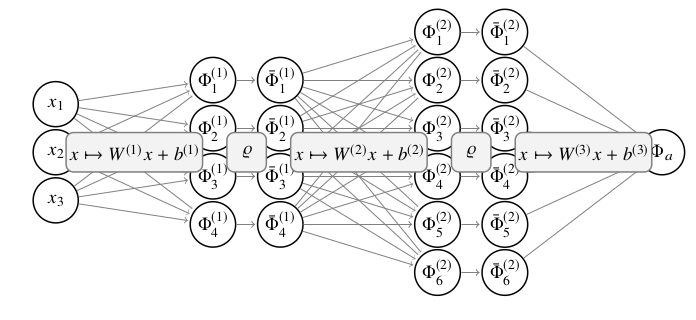
\includegraphics[width=0.5\linewidth]{img/ejemplo_red.png}
\caption{Grafo de una red completamente conectada simple de arquitectura \(a=((3,4,6,1),\mathcal{q})\) donde el primer elemento describe el número de neuronas por capa y el segundo la función de activación. Obtenida en Grohs et al.\cite{matesModernasDL}}.
\label{fig:img1}
\end{figure}


Tras dar una primera aproximación a las redes neuronales completamente conectadas, se comenta que el término redes neuronales profundas hará siempre referencia a esta definición.

Como ya se mencionó anteriormente, las redes neuronales profundas son algoritmos usados en tareas como la clasificación o la regresión que, a partir de cierto subconjunto (de entrenamiento) de un espacio medible, generaliza a datos de otros subconjuntos disjuntos al usado en el entrenamiento. Esto lleva a pensar que, como todo problema en inteligencia artifical, en función de la situación es conveniente usar o no ciertas características determinantes para resolver el problema: la profundidad, las funciones de activación, el número de neuronas por capas,$\dots$. Además, se busca que generalice bien y no sea solo capaz de hacer bien las tareas del conjunto de entrenamiento (sobreajuste), aún queriendo minimizar la función de coste. Estas ideas llevan a pensar en cierto conjunto de posibles algoritmos obtenidos a partir de la arquitectura de una red.

\begin{definicion} [Conjunto de hipótesis de redes neuronales]
Sea $a=(N,\mathcal{q})$ una arquitectura de red neuronal con dimensión de datos de entrada $N_0 = d \in \mathbb{N}$ y de salida $N_L=1$, donde $\mathcal{q}$ es la función de activación (medible). El conjunto de hipótesis de redes neuronales se define de dos maneras en función del tipo de problema:
\begin{itemize}
	\item \textbf{Problema de regresión}: $$\mathcal{F}_a = \{\phi_a(\text{·},\theta): \theta \in \mathbb{R}^{P(N)}\}$$
	\item \textbf{Problema de clasificación}: Con $sgn$ la función signo $$\mathcal{F}_{a,sgn} = \{sgn(\phi_a(\text{·},\theta)):\theta \in \mathbb{R}^{P(N)}\}$$
\end{itemize}
\end{definicion}

Se podría pensar con la definición anterior que basta con ajustar ciertas características de la red para obtener un buen algoritmo que permita generalizar no solo la forma en que los datos entran para ser clasificados, sino también el problema al que estamos enfrentando, siempre que se tenga claro si va a ser de regresión o de clasificación. Esta idea es errónea, tal y como se probará con el siguiente teorema, previas definiciones y resultados para poder construirlo adecuadamente. Gracias a este resultado se podrá entender más adelante porqué no existen algoritmos de ataque o defensa genéricos para cualquier red.

En primer lugar, volviendo a la primera definición dada en el capítulo, se escribe $s=(z^{(i)})_{i=1}^{m}$ a los $m$ datos de un subconjunto de entrenamiento del espacio medible $\mathcal{Z}$. A partir de ahora, se consideran las variables aleatorias e idénticamente distribuidas $Z^{(1)},\cdots,Z^{(m)}$ de cierto vector aleatorio $Z$, cuyas realizaciones se corresponden a los datos $z^{(1)},\cdots,z^{(m)}$ respectivamente, se podría escibir como $z$. Por otro lado, se menciona que $Z$ va a seguir una distribución dada por $I_Z$ en el espacio $\mathcal{Z}$.

\begin{definicion} [Riesgo]

Para toda función $f \in \mathcal{M(X,Y)}$ se define el riesgo como $$\mathcal{R}(f):=\mathbb{E}[\mathcal{L}(f,Z)] = \int_{\mathcal{Z}}\mathcal{L}(f,z) dI_Z(z)$$

Se define también el riesgo para cierta función condicionada a $S$ (vector de variables aleatorias independientes e idénticamente distribuidas, con $f_S=\mathcal{A}(S)$ el modelo asociado a la condicionada), como  
$$\mathcal{R}(f_S)=\mathbb{E}[\mathcal{L}(f_S,Z)|S]$$

\end{definicion}

En líneas generales, se puede observar que el riesgo es ximplemente esperanza matemática de la función asociada al algoritmo.

Para las tareas de predicción se podría escribir $Z = (X,Y)$, esto es, los datos que entran y las respectivas predicciones, por ser $X$ una variable aleatoria que toma valores en $\mathcal{X}$ e Y la respectiva en $\mathcal{Y}$. En los problemas de clasificación, la probabilidad de no predecir bien es

$$\mathcal{R}(f) = \mathbb{E} \left[ \mathbb{1}_{(-\infty,0)} (Yf(X)) \right]$$ 

Además, para datos con ruido es conveniente hacer la siguiente definición.

\begin{definicion} [Función óptima de Bayes]

Teniendo en cuenta la definición anterior, se dirá que $f^{*} \in \mathcal{M(X,Y)}$ es la función óptima de Bayes si minimiza la esperanza, esto es, su riesgo asociado es

$$\mathcal{R}^{*}:= \inf_{f \in \mathcal{M(X,Y)}} \mathcal{R}(f)$$

Nótese que sería incorrecto decir que $\mathcal{R}^{*}=\mathcal{R}(f^{*})$ pues el conjunto $\mathcal{M(X,Y)}$ no es necesariamente compacto, luego puede no alcanzar el mínimo.

\end{definicion}

Los problemas que ocupan a las redes neuronales son los de regresión y clasificación en general, por lo que se puede obtener el riesgo asociado a cada uno de ellos de manera explícita.

\begin{lema}
Considérense $X$ e $Y$ variables aleatorias. El riesgo toma las siguientes expresiones si:
\begin{itemize}
	\item \textbf{Regresión}: Supuesto que $Var[Y] < \infty$, entonces
$$\mathcal{R}(f)=\mathbb{E}[(f(X)-\mathbb{E}[Y|X])^{2}] + \mathcal{R}^{*}$$
alcanzando el mínimo en $f^{*}(x)=\mathbb{E}[Y|X=x]$ para cierto $x \in X \subset \mathcal{X}$.
	\item \textbf{Clasificación}: La expresión viene dada por 
	$$\mathcal{R}(f) = \mathbb{E}[ \left| \mathbb{E}[Y|X] \right| \mathbb{1}_{(-\infty,0)}\left(\mathbb{E}[Y|X]f(X)\right) ] + \mathcal{R}^{*}$$ que alcanza el mínimo en $f^{*}(x)=sgn(\mathbb{E}[Y|X=x])$ para cierto $x \in X \subset \mathcal{X}$.
\end{itemize}
\end{lema}

\begin{lema}\label{lemaNFL}
Sea $\{a_n\}$ una sucesión de números positivos convergente a $0$, tal que $a_1 \leq \frac{1}{16}$. Entonces, se puede encontrar una distribución de probabilidad tal que sus valores $(p_1, p_2, \ldots)$ cumplen $p_1 \geq p_2 \geq \cdots$, y dado $n \in \mathbb{N}$ es cierto que
$$\sum_{i=n+1}^{\infty} p_i \geq \max(8a_n, 32np_{n+1}).$$

\end{lema}

\begin{proof}
Basta encontrar una forma de caracterizar $p_i$ de tal manera que se cumpla

$$\sum_{i=n+1}^{\infty}p_i \geq \max(8a_n,32np_n)$$

Sean los naturales $u < v$, se define $H(v,u)=\sum_{i=u}^{v-1} \frac{1}{i}$. Puede ser encontrada una sucesión de naturales $1=n_1 < n_2 < \dots$ tales que cumplen:
\begin{itemize}
	\item $H(n_{k+1},n_k)$ es creciente.
	\item $H(n_2,n_1) \geq 32$.
	\item $8a_{n_k} \leq \frac{1}{2^k}$ para $k \geq 1$.
\end{itemize}

Para que lo anterior sea cierto, sobre todo la tercera afirmación, se necesita la hipótesis de $a_1 \leq \frac{1}{16}$. Ahora, se define la sucesión $\{c_k\}_{k \in \mathbb{N}}$ como 
$$c_k = \frac{32}{2^kH(n_{k+1},n_k)} \text{ para todo } k \geq 1$$
que es decreciente y resolviendo una serie geométrica se cumple la igualdad 
$$\frac{1}{32}\sum_{k=1}^{\infty} c_kH(n_{k+1},n_k)=\sum_{k=1}^{\infty} \frac{1}{2^k}=1$$

Sea ahora $n \in [n_k,n_{k+1})$, y para dicho natural $p_n = \frac{c_k}{32n}$ con $k \in \mathbb{N}$. Se puede observar que $\{p_n\}$ decrece y

$$\sum_{n=1}^\infty p_n = \sum_{k=1}^{\infty} \frac{c_k}{32} H(n_{k+1},n_k) = 1$$

Finalmente, para todo $n \in [n_k,n_{k+1}),$

\[
\sum_{i=n+1}^{\infty} p_i \geq \sum_{j=k+1}^{\infty} \frac{c_j}{32}H(n_{j+1},n_j) = \sum_{j=k+1}^{\infty} \frac{1}{2^j} = \frac{1}{2^k}
\]

Por la monotonía de $H(n_{k+1},n_k)$, es cierto que $\frac{1}{2^k} \geq c_k = 32np_n$. Por otro lado, $\frac{1}{2^k} \geq 8a_{n_k} \geq 8a_n$, por lo que queda probado el lema.

\end{proof}

Finalmente, se prueba que no existe un algoritmo universal para los problemas que enfrentan las redes neuronales profundas suponiendo distribuciones cualesquiera.

\begin{teorema}[No Free Lunch]

Sea $\{a_n\}_{n \in \mathbb{N}}$ una sucesión de números reales positivos convergente a cero, tal que $a_1 \leq \frac{1}{16}$. Para cualquier algoritmo de aprendizaje para una tarea de clasificación específica $\mathcal{A}$, existe una distribución $I_Z$ desprendida de la distribución $(X,Y)$ tal que, dado $n \in \mathbb{N}$ y cierto conjunto de entrenamiento $S \sim I_Z^n$, se cumple lo siguiente:

$$\mathbb{E}[\mathcal{R}(\mathcal{A}(S))] \geq \mathcal{R}^{*}+a_n$$

\end{teorema}

Antes de comenzar la prueba tal y como se ve en Devroye et al.~\cite{demoNFL} se especifica que un algoritmo de aprendizaje $\mathcal{A}$ es en realidad una secuencia de instrucciones $\{f_n\}$ tal que el error asociado a cada una de ellas para el problema de clasificación, converge a $\mathcal{R}(f^*)$. Por ello, es necesario introducir la siguiente definición.

\begin{definicion}
Las reglas de clasificación serán consistentes para cierta distribución si la sucesión de riesgos esperados converge al menor error, esto es
$$\lim_{n \to \infty} \mathcal{R}(f_n) = \mathcal{R}(f^*)=\mathcal{R}^*$$.
Además, serán fuertemente consistentes si 

$$\mathbb{P}[\lim_{n \to \infty} \mathcal{R}_n = \mathcal{R}^*] = 1$$
\end{definicion}

Este teorema se puede reescribir de la siguiente manera, que será probada.

Sea $\{a_n\}$ una sucesión de positivos convergente a $0$ tal que $a_1 \leq \frac{1}{16}$. Para cada regla, existe una distribución existe una distribución con riesgo nulo tal que 

$$\mathbb{E}[L_n] \geq a_n$$

para todo $n \in \mathbb{N}$ y $L_n$ el error de la probabilidad condicionada según el algoritmo.

\begin{proof}

Consideremos $b=0.b_1b_2b_3\ldots \in [0,1]$ y $B$ una variable aleatoria uniformemente distribuida en $[0,1]$ que escribimos como $B=0.B_1B_2B_3\ldots$. Consideremos ahora la variable aleatoria $X$ tal que cumpla 
$$\mathbb{P}[X=i]=p_i$$
donde $p_i \geq p_{i+1} > 0$ $i\geq 1$ y $\sum_{i=n+1}^{\infty} p_i \geq \max(8a_n,32np_{n+1})$ para $n \in \mathbb{N}$. Nótese que $\{p_n\}_{n \in \mathbb{N}}$ es una sucesión que verifica el lema \ref{lemaNFL}. Sea ahora $Y=b_X$, función dependiente de $X$,  que tiene riesgo asociado $0$. En función de $b \in [0,1)$ va a describir distribuciones distintas, obteniendo una distribución aleatoria si se sustituye por $B$. Escribimos $\Delta_n = ((X_1,B_{X_1}),\ldots,(X_n,B_{X_n}))$ y se define $G_{ni} = f_n(i,\Delta_n)$. Si $L_n(B)$ es la probabilidad de error en un distribución aleatoria, se puede expresar como
$$L_n(B)=\sum_{i=1}^{\infty} p_iI_{\{G_{ni} \neq B_i\}}$$

y si $L_n(b)$ es la probabilidad del error en una distribución parametrizada por $b$, entonces se cumple que

$$\sup_{b} \inf_{n} \mathbb{E} \left[ \frac{L_b(b)}{2a_n} \right] \geq \sup_{b}\mathbb{E}\left[\inf_{n}\frac{L_n(b)}{2a_n}\right] \geq \mathbb{E}\left[\inf_{n}\frac{L_n(B)}{2a_n}\right] = \mathbb{E}\left[\mathbb{E}\left[\inf_{n}\frac{L_n(B)}{2a_n} \bigg| X_1,X_2,\ldots\right]\right]$$

Por otro lado, es cierto que

\begin{align*}
\mathbb{E}\left[ \inf_{n}\frac{L_n(B)}{2a_n} \bigg| X_1,X_2,\ldots \right] &\geq \mathbb{P} \left[ \bigcap_{n=1}^{\infty} \{L_n(B) \geq 2a_n\} \bigg| X_1,X_2,\ldots \right] \\
&\geq 1 - \sum_{n=1}^{\infty} \mathbb{P}\left[ L_n(B) < 2a_n \bigg| X_1,X_2,\cdots \right] \\
&= 1 - \sum_{n=1}^{\infty} \mathbb{P}\left[ L_n(B) < 2a_n \bigg| X_1,_2,\ldots, X_n \right] \\
&= 1 - \sum_{n=1}^{\infty} \mathbb{E} \left[ \mathbb{P} \left[ L_n(B) < 2a_n \bigg| \Delta_n \right] \bigg| X_1,X_2,\ldots,X_n \right]
\end{align*}

A continuación, se usa el concepto de dominancia estocástica por la hipótesis de que $\{p_n\}_{n \in \mathbb{N}}$ es decreciente

\begin{align*}
\mathbb{P}\left[ L_n(B) < 2a_n \,|\, \Delta_n \right] &\leq \mathbb{P} \left[ \sum_{i \notin \{X_1,\ldots,X_n\}} p_i I_{(G_{ni} \neq B_i)} < 2a_n \bigg| \Delta_n \right] \\
&= \mathbb{P}\left[ \sum_{i \notin \{X_1,\ldots,X_n\}} p_iI_{\{B_i=1\}} < 2a_n \bigg| \Delta_n \right] \leq \mathbb{P}\left[ \sum_{i=n+1}^{\infty}  p_iI_{\{B_i=1\}} < 2a_n \right] \\ &= \mathbb{P}\left[ \sum_{i=n+1}^{\infty} p_iB_i < 2a_n \right]
\end{align*}

Para concluir la demostración, se tendrá que usar el método de acotación de Chernoff (véase resultados previos), apoyado en la desigualdad de Markov:

\begin{align*}
\mathbb{P}\left[ \sum_{i=n+1}^{\infty} p_iB_i < 2a_n \right] &\leq \mathbb{E}\left[ e^{2sa_n - s\sum_{i=n+1}^{\infty} p_iB_i} \right] \\ 
&= e^{2sa_n}\prod_{i=n+1}^{\infty}\left(\frac{1}{2} + \frac{1}{2}e^{-sp_i}\right) \leq e^{2sa_n}\prod_{i=n+1}^{\infty}\frac{1}{2}\left(2-sp_i+\frac{s^2p_i^2}{2}\right) \\
&\leq \exp\left(2sa_n + \sum_{i=n+1}^{\infty}\left(-\frac{sp_i}{2}+\frac{s^2p_i^2}{4}\right)\right) \text{ (y como } 1-x \leq e^{-x} \text{)} \\
& \leq \exp\left( 2sa_n - \frac{s\Sigma}{2} + \frac{s^2p_{n+1}\Sigma}{4}\right) \text{ (donde } \Sigma = \sum_{i=n+1}^{\infty} p_i  \text{)} \\
&= \exp\left(-\frac{1}{4} \frac{(4a_n - \Sigma)^2}{p_{n+1}\Sigma} \right)
\end{align*}

teniendo en cuenta que $\Sigma > 4a_n $ y tomando $s = \frac{\Sigma - 4a_n}{p_{n+1}\Sigma}$ se sigue que 

\begin{align*}
\exp\left(-\frac{1}{4} \frac{(4a_n - \Sigma)^2}{p_{n+1}\Sigma} \right) \leq \text{exp}\left( -\frac{1}{16} \frac{\Sigma}{p_{n+1}} \right)
\end{align*}
pues además $\Sigma \geq 8a_n$. Como es cierto $\Sigma \geq 32np_{n+1}$ se concluye que

\begin{align*}
\text{exp}\left( -\frac{1}{16} \frac{\Sigma}{p_{n+1}} \right) \leq e^{-2n}
\end{align*}

por lo que

\begin{align*}
\sup_{b}\inf_{n} \mathbb{E} \left[ \frac{L_n(b)}{2a_n} \right] \geq 1 - \sum_{n=1}^{\infty} e^{-2n} = \frac{e^2-2}{e^2-1} > \frac{1}{2}
\end{align*}

Así, existe un $b$ que cumple lo que se quería probar para todo $n \in \mathbb{N}$

\end{proof}

%Para ilustrar un ejemplo en el que el teorema anterior puede ser usado para ver que no existe un algoritmo universal para todos los problemas de clasificación es el siguiente: seleccionado $\mathcal{F}$ el conjunto de hipótesis, sea $f_{\mathcal{F}}^* \in \text{argmin}_{f \in \mathcal{F}} \mathcal{R}(f)$ la mejor aproximación tal que

%\begin{align*}
%\mathcal{R}(f_S)-R^* &= \mathcal{R}(f_S)- \hat{\mathcal{R}}_S(f_S)+\hat{\mathcal{R}}_S(f_S)-\hat{\mathcal{R}}_S(f_\mathcal{F}^*) + \hat{\mathcal{R}}_S(f_\mathcal{F}^*) - \mathcal{R}_S(f_\mathcal{F}^*) + \mathcal{R}_S(f_\mathcal{F}^*) - \mathcal{R}^*
%\end{align*}


%\begin{align*}
% \leq \epsilon^{\text{opt}} + 2\epsilon^{\text{gen}}+\epsilon^{\text{approx}}
%\end{align*}

Es conveniente remarcar la forma en que una red neuronal profunda puede aprender. Tal y como se observa en \ref{fig:img1}, cada capa con neuronas tienen una serie de funciones de activación. La manera de entrenar y transmitir la información entre las neuronas es a través de la técnica backpropagation. Con esta manera el error en la red se propaga tanto adelante como atrás, siendo la forma más común de hacerlo el cálculo de los gradientes, por lo que es fundamental el uso de la regla de la cadena. La regla de la cadena facilita el control de cómo pequeños cambios en los pesos y sesgos de una capa afectan a la función de pérdida final, lo que es esencial para el ajuste adecuado de los parámetros de la red neuronal.

El clásico algoritmo para permitir que la red aprenda es el gradiente estocástico descendente, que se apoya en hiperparámetros tales como la tasa de aprendizaje. La expresión fundamental de este algoritmo es 

$$\Theta^{(k)} = \Theta^{(k-1)} - \frac{\eta_k}{m'}\sum_{z \in S'} \triangledown_\theta\mathcal{L}(\phi_a(\cdot,\Theta^{(k-1)}),z) $$

siendo $\Theta_k$ los pesos en la red en la iteración $k$ y $m' \leq m$ el tamaño de batch escogido $S'$ de un dataset de entrenamiento $S$.

Una pregunta que podría hacerse es cuán rápido aprende la red para un algoritmo basado en gradiente estocástico descendente. El siguiente teorema no solo asegura la convergencia del algoritmo, sino que trata sobre la velocidad de convergencia del mismo.

\begin{teorema}
Se escribe $D^{(k)}=\triangledown r(\Theta^{(k-1)})$ y $r(\theta)=\hat{\mathcal{R}}_s(\phi_a(\cdot,\theta))$. Sean $p,K \in \mathbb{N}$ y $r:B(0,1) \to \mathbb{R}$ con $B(0,1) \subset \mathbb{R}^p$, siendo $r$ diferenciable y convexa. Sea $(\Theta^{(k)})_{k=1}^{K}$ el conjunto de pesos de cada capa con inicialización $\Theta^{(0)}=0$, tasa de aprendizaje $\eta_k=K^{-\frac{1}{2}}$ para $k=\{1,...,K\}$ y las variables aleatorias $(D^{(k)})_{k=1}^{K}$ que se encuentran casi seguro en la bola unidad, esto es, $||D^{(k)}||_2 \leq 1$. Entonces


$$\mathbb{E}[r(\overline{\Theta})] - r(\theta^*) \leq \frac{1}{\sqrt{K}}$$

donde $\overline{\Theta} := \frac{1}{K} \sum_{k=1}^{K} \Theta^{(k)}$ y $\theta^* \in argmin_{\theta \in B(0,1)} r(\theta)$.
\end{teorema}

Generalmente las redes neuronales con 2 capas son aproximadores universales, es decir, suponiendo una función de activación $\mathcal{q}$ la red neuronal puede aproximar cualquier función continua, por muy compleja que sea, sobre un conjunto compacto. Para acabar el apartado, se enuncia y demuestra el siguiente teorema, siendo necesarios algunos resultados del análisis funcional.

\begin{teorema}[Teorema de aproximación universal]
Sean $d \in \mathbb{N}$, $K \subset \mathbb{R}^d$ un compacto, y $\mathcal{q} \in L_{loc}^{\infty}(\mathbb{R})$ una función de activación tal que la adherencia del conjunto de puntos de discontinuidad de la misma es un conjunto de Lebesgue nulo. Considérese

$$\tilde{\mathcal{F}} = \bigcup_{n \in \mathbb{N}} \mathcal{F}_{((d,n,1),\mathcal{q})}$$


el conjunto de realizaciones de una red neuronal de dos capas. Entonces existe cierto subespacio $C(K) \subset cl(\tilde{\mathcal{F}})$ de funciones continuas sobre $K$ si y solo si no existe ningún polinomio $p: \mathbb{R} \to \mathbb{R}$ tal que $p=\mathcal{q}$ casi por doquier ($cl(\tilde{\mathcal{F}}$ es la adherencia de $\tilde{\mathcal{F}}$ se toma con respecto a la topología inducida por la norma $L^{\infty}(K)$).
\end{teorema}

\begin{proof}
Apoyándose en el teorema de Hahn-Banach, se obtiene que el que $\tilde{\mathcal{F}}$ sea denso sobre cierto espacio vectorial real normado $\mathcal{S}$ es equivalente a afirmar que para todos aquellos funcionales no triviales $F \in \mathcal{S}'-\{ 0 \}$ que estén en el espacio dual topológico de $\mathcal{S}$ existen ciertos parámetros $w \in \mathbb{R}^d$, $b \in \mathbb{R}$ tales que cumplen

$$F(\mathcal{q}(\langle w,\cdot \rangle + b)) \neq 0$$

En el caso en que $\mathcal{S} = C(K)$ entonces por el teorema de representación de Riesz-Markov-Kakutani se tiene que $\mathcal{S'}$ es un espacio de medidas de Borel sobre $K$. Por lo tanto el teorema se prueba si $\mathcal{q}$ es discriminatoria, esto es, $\mathcal{q}$ es tal que para una medida de Borel $\mu$, cumple

$$\int_{K} \mathcal{q}(\langle w,x \rangle + b)d\mu(x) = 0$$

para $w \in \mathbb{R}^d$ y $b \in \mathbb{R}$ si $\mu = 0$. Por ejemplo, si fuese una función activadora sigmoide, sería discriminatoria.

Supóngase que $\mathcal{q}$ es discriminatoria para todo $w \in \mathbb{R}^d$, $b \in \mathbb{R}$. Como para $x \in \mathbb{R}^d$ se tiene que $\mathcal{q}(ax+b) \to \mathbb{1}_{(0,\infty)}(x) + \mathcal{q}(b)\mathbb{1}_{\{0\}}(x)$ si $a \to \infty$, por hipótesis y pasando al límite para $c_1,c_2,b \in \mathbb{R}$, $w \in \mathbb{R}^d$, se obtiene

\[
\int_{K} \mathbb{1}_{[c_1,c_2]}(\langle w,x \rangle + b) \, d\mu(x) = 0
\]

Para finalizar, si se representa la exponencial $e^{-2\pi i x}$ como límite de suma de funciones elementales, lleva a deducir que

\[
\int_{K} e^{-2\pi i (\langle w,x\rangle + b)} \, d\mu(x) = 0.
\]

Por lo tanto, al anularse la transformada de Fourier de $\mu$, se concluye que $\mu = 0$.

\end{proof}

Hasta ahora se ha probado para funciones compactas sobre un espacio compacto. Sin embargo, se puede extender a funciones medibles usando el teorema probado como apoyo, el teorema de Lusin y la medida de Lebesgue.

\section{Aprendizaje adversario}

Los algoritmos de aprendizaje profundo, al igual que el resto de tecnologías informáticas, son propensos a recibir ataques para hacerles fallar. Por ello, el interés por el desarrollo de algoritmos más robustos frente a dichos ataques crece cada vez más, sobre todo con el gran impacto que la inteligencia artificial está teniendo en la vida cotidiana de las personas.

\subsection{Ataques adversarios}

Es adecuado tratar este tipo de ataques como un caso aparte a los clásicos ataques a sistemas informáticos (virus, troyanos,...) ya que la forma de actuar o los objetivos pueden ser distintos. Se denominan ataques adversarios.

Los ataques adversarios pueden ser clasificados según la forma en que actua, conocimientos del algoritmo,... Por ejemplo, se podría clasificar de la siguiente manera (seguida en Joseph et al.~\cite{LibroAdvMachL}):
\begin{itemize}
	\item \textbf{Ataques causativos}: Aprovechan las debilidades que presentan los datos de entrenamiento (mala calidad, escasez,...).
	\item \textbf{Ataques exploratorios}: Orientados a llevar al fallo a modelos ya entrenados que estén en fase de test o ya en uso por otros usuarios.
\end{itemize}

Otras formas de clasificar estos ataques puede ser la propuesta en Zhou et al.~\cite{ArtCentralInfo}:
\begin{itemize}
	\item \textbf{Objetivo del atacante}:
	\begin{itemize}
		\item \textbf{Ataques de envenenamiento}: Los atacantes acceden y modifican el dataset de entrenamiento, haciendo que el sistema no dé los resultados esperados.
		\item \textbf{Ataques de evasión}: Dada una red profunda entrenada, sin poder alterar los pesos, el atacante accede y modifica el dataset de test para conducir al algoritmo a fallar.
	\end{itemize}
	\item \textbf{Conocimiento del sistema atacado}: 
	\begin{itemize}
		\item \textbf{Ataques de caja blanca}: El atacante conoce toda o parte de la información que describe al modelo, creando ataques en base a ella.
		\item \textbf{Ataques de caja negra}: El atacante desconoce las características del algoritmo, por lo que los ataques se dirigen a obtener información del sistema.
	\end{itemize}
	\item \textbf{Comportamiento del algoritmo}:
	\begin{itemize}
		\item \textbf{Ataques sin etiqueta}: El propósito del ataque es hacer que el algoritmo falle una predicción, sin importar el resultado.
		\item \textbf{Ataques con etiqueta}: El ataque hará que el algoritmo falle en su predicción, acorde a lo que especifique el atacante.
	\end{itemize}
\end{itemize}

Nótese que la clasificación no es excluyente entre si. Es decir, un ataque puede ser clasificado tanto de envenenamiento como de ataque con etiqueta.

En la Figura \ref{fig:ataques_scheme} se muestra un esquema general en lo que respecta al ataque según objetivo del atacante.

\begin{figure}[!htbp]
    \centering
    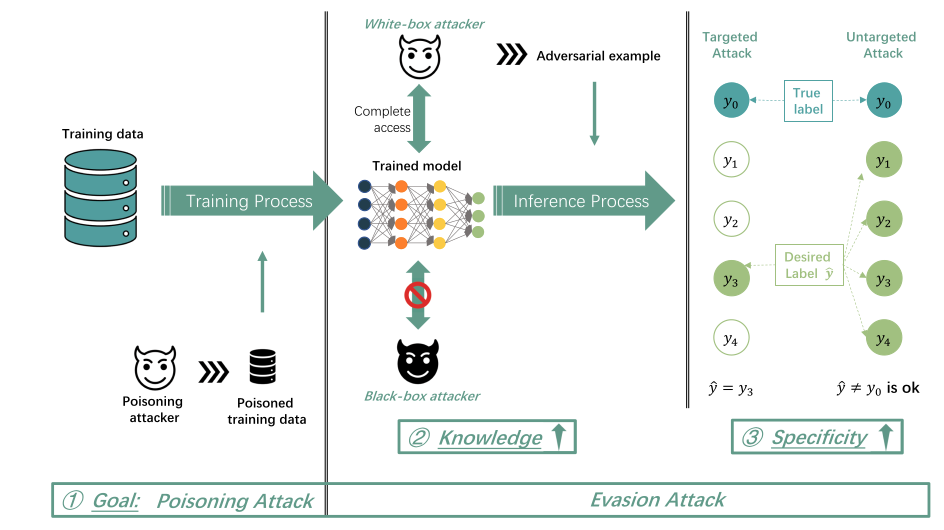
\includegraphics[width=1.0\textwidth]{ataque_objetivo_atacante.png}
    \caption{Imagen que ilustra el esquema general de la forma de atacar a una red neuronal profunda. Obtenida en Rodrigo et al.~\cite{RodrigoTFM}}
    \label{fig:ataques_scheme}
\end{figure}

Si bien es más fácil ver la acción de estos ataques en redes convolucionales para clasificación de imágenes, es posible  adaptar un ataque a cualquier tipo de red, como las redes recurrentes, los modelos LLM, etc. Un ejemplo de ataque a una red convolucional, en que se añade ruido imperceptible al ojo humano, es el que aparece en la Figura \ref{fig:example_fgsm}.

\begin{figure}[h]
    \centering
    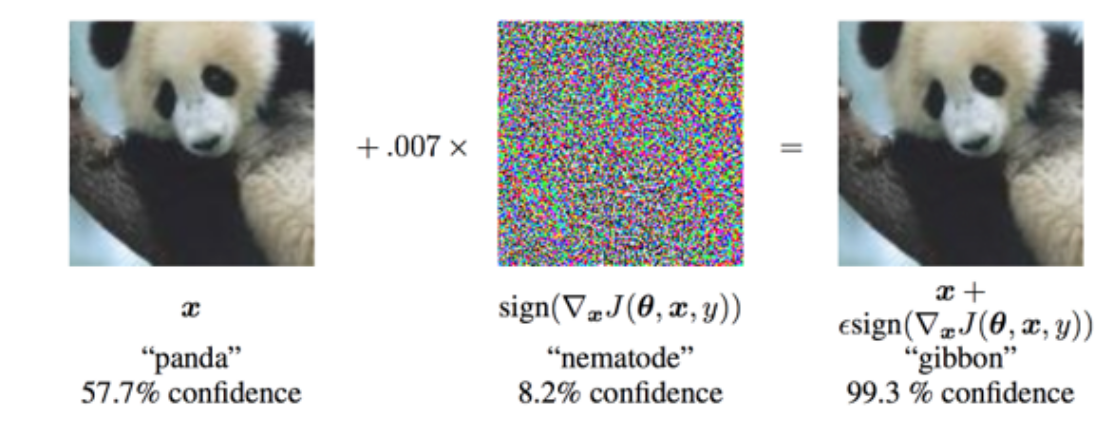
\includegraphics[width=0.7\textwidth]{example_fgsm.png}
    \caption{Ejemplo de ataque FGSM a una red entrenada en Goodfellow et al.~\cite{GoodfLAdvers}}
    \label{fig:example_fgsm}
\end{figure}


La existencia de tales ataques hace pensar en cómo podrían ser evitados, y para ello hay que pensar en qué está fallando en la red para poder ser atacada. Muchos investigadores discuten entre las vulnerabilidades que presentan las redes neuronales, sin llegar a un acuerdo que establezca un paradigma universal de defensa de estos algoritmos.

Por un lado, Ilyas et al.~\cite{NoRobustFeatures} consigue probar que una de las causas es el aprendizaje de características no robustas. Gilmer et al.~\cite{RelatDimensAdvEx} culpa a la alta dimensionalidad de los datos, mientras que otros como Schmidt et al.~\cite{RequiresDataLudwig} estima que se debe a la poca presencia de datos.

También hay otros estudios que buscan las vulnerabilidades al modelo. Por ejemplo, mientras en Szegedy et al.~\cite{DataManifold} culpa a la no linealidad de modelos, otros como Goodfellow et al.~\cite{GoodfLAdvers} y Fawzi et al.~\cite{FundLimits} culpan a la linealidad de los algoritmos, siendo visiones claramente enfrentadas. Además, otros estudios sugieren otras vulnerabilidades como los límites de decisión de la red, o la forma de entrenar a la red.

\subsection{Técnicas de defensa}

Presentada una clasificación de los posibles ataques, y las vulnerabilidades expuestas tanto en los datos como en el propio modelo, es natural intentar idear maneras de entrenar a un algoritmo de aprendizaje profundo para minimizar, o incluso evitar, el daño ocasionado por estos ataques. A continuación se listan algunas técnicas usadas para la mitigación del daño:
\begin{itemize}
	\item \textbf{Robustez de la red}: Mediante el uso de técnicas como la introducción de capas dropout, se podría conseguir que el algoritmo aprendiese características robustas, esto es, identifican al objeto a detectar, pero de una manera más óptima, frente a otras posibles características.
	\item \textbf{Aumento de datos}: La red podría aprender las características que identifican mejor a un objeto de la imagen si el mismo se encuentra en distintas situaciones. Haría que la red generalizase mejor.
	\item \textbf{Detección de datos envenenados}: Aunque muchos datos envenenados serían imposibles de distinguir para un humano, se han desarrollado algoritmos que, dado un dataset, puedan detectar qué datos han sido alterados bajo cierta precisión.
\end{itemize}

\endinput
%--------------------------------------------------------------------
% FIN DEL CAPÍTULO. 
%--------------------------------------------------------------------
% !TeX root = ../tfg.tex
% !TeX encoding = utf8

\chapter{Análisis de vulnerabilidades de redes neuronales profundas}
\label{cap:capitulo2}

Los ataques causativos son aquellos que aprovechan ciertas propiedades vulnerables de los datos para que el modelo entrenado tenga el comportamiento buscado por el atacante. Un ejemplo de caso en el que se muestra que los datos y lo que representan son una parte crucial en el aprendizaje automático es el siguiente: el ejercito de cierto país desarrolla un algoritmo de aprendizaje profundo para la detección en tiempo real de tanques y, tras gastar grandes cantidades de dinero, obtienen un modelo que proceden a testear. Los resultados arrojan que el modelo es incapaz de reconocer tanques en diversos escenarios, o incluso reconoce tanques cuando no aparecen en la imagen. Finalmente, se descubrió que el modelo fue entrenado con imágenes de tanques en cierto momento del día, y el modelo aprendió a reconocer tanques únicamente por el color del cielo.

Aunque el caso anterior está relacionado con la calidad de los datos, se podría extrapolar a ataques causativos. Un posible atacante podría ser un hipotético país rival, que tiene la intención de atacar al país que desarrolló el modelo. Si ataca a los datos de entrenamiento para que el modelo no aprenda buenas características, podría atacar en un momento en que sabe que el modelo fallará en la detección de sus tanques.

Esta situación ocurrió en los años 80 cuando el ejercito estadounidense intentó crear un modelo que reconociese tanques.%, y los clasificase como aliados o enemigos.

Se puede observar que actualmente ningún modelo de redes neuronales profundas está exento de este tipo de ataques, al menos tal y como se entrenan actualmente. Es natural preguntarse por el origen de estos ataques: qué está fallando en la parte de los datos. Por ello, varios investigadores de distintos campos empezaron a buscar justificaciones de la existencia de los mismos, intentando demostrar las vulnerabilidades existentes en estos modelos, tanto desde el punto de vista de los datos (ataques causativos) como desde el punto de vista del entrenamiento del modelo (ataques exploratorios), presentando bastantes argumentos a favor de algunas debilidades, expandiendo el objeto de estudio a campos como la topología algebraica o la geometría de la información.

A continuación, se exponen algunos de los resultados más importantes obtenidos hasta la fecha, acompañados de justificaciones teóricas sobre las que se apoyan. Se remarca que estos resultados distinguen entre la vulnerabilidad de los datos, haciendo hincapié en las distribuciones que puedan seguir, y la vulnerabilidad del modelo, ya sea por existencia de ciertas capas o por otros motivos, tales como la función de activación de neuronas.

% VULNERABILIDADES DE LOS DATOS

\section{Dimensionalidad de los datos}
\subsection{Límites del riesgo adversario}
En este apartado se presentarán los resultados justificados en  Diochnos et al.~\cite{LimitsAdvers}, con los que se muestra que no se pueden superar ciertos niveles de seguridad en un modelo teniendo como hipótesis que los datos se distribuyen en el espacio de características binarias de gran dimensionalidad (\(\{0,1\}^n\)) de manera uniforme, usando los autores una serie de resultados de apoyo.



\begin{definicion}{}[Tamaño local de la bola de Hamming]
Para $n \in \mathbb{N}$, se define localmente el tamaño de la bola de Hamming como la función $\text{BSize}_n: \{1,\ldots,n\} \times [0,1) \to [0,1)$ definida de la siguiente forma: 

$$\text{BSize}_n(k,\lambda)=2^{-n}\cdot \left( \sum_{i=0}^{k-1} \binom{n}{i} + \lambda\cdot\binom{n}{k} \right)$$

\end{definicion}

\begin{lema} \label{lem21}
Para $\mu \in [0,1]$ se cumple

\[
\mu \geq \text{BSize}_n\left(\frac{n-\sqrt{-2\cdot\ln(\mu)\cdot n}}{2}+1,0\right)
\]

Además, si $\text{BSize}_n^{-1}(\mu)$ es la inversa (por ser $\text{BSize}_n$ biyectiva $\forall n \in \mathbb{N}$), entonces 
$$k \geq \frac{n-\sqrt{-2\cdot ln(\mu)\cdot n}}{2}+1$$
\end{lema}

Para la prueba, se usará el siguiente resultado.

\begin{lema}[Caso general de la desigualdad de Hoeffding] \label{Hoefding}
Sean $X_1,...,X_n$ variables aleatorias independientes. Supóngase que $X_i$ está acotada de tal manera que 

$$\mathbb{P}[X_i \in [a_i,b_i]] = 1$$

La media muestral se define como $\bar{X} = \frac{1}{n} \sum_{i=1}^n X_i$

Entonces

\begin{equation}
\mathbb{P}[\bar{X} - \mathbb{E}[\bar{X}] \geq t] \leq \exp \left( - \frac{2t^2n^2}{\sum_{i=1}^n (b_i-a_i)^2} \right)
\end{equation}

\begin{equation}
\mathbb{P}[|\bar{X}-\mathbb{E}[\bar{X}]| \geq t] \leq 2 \cdot \exp \left( - \frac{2t^2n^2}{\sum_{i=1}^n (b_i - a_i)^2} \right)
\end{equation}

para todo $t > 0$.

\end{lema}

\begin{proof}(Lema \ref{lem21})
Sea $k' = \frac{n-\sqrt{-2 \cdot ln(\mu)\cdot n}}{2}+1$ y sean $n$ variables aleatorias uniformes, $X_1,\ldots,X_n$ sobre el conjunto $\{0,1\}$. Se tiene $\text{BSize}_n(k',0)=\mathbb{P}[X_1+\ldots+X_n \leq K'-1]$.

Por la desigualdad de Hoefding en \ref{Hoefding}, se cumple

$$\mathbb{P}[X_1+\ldots+X_n\leq k-1] \leq e^{\frac{-n\cdot(1-\frac{2k-2}{n})^2}{2}}=\mu$$

En consecuencia, $\mu \geq \text{BSize}_n(k',0)$, por lo que se prueba la primera desigualdad. La segunda es inmediata, pues $\mu=\text{BSize}_n(k,\lambda)\geq\text{BSize}(k',0)$, lo que implica $k\geq k'$
\end{proof}

El siguiente lema se sigue del teorema central del límite.

\begin{lema} \label{lemTCL}
 Dados $\lambda \in [0,1)$ y $a \in \mathbb{R}$, si $\phi$ es la función de distribución de una normal estándar,
 
 $$\lim_{n \to \infty} \left|\text{BSize}_n\left(\frac{n}{2}+a\cdot\sqrt{n},\lambda\right)\right| = \phi(2a)
$$
\end{lema}

\begin{lema} \label{lem24}
Si $1\leq k \leq \text{E}(\frac{n}{2})$ entonces $\text{BSize}_n(k,0) < \binom{n}{k}\cdot \frac{2^{2m-1-n}}{\binom{2m}{m}}$ con $m=\text{E}(\frac{n}{2})$ (a partir de ahora, $\text{E}(x)$ será la parte entera de $x$).
\end{lema}

\begin{corolario} \label{coro21}
Si $1 \leq k \leq \text{E}\left(\frac{n}{2}\right)$ entonces $\text{BSize}_n(k, 0) < \binom{n}{k} \sqrt{\frac{n}{2^{2n+1}}}$.

\end{corolario}

\begin{proof}
Por el lema \ref{lem24}, y que se cumple $\binom{2m}{m} \geq \frac{2^{2m-1}}{\sqrt{m}}$ (véase el lema A.2 en Diochnos et al.~\cite{LimitsAdvers}), se obtiene la desigualdad
\end{proof}

\begin{corolario} \label{coro22}
Para cualquier $k \in \mathbb{N}$ se cumple $lim_{n \to \infty} \frac{\text{BSize}_n(k,0)}{\sqrt(n)\binom{n}{k}2^{-n}} \leq \sqrt{\frac{\pi}{8}}$
\end{corolario}
\begin{proof}
Sea $m=\text{E}(n/2)$. Por el lema \ref{lem24}, 

$$\frac{\text{BSize}_n(k,0)}{\sqrt{n}\binom{n}{k}2^{-n}} \leq \frac{2^{2m-1}}{\sqrt{2m}\binom{2m}{m}}$$

lo que implica $lim_{n \to \infty} \frac{\text{BSize}_n(k,0)}{\sqrt{n}\binom{n}{k}} \leq lim_{m \to \infty} \frac{2^{2m-1}}{\sqrt{2m}\binom{2m}{m}}=\sqrt{\frac{\pi}{8}}$, siendo la última desigualdad la dada en lema A.3 en Diochnos et al.~\cite{LimitsAdvers}
\end{proof}

Primero se introducirán conceptos necesarios en los teoremas, que darán lugar a una serie de corolarios que prueban lo buscado en el caso de problemas de clasificación.

\begin{definicion} \label{def22}
Dada una hipótesis de cierto espacio de hipótesis, $h$, un elemento de cierto conjunto de distribuciones sobre $\mathcal{X}$, llamando a dicho conjunto $\mathcal{D}$, se define el error asociado a la hipótesis como 
$$\text{Risk}(h,c,\mathcal{D})=\mathbb{P}[h(x)\neq c(x)]$$ para cierto $x$ escogido del conjunto de distribuciones y $c \in \mathcal{C}$ una clase (en un problema de clasificación).

\end{definicion}
\begin{definicion} \label{def23}
Para $r>0$,  $h \in \mathcal{H}$ hipótesis de cierto espacio de hipótesis, $c \in \mathcal{C}$ una clase, se define el riesgo de la región de error bajo la r-perturbación, hecha una elección $x$ en el espacio de distribuciones, como
$$\text{Risk}_r^{ER}(h,c)=\mathbb{P}[\exists x' \in B(x,r) : h(x') \neq c(x')]$$
\end{definicion}
\begin{definicion}
Para $h \in \mathcal{H}$,$x \in \mathcal{X}$,$c \in \mathcal{C}$, la robustez de la región de error asociada es, para cierta elección $x$,

$$\text{Rob}^{ER}(h,c)=\mathbb{E}[\inf\{r:\exists x' B(x,r), h(x')\neq c(x')\}]$$
\end{definicion}

En las dos definiciones anteriores $x'$ es el ejemplo adversario modificado para hacer fallar al modelo, esto es, ocurra $h(x')\neq c(x')$.

\begin{teorema} \label{tem21}
Sea \(\mathcal{P}=(\{0,1\}^n,\mathcal{Y},\mathcal{U}_n,\mathcal{C},\mathcal{H},HD)\) un problema de clasificación. Para \(h\), \(c\) y \(r \in \mathbb{N}\) sea \(\mu = \text{Risk}(h,c) > 0\) el riesgo original y \((k,\lambda)=\text{BSize}^{-1}(\mu)\) función del riesgo original. La región de error del riesgo adversario bajo una r-perturbación está acotada inferiormente como
\[
\text{Risk}_r^{ER}(h,c) \geq \text{BSize}(k+r,\lambda)
\]
\end{teorema}


La demostración del teorema implica introducir más conceptos, y es algo tediosa, por lo que no se probará. Sin embargo, las consecuencias del mismo sí se demostrarán, probando una de las debilidades de las redes neuronales profundas  que hace posible la existencia de ataques causativos.

\begin{corolario}
Sea \(\mathcal{P}=(\{0,1\}^n,\mathcal{Y},\mathcal{U}_n,\mathcal{C},\mathcal{H},HD)\) un problema de clasificación. Para cualesquiera \(h,c\) con riesgo \(\mu \in (0,\frac{1}{2}]\) asociado en la predicción de \(c\), se aumenta el riesgo de \((h,c)\) de \(\mu \in (0,\frac{1}{2}]\) a \(\mu' \in [\frac{1}{2},1]\) cambiando \(r=\sqrt{\frac{-n \ln(\mu)}{2}}+\sqrt{\frac{-n \ln(1-\mu')}{2}}\) bits en las instancias de entrada. Se tiene además que \(\text{Risk}_r^{ER}(h,c)\geq \mu'\) y si se quiere un error de \(\frac{1}{2}\), basta cambiar, como mucho, \(r'=\sqrt{\frac{-n \ln(\mu)}{2}}\) bits.
\end{corolario}
\begin{proof}
Sea \((k,\lambda)=\text{BSize}^{-1}(\mu)\). Por el teorema \ref{tem21}, se sabe que 
\[
\text{Risk}_r^{ER}(h,c) \geq \text{BSize}(k+r,\lambda)
\]
Gracias al lema \ref{lem21} se sabe \(k \geq \frac{n-\sqrt{-2 \ln(\mu)n}}{2}\). Por lo tanto
\begin{align}
\text{Risk}_r^{ER}(h,c) \geq \text{BSize}(k+r,\lambda) \\
&\geq \text{BSize}\left(\frac{n+\sqrt{-2 \ln(1-\mu')n}}{2},\lambda\right) \\
&\geq 1-\text{BSize}\left(\frac{n-\sqrt{-2 \ln(1-\mu')n}}{2}+1,0\right) \geq \mu'
\end{align}

Si el error fuese \(\frac{1}{2}\), basta sustituir para tener lo buscado.
\end{proof}

El corolario probado implica que para tareas de clasificación en \(U_n\), cambiando como mucho \(3.04\sqrt{n}\)  bits, se aumentaría el error de una hipótesis del \(1\%\) al \(99\%\).

\begin{corolario} \label{coro24}
Sea $\mathcal{P}=(\{0,1\}^n,\mathcal{Y},\mathcal{U}_n,\mathcal{C},\mathcal{H},HD)$ un problema de clasificación, $\mu \in (0,1]$ y $\mu' \in (\mu,1]$. Para cualesquiera $h \in \mathcal{H}$, $c \in \mathcal{C}$ tales que $\text{Risk}(h,c) \geq \mu$ se tiene $\text{Risk}_r(h,c) \geq \mu'$ para $r \approx \sqrt{n}\frac{\phi^{-1}(\mu')-\phi^{-1}(\mu)}{2}$ cuando $n \to \infty$

donde $\phi$ es la función de distribución de una normal estándar.
\end{corolario}

\begin{proof}
Por simplicidad supóngase $\mu$ es exactamente el riesgo. Sea $(k,\lambda) = \text{BSize}^{-1}(\text{Risk}(h,c))$. Por el lema \ref{lemTCL}, si $n \to \infty$, se tiene 
$$\mu=|\text{BSize}(k,\lambda)| \approx \phi \left(\frac{2k-n}{\sqrt{n}}\right)$$

Por lo tanto, $k \approx \frac{n}{2}+\phi^{-1}(\mu)\cdot \frac{\sqrt{n}}{2}$. Por el teorema \ref{tem21} y de nuevo el lema \ref{lemTCL},
\begin{align*}
\text{Risk}_r(h,c) &\geq |\text{BSize}(k+r,0)| \\
&\approx \left| \text{BSize} \left( \frac{n}{2} + \frac{\phi^{-1}(\mu)}{2}\sqrt{n}-\frac{\phi^{-1}(\mu)}{2}\sqrt{n} + \frac{\phi^{-1}(\mu')}{2}\sqrt{n},0 \right) \right| \\
&= \left| \text{BSize} \left( \frac{n}{2}+\frac{\phi^{-1}(\mu')}{2}\sqrt{n},0 \right) \right| \approx \phi(\phi^{-1}(\mu')) = \mu'
\end{align*}
\end{proof}

El corolario \ref{coro24} demuestra que, para tareas de clasificación sobre $\mathcal{U}_n$, si $n$ es suficientemente grande, el error se incrementa del $1\%$ al $99\%$ con un cambio de, como máximo, $2.34\sqrt{n}$ bits.

Para los resultados siguientes, es necesario el siguiente teorema, el cual muestra cómo acotar superiormente la robustez adversaria en función del riesgo original.


\begin{teorema} \label{teom22}
Sea $\mathcal{P}=(\{0,1\}^n,\mathcal{Y},\mathcal{U}_n,\mathcal{C},\mathcal{H},HD)$ un problema de clasificación. Dados $h \in \mathcal{H}$,$c \in \mathcal{C}$, si $\mu=\text{Risk}(h,c)$ y $(k,\lambda)=\text{BSize}^{-1}(\mu)$ depende del riesgo original, entonces la robustez de la región de error es acotada superiormente como

$$\text{Rob}^{ER}(h,c) \leq \sum_{r=0}^{n-k+1}(1-\text{BSize}(k+r,\lambda))$$
\end{teorema}

Se termina el subapartado enunciando y probando dos consecuencias del teorema anterior.

\begin{corolario} \label{coro25}
Sea $\mathcal{P}=(\{0,1\}^n,\mathcal{Y},\mathcal{U}_n,\mathcal{C},\mathcal{H},HD)$ un problema de clasificación. Para cualquier hipótesis $h \in \mathcal{H}$ con riesgo asociado $\mu \in (0,\frac{1}{2}]$ se puede hacer que $h$ dé siempre respuestas erróneas cambiando, en media, $r=\sqrt{-n ln(\frac{\mu}{2})}+\mu\sqrt{\frac{n}{2}}$ bits. Es decir

$$\text{Rob}^{ER}(h,c) \leq \sqrt{\frac{-n ln(\mu)}{2}}+\mu\sqrt{\frac{n}{2}}$$
\end{corolario}

\begin{proof}
Sea $(k,\lambda)=\text{BSize}^{-1}(\mu)$. Por el teorema \ref{teom22}, 

$$\text{Rob}^{ER}(h,c) \leq \sum_{r=0}^{n-k+1} (1-\text{BSize}(k+r,\lambda)) \leq \sum_{r=0}^{n-k+1} (1-\text{BSize}(k+r,0))$$

Por el lema A.4 en Diochnos et al.~\cite{LimitsAdvers} se tiene $\sum_{i=1}^{n+1} \text{BSize}(i,0)=1+\frac{n}{2}$. Por lo tanto, 
$$\text{Rob}^{ER}(h,c) \leq n-k+1 - \left( 1+\frac{n}{2} - \sum_{i=1}^{k-1} \text{BSize}(i,0) \right) = \frac{n}{2}-k+\sum_{i=0}^{k-1} \text{BSize}(i,0)$$

Consecuentemente, usando el corolario \ref{coro21}

\begin{align}
\text{Rob}^{ER}(h,c) &\leq \frac{n}{2}-k+\sum_{i=1}^{k-1} \text{BSize}(i,0) \\
&\leq \frac{n}{2}-k+\sum_{i=1}^{k-1}\binom{n}{i}2^{-n}\sqrt{\frac{n}{2}} \\
&\leq \frac{n}{2}-k+\text{BSize}(k,0)\sqrt{\frac{n}{2}} \\
&\leq \frac{n}{2}-k+\mu\sqrt{\frac{n}{2}}
\end{align}

Finalmente, por el lema \ref{lem21}, se sabe $k \geq \frac{n-\sqrt{-2 ln(\mu)n}}{2}+1$, de donde se concluye 
$$\text{Rob}^{ER}(h,c)\leq \sqrt{\frac{-n ln(\mu)}{2}}+\mu \sqrt{\frac{n}{2}}$$
\end{proof}

\begin{corolario}
Para cualesquier $\mu \in (0,1]$, problema de clasificación $\mathcal{P}=(\{0,1\}^n,\mathcal{Y},\mathcal{U}_n,\mathcal{C},\mathcal{H},HD)$, $h \in \mathcal{H}$, $c \in \mathcal{C}$ tales que $\text{Risk}(h,c)\geq \mu$, se tiene el siguiente comportamiento asintótico
$$\text{Rob}^{ER}(h,c) \leq \frac{\phi^{1}(\mu)}{2}\sqrt{n}+\mu \sqrt{\frac{\pi \cdot n}{8}} \text{    cuando } n \to \infty$$

donde $\phi$ es la función de distribución de una normal estándar.

\end{corolario}
\begin{proof}
Como ocurrió en la prueba del corolario anterior, si $n$ es suficientemente grande, por el corolario \ref{coro22}
\begin{align}
\text{Rob}^{ER}(h,c) &\leq \frac{n}{2}-k+\sum_{i=1}^{k-1} \text{BSize}(i,0) \\
&\leq \frac{n}{2}-k+\sum_{i=1}^{k-1}\binom{n}{i}2^{-n}\sqrt{\frac{\pi \cdot n}{8}} \\
&\leq \frac{n}{2}-k+\text{BSize}(k,0)\sqrt{\frac{\pi \cdot n}{8}} \\
&\leq \frac{n}{2}-k+\mu\sqrt{\frac{\pi \cdot n}{8}}
\end{align}

Usando el lema \ref{lemTCL} y $n$ suficientemente grande, se toma $k \approx \frac{n}{2}+\phi^{-1}(\mu)\cdot\frac{\sqrt{n}}{2}$ y consecuentemente
\[
\text{Rob}^{ER}(h,c)\leq \frac{\phi^{-1}(\mu)}{2}\sqrt{n} + \mu \sqrt{\frac{\pi \cdot n}{8}}
\]
\end{proof}

Lo anterior da como consecuencia que cambiando $1.53\sqrt{n}$ bits en media se puede aumentar el error dado en una hipótesis del $1\%$ al $100\%$ y, si $n \to \infty$, cambiando en media solo $1.17\sqrt{n}$ bits el error también puede aumentar del $1\%$ al $100\%$.

\subsection{Ejemplos adversario inevitables}

Es natural pensar que si todas las redes neuronales profundas tienen asociadas ciertas pérdidas, se podrá forzar la creación de ejemplos adversario para los cuales la red falle en su trabajo. Es fundamental que el ejemplo adversario sea muy difícil de detectar al ojo humano, aunque esto no exime de que los ejemplos adversario puedan ser detectados. En Simon-Gabriel et al.~\cite{UnavodibleAdvers} se hace un breve análisis de la existencia segura de ejemplos creados para ataques causativos, usando redes neuronales convolucionales para clasificar imágenes.

Llámese $f$ al clasificador entrenado para cierto problema de clasificación de imágenes, denotando $x$ a una imagen. Se mostrará la vulnerabilidad para redes convolucionales, pero es extrapolable a redes orientadas a clasificación.

En primer lugar, el proceso de creación de una imagen adversaria, consiste en la adición de cierta perturbación a la imagen original, $x$. En otras palabras, escoger cierto $\delta$ tal que $ \| \delta \| \leq \epsilon$ para cierto $\epsilon$ suficientemente pequeño y una norma escogida para el espacio de datos de entrada. La imagen adversario no es más que $x+\delta$, y se dirá que el ataque tiene éxito si $f(x+\delta) \neq f(x)$.

\begin{definicion}
Considérese que el espacio de datos de entrada sigue una distribución $P$. Se define la vulnerabilidad adversaria de $f$ a un ataque como el antes definido (formalmente, un $\| \cdot \|$-ataque $\epsilon$-dimensionado) a la probabilidad de que exista $\delta$ que cumple lo antes especificado.
\end{definicion}
\begin{definicion}
Si $\mathcal{L}$ es la función coste, se define el ($\mathcal{L}$-)daño adversario al aumento medio del coste tras un ataque, $\mathbb{E}_{x \sim P}[\Delta \mathcal{L}]$.
\end{definicion}

Se trabajará sobre la función coste de la red neuronal y su relación con la robustez del propio modelo. Para ello, siguiendo los resultados de Goodfellow et al.~\cite{GoodfLAdvers}, Lyu et al.~\cite{LyuLAdvers} y Sinha et al.~\cite{SinhaLAdvers}, se dirá que un clasificador $f$ es más robusto si en media sobre $x$ una pequeña perturbación adversaria $\delta$ origina pequeñas variaciones, $\delta \mathcal{L}$, de la pérdida. Esto es, si $||\delta|| \leq \epsilon$, el polinomio de Taylor de grado uno en torno a $\epsilon$ muestra que
$$\delta \mathcal{L} = \max_{\|\delta\|\leq \epsilon} \left| \mathcal{L}(x+\delta,c)-\mathcal{L}(x,c) \right| \approx \max_{\|\delta\|\leq \epsilon} \left| \nabla \mathcal{L}(x) \cdot \delta \right| = \epsilon |||\nabla \mathcal{L}(x)|||$$

con $|||\cdot|||$ la norma dual de $\| \cdot \|$, teniendo en cuenta tanto que se usa la norma dual pues se supone que $\delta$ por ahora se ajusta de manera óptima sin restringirse a $\epsilon$ como que aunque para perturbaciones infinitesimales la aproximación por Taylor ajusta bien, para las que son finitas la expresión puede estar dominada por términos de alto grado.

%Esto viene recogido en el siguiente lema, donde la norma en $l_p$ para $\{x_n\}$ una sucesión sería

%$$||\{x_n\}||_p = \left(\sum_{n\in \mathbb{N}} |x_n|^{p} \right)^{\frac{1}{p}} < \infty$$

\begin{lema} \label{lem25}
Como aproximación de primer orden sobre \(\epsilon\), un ataque \(\epsilon\)-dimensionado generado con \(\|\cdot\|\) incrementa el coste, \(\mathcal{L}(x)\), en \(\epsilon |||\nabla \mathcal{L}(x)|||\) con \(|||\cdot|||\) la norma dual de \(\|\cdot\|\). En particular, un ataque \( l_p\)-dimensionado \(\epsilon\)-dimensionado incrementa el coste en \(\epsilon \|\nabla \mathcal{L}(x)\|_q\) para \(1 \leq p \leq \infty\) y \(\frac{1}{p} + \frac{1}{q} = 1\).

\end{lema}

Con el lema anterior, se puede extraer que la vulnerabilidad adversaria depende de factores tales como la norma, el $\epsilon$ escogido y el valor de $\mathbb{E}[|||\nabla \mathcal{L}(x)|||]$. Este último valor muestra la discrepancia entre lo detectado por un humano y lo detectado por el clasificador para un ataque de tamaño $\epsilon$. Se puede desprender de aquí que el límite que no debe superar $\epsilon$ es dado por la norma y la dimensión de entrada, d. Por ejemplo, para píxeles y perturbación $\delta$, aumentará con la norma $l_p$ como $d^{\frac{1}{p}}$, lo que sugiere escribir el límite buscado como $\epsilon_p = \epsilon_{\infty}d^{\frac{1}{p}}$, con $\epsilon_{\infty}$ siendo cierta constante.

Otra idea que desprenden los autores del lema \ref{lem25} es la nueva pérdida en la red tras un $\| \cdot \|$-ataque $\frac{\epsilon}{2}$-dimensionado es
$$\mathcal{L}_{\epsilon,|||\cdot|||}(x,c) := \mathcal{L}(x,c)+\frac{\epsilon}{2}|||\nabla \mathcal{L}(x)|||$$.

Se podría pensar que la definición dada al inicio del subapartado y la expresión anterior tiene un conflicto de notación. En el primer caso $\epsilon$ da el límite del tamaño del ataque, y en el segundo caso refiere a la regularización. Esto muestra que no tiene una única interpretación. Si se añadiesen, en vez de usar la pérdida tras ataque, los datos de entrenamiento con ataques $x+\delta$ (escogida la norma y $\epsilon$), siendo $\delta$ el óptimo que maximiza la pérdida, se obtendría la función de coste
$$\tilde{\mathcal{L}}_{\epsilon,||\cdot||}(x,c):=\frac{1}{2}(\mathcal{L}(x,c)+\mathcal{L}(x+\epsilon \delta,c))$$.

Se llama a lo anterior un \textit{entrenamiento aumentado adversario}, introducido en Goodfellow et al.~\cite{GoodfLAdvers} tomando la norma infinito (lo llama entrenamiento FGSM-aumentado). Con el desarrollo de Taylor anterior, y la pérdida antes mostrada, reduce la pérdida tras ataque, que termina probando lo siguiente.

\begin{proposicion}
En una aproximación de primer orden en $\epsilon$, $\tilde{\mathcal{L}}_{\epsilon,\| \cdot \|}=\mathcal{L}_{\epsilon,|||\cdot|||}$ o, en otras palabras, para un $\epsilon$ suficientemente pequeño, el entrenamiento adversario aumentado con $\| \cdot \|$-ataques $\epsilon$-dimensionados va a penalizar el uso de la norma dual $|||\cdot |||$ de $\nabla \mathcal{L}(x)$ con $\frac{\epsilon}{2}$.
\end{proposicion}

Dicho esto, se puede evaluar la vulnerabilidad adversaria con la estimación de $||\nabla \mathcal{L}(x)||_q$. La idea principal propuesta en el artículo es "\textit{una neurona con varias entrada}", mostrando los autores la intuición detrás de esto, para los desarrollos posteriores. Se pasará a explicarlo para las redes neuronales profundas, cuyo teorema es consecuencia de otro más genérico para redes de alimentación (\textit{Feedforward nets}), acabando con una consecuencia del mismo para redes convolucionales, tema central del artículo.

En primer lugar, para redes neuronales completamente conectadas se va a tomar una serie de hipótesis, que se llamarán $\mathcal{U}$:
\begin{itemize}
	\item  Las neuronas sin entradas son seguidas por una ReLU que apaga la mitad de sus entradas, independientemente de los pesos.
	\item Las neuronas se dividen en capas, es decir, grupos
que cada camino atraviesa como máximo una vez.
	\item Todas las ponderaciones tienen 0 como media y varianza propuesta por He et al.~\cite{HeLAdvers}.
	\item Los pesos entre capas son independientes.
	\item Dos pesos distintos $w,w'$ de un mismo nodo cumplen $\mathbb{E}[ww']=0$.
\end{itemize}

En la práctica, siguiendo los pasos en He et al.(2015)~\cite{HeLAdvers}, las tres últimas hipótesis se cumplen por el diseño, la primera es por una buena aproximación (Balduzzi et al.(2017)~\cite{BalduzziLAdvers}). Además, los teoremas mostrados a continuación se sustentan en la estadística de las redes neuronales en la inicialización, siendo ciertos en la práctica.

\begin{teorema}(Vulnerabilidad de redes completamente conectadas) \label{teom23}
Sea una sucesión de capas completamente conectadas con activaciones ReLU, que toma entradas,$x$, de dimensión $d$, que satisface $\mathcal{U}$, salidas $f_k(x)$, que se alimenta por una capa final \textit{cross-entropy-loss}, $\mathcal{L}$. Las coordenadas de $\nabla f_k(x)$ crecen en $\frac{1}{\sqrt{d}}$ y 
$$\| \nabla \mathcal{L}(x) \|_q \alpha d^{\frac{1}{q}-\frac{1}{2}}  \text{      ;      } \epsilon_p \| \nabla \mathcal{L}(x) \|_q \alpha \sqrt{d}$$
significando $\alpha$ "\textit{ser proporcional a}".
Estas redes son vulnerables a $l_p$-ataques con creciente dimensión de entrada.
\end{teorema}

La demostración tanto de este teorema como del siguiente son considerablemente largas. Por ello, solo se enunciarán los resultados auxiliares, sin probarlos.

\begin{proof}
Consideremos $x$ como un vector y x una coordenada genérica de $x$. Se distinguirá a \(\nabla \mathcal{L}(x)\) como el vector gradiente, y a \(\nabla \mathcal{L}(\text{x})\) como la coordenada asociada al vector gradiente. Se estimará \(||\nabla \mathcal{L}(\textbf{x})||_q\) evaluando el tamaño de las coordenadas del vector con la siguiente descomposición:

$$\nabla \mathcal{L}(x)=\sum_{k=1}^{K} \frac{\partial \mathcal{L}}{\partial f_k}\frac{\partial f_k}{\partial x}:=\sum_{k=1}^{K} \partial_k \mathcal{L} \partial_x f_k$$

donde $f_k(x)$ es la función de probabilidad logit de $x$ en la clase $k$.
La demostración se dividirá en dos partes:

\textbf{Primer paso: Propiedades estadísticas de $\partial_x f_k$}: Sea $\mathcal{P}(x,k)$ el conjunto de caminos $p$ de la neurona de entrada $x$ a la salida-logit $k$. Sean las neuronas sucesivas p-1 y p del camino $p$, y $\tilde{p}$ el mismo camino sin la neurona de entrada. Sea $w_{\text{p}}$ el peso de la neurona p-1 a la p y $w_p=\prod_{\text{p}\in \tilde{p}} w_{\text{p}}$ . Sea también $\sigma_\text{p}$ (resp. $\sigma_p$) igual a $1$ si la ReLU asociada se activa para $x$ y $0$ en otro caso.

Tal y como se especifica en Balduzzi et al.~\cite{BalduzziLAdvers}, por la regla de la cadena, se ve que $\partial_x f_k(x)=\sum_{p \in \mathcal{P}(x,k)} w_p \sigma_p$. Así,
$$\mathbb{E}_{W,\sigma}[\partial_x f_k(x)^2]=\sum_{p \in \mathcal{P}(x,k)} \prod_{\text{p} \in \tilde{p}} \mathbb{E}_W[w_\text{p}^2]\mathbb{E}_{\sigma}[\sigma_p^2] = |\mathcal{P}(x,k)|\prod_{p \in \tilde{p}} \frac{2}{d_{\text{p}-1}}\frac{1}{2}=\prod_{\text{p} \in \tilde{p}} d_p \cdot \prod_{\text{p}\in \tilde{p}} \frac{1}{d_{\text{p}-1}}=\frac{1}{d}$$

que se desprende de las hipótesis $\mathcal{U}$ y de un lema, que indica que bajo $\mathcal{U}$, considerando $w_p$,$w_{p'}$ de los respectivos caminos $p$ y $p'$, empezando desde el mismo nodo de entrada x, se cumple $\mathbb{E}_W[w_p w_{p'}]=0 \text{ ; } \mathbb{E}_W[w_p^2]=\prod_{\text{p} \in \tilde{p}} \mathbb{E}_W[w_p^2]$ y, si hay algún peso de \textit{pooling} en $p$, entonces $\mathbb{E}_W[w_p]=0$. Así, la ecuación muestra que $|\partial_x f_k| \alpha \frac{1}{\sqrt{d}}$.

\textbf{Paso 2: Propiedades estadísticas de $\partial_k \mathcal{L}$ y $\nabla \mathcal{L}(x)$}: Sea $q_k(x):=\frac{e^{f_k(x)}}{\sum_{j=1}^{K} e^{f_h(x)}}$. Por definición de \textit{cross-entropy loss}, $\mathcal{L}(x,c):=-log(q_c(x))$, con $c$ una etiqueta de una clase. Así

$$\partial_k \mathcal{L}(x)= \begin{cases} 
-q_k(x) & \text{si } k \neq c, \\
1-q_c(x) & \text{en otro caso},\end{cases}$$
$$\nabla \mathcal{L}(x)=(1-q_c)\partial_x f_c(x) + \sum_{k \neq c} q_k(-\partial_x f_k(x))$$

Por el lema antes mencionado, se tiene que $\partial_x f_k(x)$ son K variables incorreladas y centradas. Entonces, $\nabla \mathcal{L}(x)$ es una aproximación de la suma de $K$ variables incorreladas con media cero y varianza $\frac{(1-q_c)^2 + \sum_{k \neq c} q_k^2}{d}$.

Finalmente la magnitud de $\nabla \mathcal{L}(x)$ es $\frac{1}{\sqrt{d}}$ para todos los $x$, por lo que la norma $l_p$ de un gradiente de entrada completo es $d^{\frac{1}{q}-\frac{1}{2}}$.
\end{proof}

Como se mencionó antes, el teorema \ref{teom23} es un caso especial del siguiente teorema, que independiza las conclusiones mostradas de la topología de la red. Se asume la simetría en redes neuronales. Sea un camino $p$ y el grado del camino $p$,$d_p$, que es el multiconjunto de grados encontrados en el camino $p$. Para redes completamente conectadas, es una secuencia sin ordenar de tamaños de capa que hay en el camino. Ahora, si se considera $\{d_p\}_{p\in\mathcal{P}(x,o)}$, para todas las variantes $p$ de los posibles caminos desde la entrada $x$ a la salida $o$. Entonces, se hace la siguiente suposición, llamada $\mathcal{S}$:
\begin{itemize}
	\item Todos los nodos $x$ de entrada tienen asociado un multiconjunto $\{d_p\}_{p\in \mathcal{P}(x,o)}$ para ir de $x$ a $o$.
\end{itemize}

\begin{teorema}(Vulnerabilidad de redes de alimentación) \label{teom24}
Sea una red de alimentación con conexiones lineales y funciones de activación ReLU. Se asume $\mathcal{U}$ y las salidas $f_k(x)$ que se alimenta por $\mathcal{L}$. Entonces $||\nabla f_k(x)||_2$ es independiente a la dimensión de entrada $d$ y $\epsilon_2 ||\nabla \mathcal{L}(x)||_2 \alpha \sqrt{d}$. Además, si se cumple $\mathcal{S}$, entonces $|\nabla f_k(x)|\alpha \frac{1}{\sqrt{d}}$, y si se suponen ciertas las proporcionalidades dadas en el teorema \ref{teom23}, se cumple $\| \nabla \mathcal{L}(x) \|_q \alpha d^{\frac{1}{q}-\frac{1}{2}}$ y $\epsilon_p \| \nabla \mathcal{L}(x) \|_q \alpha \sqrt{d}$.
\end{teorema}

Antes de probar el teorema, se enuncian ciertos lemas (uno de ellos usado en la demostración anterior).

\begin{lema} \label{lem26}
Sea $x$ el vector de entradas de un grafo acíclico dirigido, $o$ un nodo hoja, x una coordenada de $x$. Sea $p$ el camino de x a $o$, $\tilde{p}$ el camino sin el nodo x, p un nodo de $\tilde{p}$ y $d_p$ su grado de input. Entonces
$$\sum_{\text{x}\in x} \sum_{\tilde{p} \in \mathcal{P}(x,o)}\prod_{p \in \tilde{p}} \frac{1}{d_p}=1$$
\end{lema}

\begin{lema} \label{lem27}
Se supone cierto $\mathcal{S}$. Para $\text{x}\in x$
$$\sum_{p \in \mathcal{P}(x,o)} \prod_{\text{p} \in \tilde{p}}\frac{1}{d_p}=\frac{1}{d}$$
\end{lema}

El siguiente lema fue usado en la demostración del teorema anterior.

\begin{lema} \label{lem28}
Suponiendo $\mathcal{U}$, los productos $w_p$,$w_{p'}$ para los caminos distintos $p$,$p'$, empezando en el mismo nodo de entrada x, se cumple

$$\mathbb{E}_W[w_pw_{p'}]=0 \text{ ; } \mathbb{E}_W[w_p^2]=\prod_{\text{p} \in \tilde{p}} \mathbb{E}_W[w_p^2]$$

Además, si hay al menos un peso de \textit{pooling} en $p$, entonces $\mathbb{E}_W[w_p]=0$.
\end{lema}

\begin{proof} (Teorema \ref{teom24})
Para una neurona, p, de $\tilde{p}$, sea p-1 el nodo de $p$ previo a p. Sea $\sigma_{\text{p}}$ (resp. $\sigma_p$) una variable que vale cero si la neurona p se apaga por el funcionamiento de la ReLU (resp. $p$ está inactivo), y uno en otro caso. Entonces
$$\nabla o(x) = \sum_{p \in \mathcal{P}(x,o)} \prod_{\text{p} \in \tilde{p}} \partial_{\text{p}-1} \text{p} = \sum_{p \in \mathcal{P}(x,o)} w_p \sigma_p$$

Consecuentemente, 

\begin{align}
    \mathbb{E}_{W,\sigma}[(\nabla o(x))^2]=\sum_{p,p' \in \mathcal{P}(x,o)} \mathbb{E}_W[w_pw_{p'}]\mathbb{E}_{\sigma}[\sigma_p \sigma_{p'}] \\
    &=\sum_{p \in \mathcal{P}(x,o)} \prod_{p \in \tilde{p}} \mathbb{E}_W[w_p^2]\mathbb{E}_{\sigma}[\sigma_p^2] \\
    &=\sum_{p \in \mathcal{P}(x,o)} \prod_{p\in \tilde{p}} \frac{2}{d_p}\frac{1}{2}=\frac{1}{d}
\end{align}


donde se usa la primera hipótesis de $\mathcal{U}$ y los lemas \ref{lem26} y \ref{lem27}. El gradiente $\nabla o(x)$ tiene coordenadas cuyos cuadrados escalan según $\frac{1}{d}$. Así, cada coordenada escala con $\frac{1}{\sqrt{d}}$ y $\| \nabla o(x) \|_q$ con $d^{\frac{1}{2}-\frac{1}{q}}$. Por el segundo paso del teorema \ref{teom23}, se concluye con $\| \nabla \mathcal{L}(x) \|_q$ y $\epsilon \| \nabla \mathcal{L}(x) \|_q$.

Finalmente, si no se cumpliese $\mathcal{S}$, por el lema \ref{lem26} se tiene
$$\mathbb{E}[\| \nabla o(x) \|_2^2]=\sum_{\text{x} \in x} \mathbb{E}_W[(\nabla o(x))^2]=\sum_{\text{x} \in x} \sum_{p \in \mathcal{P}(x,o)} \prod_{\text{p} \in \tilde{p}} \frac{2}{d_p} \frac{1}{2}=1$$

Por lo que, sin cumplirse $\mathcal{S}$, todavía se cumple la independencia de $\| \nabla o(x) \|_2$ con la dimensión de la entrada $d$.

\end{proof}
Finalmente, se desprende lo siguiente para el caso específico de redes neuronales convolucionales.

\begin{corolario}
Para cualquier sucesión de capas densas y convolucionales, con capas de \textit{stride} o no. con capas ReLU de activación, que satisface $\mathcal{U}$ y las salidas se alimentan por $\mathcal{L}$, el gradiente de las coordenadas de las salidas logit escala según $\frac{1}{\sqrt{d}}$ y, además, las proporcionalidades del teorema \ref{teom23} se cumplen. Por lo tanto, también serán vulnerables a ataques generados con norma $l_p$.
\end{corolario}

\section{Distribución de los datos}

Otra de las posibilidades de que existan ejemplos adversario para hacer fallar a las redes puede ser que los datos que alimentan a la misma no sigan una distribución que haga que las características aprendidas por el modelo sean robustas. Se podría decir que la distribución es débil frente a modificaciones maliciosas.

Nada más lejos de la realidad, decir que la distribución de los datos con los que se alimenta al modelo es débil es equivalente a admitir que existen ejemplos adversario inevitables, lo cual es volver a recrear el razonamiento antes expuesto de nuevo, pero teniendo en cuenta la distribución. Se presentan justificaciones aportadas en Shafahi et al.~\cite{ShafahiDebilDist} por lo que, para no hacer innecesariamente extensa la explicación, se mostrarán los argumentos que prueban la existencia de ejemplos adversarios desde el punto de vista de la distribución de los datos, usando resultados que aparecen en el artículo referenciado.

\subsection{Debilidad de la distribución}

A lo largo del artículo, los autores discuten la existencia de ataques adversario en los casos en que la distribución de los datos está en la esfera unidad, si está en el cubo unidad o incluso para ejemplos adversario escasos, tratando de dar una caracterización de la existencia de los ataques en el caso en que la distribución esté en el cubo unidad, probando aquellos resultados que muestren la existencia de los ejemplos en cada caso desarrollado.

Aclarar, que cuando se habla de esfera y cubo unidad, se está hablando de la hiperesfera y el hipercubo unidad. Se denota $\Omega$ un subconjunto de puntos en los anteriores conjuntos.

\subsubsection{Ejemplos adversario en la esfera unidad}

\begin{definicion}
Se define la $\epsilon$-expansión de $\mathcal{A} \subset \Omega$ con respecto a cierta métrica $d$, que se escribe como $\mathcal{A}(\epsilon,d)$ como todos los puntos que distan una distancia igual o menor a $\epsilon$ de todos los puntos en $\mathcal{A}$,
$$\mathcal{A}(\epsilon,d)=\{x \in \Omega : d(x,y) \leq \epsilon \text{ } y \in \mathcal{A} \}$$

Si la métrica usada es clara, se escribirá $\mathcal{A}(\epsilon)$.
\end{definicion}

Para poder probar el teorema clave para la esfera unidad, es necesario enunciar dos lemas, que no se van a probar (las demostraciones son largas, y aparecen en el artículo referenciado).

\begin{lema}(Desigualdad isoperimétrica) \label{lem29}
Sea un subconjunto $\mathcal{A} \subset \mathbb{S}^{n-1} \subset \mathbb{R}^n$ con medida (normalizada) $\mu(\mathcal{A}) \geq \frac{1}{2}$. Usando la métrica geodésica, $\mathcal{A}(\epsilon)$ es al menos tan grande como la $\epsilon$-expansión de media esfera.
\end{lema}

Al leer el lema es natural preguntarse qué es la $\epsilon$-expansión de media esfera. Se explica en el siguiente lema.

\begin{lema}($\epsilon$-expasión de media esfera)
La $\epsilon$-expansión (geodésica) de media esfera es aquella que tiene una medida normalizada es al menos

$$1 - \left( \frac{\pi}{8}\right)^{\frac{1}{2}}\exp\left( -\frac{n-1}{2} \epsilon^2 \right)$$
\end{lema}

Finalmente, el siguiente teorema prueba la existencia de ejemplos adversario si la distribución seguida está en la esfera unidad, el cual es relativamente simple de probar con la desigualdad isoperimétrica.

\begin{teorema}
Considérese un problema de clasificación con $m$ clases distribuidas en $\mathbb{S}^{n-1} \subset \mathbb{R}^n$, con funciones densidad $\{\rho\}_{c=1}^m$. Sea la función clasificadora (red neuronal clasificadora) $f: \mathbb{S}^{n-1} \to \{1,\ldots,m\}$, que particiona la esfera en subconjuntos medibles disjuntos. 

Se escribe $V_c := s_{n-1} \sup_x \rho_c(x)$ el supremo de $\rho_c$ relativo a la densidad uniforme ($s_{n-1}$ es cierta constante), y sea $f_c = \mu(\{x:f(x)=c\})$ la forma de escribir las particiones de la esfera.

Sea una clase $c$ con $f_c \leq \frac{1}{2}$ y tómese un dato aleatorio $x$ de $\rho_c$. Entonces, con probabilidad, al menos, de $1 - V_c \left( \frac{\pi}{8} \right)^{\frac{1}{2}} \exp\left( -\frac{n-1}{2} \epsilon^2 \right)$, se cumple una de las siguientes condiciones:

\begin{itemize}
	\item $x$ hace fallar a $f$.
	\item $x$ admite un ejemplo adversario para cierto $\epsilon$ con la distancia geodésica.
\end{itemize}
\end{teorema}

\begin{proof}
Sea $c$ la clase que cumple las hipótesis. Sea $R = \{x : f(x) = c\}$ la región de la esfera particionada por $c$, y $\mathbb{S}^{n-1} \setminus R$ su complementario. Sea su $\epsilon$-expansión, con la métrica geodésica, denotada por $\mathbb{S}^{n-1}\setminus R(\epsilon)$. Como el complementario de $R$ cubre al menos media esfera, por el lema \ref{lem29}, la expansión es al menos tanta como la correspondiente a media esfera, por lo que


$$\mu(\mathbb{S}^{n-1}\setminus R(\epsilon)) \geq 1 - \left( \frac{\pi}{8} \right)^{\frac{1}{2}}\exp \left( -\frac{n-1}{2}\epsilon^2 \right)$$

Considérese que $S_c$ son los puntos que se clasifican bien y no admiten ejemplos adversario. Esto es, está en $R$ y no en su complementario. Además, para que un punto esté libre de perturbaciones no puede encontrarse a una distancia inferior del límite de la clase, en caso contrario estaría en $\mathbb{S}^{n-1}\setminus R(\epsilon)$. Así, se ve que $S_c$ es el complementario de $\mathbb{S}^{n-1}\setminus R(\epsilon)$, por lo que su medida normalizada se acota
$$\mu[S_c] \leq \left( \frac{\pi}{8} \right)^{\frac{1}{2}}\exp \left( - \frac{n-1}{2} \epsilon^2 \right)$$ 

La probabilidad de que un punto aleatorio caiga en $S_c$ está limitada por el siguiente producto
$$V_c \left( \frac{\pi}{8} \right)^{\frac{1}{2}}\exp \left( -\frac{n-1}{2} \epsilon^2 \right) $$

De donde se concluye que un punto cae fuera de la región de correcta clasificación con probabilidad $1 - V_c \left( \frac{\pi}{8} \right)^{\frac{1}{2}} \exp\left( -\frac{n-1}{2} \epsilon^2 \right)$.
\end{proof}

\subsubsection{Ejemplos adversario en el cubo unidad}

En el caso de considerar que la distribución seguida está en el cubo unidad, el proceso para probar la existencia de ejemplos adversario es el mismo: usar la desigualdad isoperimétrica (en un cubo) y enunciar el teorema, el cual se prueba haciendo uso del teorema para la esfera unidad. En esencia la conclusión es la misma que la expuesta en Diochnos et al.~\cite{LimitsAdvers}.

\begin{lema} (Desigualdad isoperimétrica en el cubo) \label{desisocubo}
Sea $\mathcal{A} \subset [0,1]^n$ medible y la métrica derivada de la norma $p>0$, $d_p(x,y)=||x-y||_p$. Sea $\psi(x)=(2 \pi)^{-\frac{1}{2}} \int_{- \infty}^x e^{-\frac{t^2}{2}}dt$ y $\beta$ escalar que cumple $\psi(\beta)=\mu(\mathcal{A})$. Entonces
$$\mu(\mathcal{A}(\epsilon,d_p)) \geq \psi \left( \beta+\frac{\sqrt{2 \pi n}}{n^{\frac{1}{p^*}}} \epsilon \right)$$
con $p^*=\min(p,2)$. En particular, si $\mu(\mathcal{A}) \geq \frac{1}{2}$, entonces
$$\mu(\mathcal{A}(\epsilon,d_p)) \geq 1 - \frac{\exp(-2 \pi n^{1-\frac{2}{p*}}\epsilon^2)}{2 \pi \epsilon n^{\frac{1}{2}-\frac{1}{p*}}}$$
\end{lema}

El teorema que muestra lo buscado es el siguiente, que se puede probar con el lema.

\begin{teorema} \label{teomcubo}
Sea un problema de clasificación con $m$ clases distribuidas en torno al cubo unidad $[0,1]^n$ con funciones densidad $\{\rho_c\}_{c=1}^m$. Sea $f:[0,1]^n \to \{1,\ldots,m\}$ un clasificador que particiona el cubo en subconjuntos medibles disjuntos. Sean los escalares $U_c=\sup_x \rho_c(x)$ y $f_c$ la parte del cubo particionada para $c$ por $f$.

Para $c$ clase con $f_c \leq \frac{1}{2}$ y una norma $l_p$ con $p>0$, sea $p^*=\min(p,2)$. Tómese un punto aleatorio de distribución dada por $\rho_c$. Entonces, con probabilidad al menos de $1 - U_c\frac{\exp(-2 \pi n^{1-\frac{2}{p^*}}\epsilon^2)}{2 \pi \epsilon n^{\frac{1}{2}-\frac{1}{p^*}}}$, se cumple una de los siguientes casos

\begin{itemize}
	\item $f$ no clasifica bien al punto $x$, elegido aleatoriamente.
	\item Existe un ejemplo adversario de $x$, $\hat{x}$, tal que $||x-\hat{x}||_p \leq \epsilon$
\end{itemize}
\end{teorema}

\begin{proof}
Tómese $c$ clase tal que $f_c \leq \frac{1}{2}$ y sea $R=\{x:f(x)=c\}$ subconjunto del cubo asociado a la partición de $f_c$ según $c$. Sea $[0,1]^n \setminus R$ el complementario, y para la norma $l_p$ tómese $[0,1]^n \setminus R(\epsilon,d_p)$. Como el complementario de $R$ recubre al menos medio cubo, por la desigualdad isoperimétrica para el cubo, $\mu([0,1]^n \setminus R(\epsilon,h)) \geq 1-\delta$, donde $\delta=\frac{\exp(-2 \pi n^{1-\frac{2}{p*}} \epsilon^2)}{2 \pi \epsilon n^{\frac{1}{2}-\frac{1}{p*}}}$
\end{proof}

\subsubsection{Caracterización de la existencia de ejemplos adversario}

Finalmente, tras probar la existencia de ejemplos adversario suponiendo que los datos siguen una distribución en el cubo o esfera unidad, se termina caracterizando la existencia de ejemplos adversario.

\begin{teorema}
Considérense las hipótesis del teorema \ref{teomcubo}. Sea $c$ una clase que ocupa parte del cubo, $f_c < \frac{1}{2}$. Tómese la norma de $l_p$ y $p^*=min(p,2)$.

Sea sop($\rho_c$) el soporte de $\rho_c$. Entonces existe un $x$ con $\rho_c(x)>0$ que admite un ejemplo adversario para cierto $\epsilon$ si

$$\mu(sop(\rho_c)) \geq \begin{cases} 
\frac{1}{2} \exp(- \pi \epsilon^2 n^{1-\frac{2}{p^*}}) & \text{si } p > 0 \\
\exp\left( \frac{-2 \left( \epsilon - \sqrt{\frac{n ln(2)}{2}} \right)^2}{n} \right) & \text{si } p = 0 
\end{cases}$$

Y el caso $p=0$ es solo válido si $\epsilon \geq \sqrt{\frac{n ln(2)}{2}}$
\end{teorema}

\begin{proof}
Se va a denotar como $\mathcal{A}$ al soporte de $p_c$, y supóngase que tiene medida $\mu(\mathcal{A})=\eta$. Se verá que para un $\epsilon$ suficientemente grande, la expansión $\mathcal{A}(\epsilon,d_p)$ es mayor que medio cubo. Como $c$ ocupa menos de medio cubo, podría ocurrir que $\mathcal{A}(\epsilon,d_p)$ se solape con otras clases, por lo que obligatoriamente hay puntos en $\mathcal{A}$ con ejemplos adversario para $\epsilon$.

Si $p>0$, por el lema \ref{desisocubo}, se limita $\mathcal{A}(\epsilon,d_p)$. Para ello hay que aproximar $\psi^{-1}(\eta)$, por lo que usando
$$\psi(\beta)=\frac{1}{2 \pi} \int_{- \infty}^{\beta} e^{-\frac{t^2}{2}} dt \leq \frac{1}{2} e^{-\frac{\beta^2}{2}}$$
cierto para $\beta < 0$ se tiene que,
$$\beta \geq - \sqrt{ln \left( \frac{1}{4 \psi(\beta)^2} \right)}$$

Ahora, si $\beta=\psi^{-1}(\eta)$, entonces $\eta=\psi(\beta)$, y por la desigualdad anterior, $\beta \geq - \sqrt{ln(\frac{1}{4 \eta^2})}$. Por la primera ecuación del lema \ref{desisocubo}, se obtiene
$$\mu(\mathcal{A}(\epsilon,d_p) ) \geq \psi(\beta + \epsilon) \geq \psi \left( - \sqrt{ln \left( \frac{1}{4 \eta^2} \right) }+\frac{\sqrt{2 \pi n}}{n^{\frac{1}{p^*}}}\epsilon \right)$$

La parte de la izquierda es mayor a $\frac{1}{2}$, lo que garantiza ejemplos adversario si 
$$\frac{\sqrt{2 \pi n}}{n^{\frac{1}{p^*}}}\epsilon > \sqrt{ln \left( \frac{1}{4 \eta^2} \right) }$$

Tras unas operaciones, se obtiene lo buscado.

Si $p=0$, con la ecuación usada en la demostración del lema 2.10 en Shafahi et al.~\cite{ShafahiDebilDist}, se consigue ver que
$$\mu(\mathcal{A}(\epsilon,d_0)) \geq 1 - \exp \left( - \frac{2}{n} \left( \epsilon - \sqrt{n \frac{ln(\frac{1}{\eta})}{2}} \right)^2 \right)$$.

Esto da garantía de la existencia de ejemplos adversario si $ \exp \left(- \frac{2}{n} \left( \epsilon - \sqrt{n \frac{ln(\frac{1}{\eta})}{2}} \right)^2 \right) < \frac{1}{2}$, que es cierto si
$$\eta > \exp \left( - \frac{2 \left( \epsilon - \sqrt{n \frac{ln(2)}{2}} \right)^2}{n} \right)$$
\end{proof}

\section{Propiedades y características de los datos}

Anteriormente se probó que tanto la dimensionalidad de los datos, como la distribución que siguen los datos, son propiedades determinantes para la existencia de ejemplos adversario, con las consecuencias que ello acarrea. Cabe entonces pensar en que se podrían explotar otras características de los datos para analizar la existencia de ejemplos adversario, tales como cuántos datos son necesarios para una buena generalización (y minimizar el daño que causen ataques a la red desde el punto de vista de los datos), la forma que tiene la red de clasificar las características, idóneamente robustas, para futuras predicciones, o la abstracción del propio conjunto de datos, en lugar de fijarse únicamente en el dato.

\subsection{Propiedades del conjunto de datos}
Una de las características que debe tener un modelo para que sea eficaz frente a la existencia de ataques que creen ejemplos adversario es la correcta generalización del mismo. Si, para un problema específico, aprende características consistentes de los datos, tenderá a fallar menos y, consecuentemente, a minimizar el daño si se presentan ejemplos adversario. Por lo tanto, se han realizado varios estudios, tanto teóricos como experimentales, que se centran en las propiedades del propio conjunto de datos con el que se entrena la red.

Se muestran los resultados obtenidos por los autores en Ludwig et al.~\cite{RequiresDataLudwig}, motivados por el sobreajuste de un modelo de redes neuronales profundas al conjunto de datos CIFAR10, centrándose en el modelo del mismo conjunto, que es gaussiano (o normal), aunque otros conjuntos de datos como MNIST siguen el modelo de Bernoulli, mayormente explicado en el propio artículo.

El objetivo será obtener límites inferiores para un modelo gaussiano, que se acabará probando, usando una serie de resultados auxiliares y definiciones.

\begin{definicion}
Sea $\theta^* \in \mathbb{R}^n$ un vector de medias por clase y $\sigma^2 > 0$ la varianza. Se define el modelo gaussiano ($\theta^*$,$\sigma^2$) aquel definido por la siguiente distribución sobre $(x,y) \in \mathbb{R}^n \times \{-1,1\}$: "Primero se toma aleatoriamente una etiqueta $y \in \{-1,1\}$ uniformemente. Después se toma aleatoriamente $x \in \mathbb{R}^n$ de $\mathcal{N}(y \cdot \theta^* \text{,}\theta I_n)$", donde $I_n$ es la matriz identidad de orden $n$.
\end{definicion}

Salvo que se especifique, se tomará $\theta^*$ aquel con norma, aproximadamente, $\sqrt{n}$. Además, es necesario contrastar los conceptos de generalización estándar y generalización robusta, para los cuales se necesita volver a las definiciones 2.2 y 2.3, pero con ligeras variaciones para ajustar al problema en el que se centra la sección.

\begin{definicion} (Variante de definición \ref{def22})
Sea $\mathcal{P}: \mathbb{R}^n \times \{-1,1\}  \to \mathbb{R}$ una distribución. Se define el error de clasificación $\beta$, de un clasificador, $f: \mathbb{R}^n \to \{-1,1\}$, como $\beta = \mathbb{P}_{(x,y)\sim\mathcal{P}}[f(x) \neq y]$
\end{definicion}

Sin embargo, la definición sobre la que se va a centrar el resto de la sección es el siguiente.

\begin{definicion} (Variante de la definición \ref{def23})
Sea $\mathcal{P}: \mathbb{R}^n \times \{-1,1\}  \to \mathbb{R}$ una distribución y $\mathbb{B}: \mathbb{R}^n \to P(\mathbb{R}^n)$ el conjunto de perturbación ($P(\mathbb{R}^n)$ es el conjunto de todos los subconjuntos de $\mathbb{R}^n$). Se define el error de clasificación $\mathbb{B}$-robusto $\beta$ del clasificador $f: \mathbb{R}^n \to \{-1,1\}$ el definido como $\beta = \mathbb{P}_{(x,y) \sim \mathcal{P}}[\exists x' \in \mathbb{B}(x):f(x')=y]$
\end{definicion}

El trabajo hecho por los autores se centra en las perturbaciones $l_{\infty}$ debido a la creciente atención en ellas, por lo que la robustez con respecto al conjunto de perturbación antes mencionado será $\mathcal{B}_{\infty}^\epsilon (x)=\{x' \in \mathbb{R}^n : ||x'-x||\leq \epsilon \}$. Además, se referirá a este conjunto como robustez $l_{\infty}^\epsilon$.

En el caso del modelo gaussiano se puede controlar la dificultad de aprendizaje de un buen clasificador con un parámetro. Además, para simplificar los límites objetivo, los autores hiceron un estudio en el que se muestra que es posible llegar a un buen error de clasificación estándar con una única muestra (aunque puede generalizarse a varias). En concreto, se establece el siguiente teorema relacionado con ello,usando un clasificador lineal $f_w : \mathbb{R}^n \to \{-1,1\}$ definido como $f_w (x)=\text{sgn} (\langle w,x \rangle)$

\begin{teorema}
Sea $(x,y)$ tomado de un modelo gaussiano ($\theta^* \text{,}\sigma^2$) con $\|\theta^* \|_2 = \sqrt{n}$ y $\sigma^2 \leq c \cdot n^{\frac{1}{4}}$, con $c$ una constante universal. Sea $\hat{w} \in \mathbb{R}^n$ el vector $\hat{w}= y \cdot x$. Entonces, con alta probabilidad, el error de clasificación del clasificador lineal $f_{\hat{w}}$ es como mucho del $1\%$.

\end{teorema}

Tal y como se mencionó, se puede generalizar el resultado de una única muestra.

\begin{corolario} \label{coro28}
Sea $(x,y)$ tomado del modelo gaussiano ($\theta^* \text{,}\sigma^2$) tal que 
$$\sigma^2 \leq \frac{n^{\frac{1}{4}}}{5 \sqrt{ln(1/\beta)}}$$
Sea $\hat{w} \in \mathbb{R}^n$ el vector unitario $\hat{w}=\frac{y x}{||x||_2}$. Entonces, con probabilidad de al menos $1-2 \exp \left( -\frac{n}{8(\sigma^4 + 1)} \right)$, el error de clasificación del clasificador lineal $f_{\hat{w}}$ es como mucho $\beta$.
\end{corolario}

Para la demostración es necesario el uso del siguiente teorema, sobre generalización estándar en un modelo gaussiano.

\begin{teorema} \label{teom29}
Sean $(x_1,y_1),\ldots,(x_N,y_N) \in \mathbb{R}^n \times \{-1,1\}$, independientes e idénticamente distribuidos, tomados de un modelo gaussiano ($\theta^* \text{,}\sigma^2$) con $\|\theta^* \|_2=\sqrt{n}$. Sea $\hat{w}\in\mathbb{R}^n$ el vector unidad en la dirección $\tilde{z}=\frac{1}{N} \sum_{i=1}^N y_i x_i$, luego $\hat{w}=\frac{\tilde{z}}{\|\hat{z} \|_2}$. Entonces, con probabilidad al menos de $1-2 \exp(-\frac{n}{8(\sigma^4 + 1)})$, el error de clasificación del clasificador lineal $f_{\hat{w}}$ es, como mucho
$$\exp \left( -\frac{(2 \sqrt{N}-1)^2 n}{2(2 \sqrt{N} + 4\sigma^2)^2\sigma^4} \right)$$
\end{teorema}

\begin{proof} (Corolario \ref{coro28})
Por el teorema \ref{teom29}, para $N=1$, se tiene un límite del error de clasificación de 

$$\beta' = \exp \left( - \frac{n}{2(2+4\sigma^2)\sigma^4} \right) \leq \beta$$

Por otro lado, se va a delimitar el denominador de $\beta'$. Primero,
$$2 + 4 \sigma^2 \leq 2 n^{\frac{1}{4}}+\frac{4}{5} n^{\frac{1}{4}} \leq 3 n^{\frac{1}{4}}$$

Finalmente se acota todo el denominador
$$2(2+4 \sigma^2)^2 \sigma^4 \leq 2 \cdot 9 \sqrt{n} \cdot \frac{\sqrt{n}}{25 ln(1/\beta)} \leq \frac{n}{ln \left( \frac{1}{\beta} \right)}$$
y, si se sustituye en $\beta'$, se tiene el error de clasificación buscado.
\end{proof}

A continuación, los autores proceden a probar que si se quiere conseguir un error bajo en la clasificación con la norma $l_{\infty}$ se necesitan varias muestras.

\begin{teorema}
Sean $(x_1,y_1),\ldots,(x_N,y_N)$ muestras aleatorias independientes e idénticamente distribuidas de un modelo gaussiano ($\theta^*\text{,}\sigma^2$) con $\|\theta^* \|_1=\sqrt{n}$ y $\sigma^2 \leq c_1 n^{\frac{1}{4}}$. Sea $\hat{w} \in \mathbb{R}^n$ el vector media ponderado $\hat{w}=\frac{1}{N} \sum_{i=1}^N y_i x_i$. Entonces, con alta probabilidad, el clasificador lineal $f_{\hat{w}}$ tiene un error de clasificación robusto $l_{\infty}$ de, como mucho, el $1\%$, si
$$n \geq 
\begin{cases} 
1 & \text{si } \epsilon \leq \frac{1}{4}n^{-\frac{1}{4}} \\
c_2 \epsilon^2 \sqrt{n} & \text{si } \frac{1}{4}n^{-\frac{1}{4}} \leq \epsilon \leq \frac{1}{4}
\end{cases}
$$

donde $c_1$ y $c_2$ son constantes universales.
\end{teorema}

El teorema muestra que es posible obtener un clasificador robusto $l_{\infty}^\epsilon$ en un modelo gaussiano si $\epsilon$ puede ser acotado por una pequeña constante y se tiene el número suficiente de muestras.

Se está en condiciones entonces de enunciar y probar el teorema central de los autores, que establece cotas inferiores para el modelo gaussiano. De él se pueden extraer muchos más resultados referenciados en el propio artículo, además de obtener una serie de consecuencias que se comentarán más adelante.

\begin{teorema}
Sea $\mathcal{A}_N$ un algoritmo de aprendizaje, o función para $N$ muestras en $\mathbb{R}^n \times \{-1,1\}$ a un clasificador lineal $f_N$. Sean $\sigma^2 > 0$, $\epsilon \geq 0$ y $\theta \in \mathbb{R}^n$ de la distribución normal estándar. Además, se toman $N$ muestras del modelo gaussiano ($\theta\text{,}\sigma^2$). Entonces el error de clasificación robusto $l_{\infty}^\epsilon$ esperado del clasificador $f_N$ es, al menos, de
$$\frac{1}{2} \mathbb{P}_{v \sim \mathcal{N}(0,1)} \left[ \sqrt{\frac{n}{\sigma^4 + n}} \|v \|_{\infty} \leq \epsilon \right]$$
\end{teorema}

\begin{proof}
Primero se define el error de clasificación robusto $l_{\infty}^\epsilon$ esperado para $f_N$ como
$$\Xi = \mathbb{E}_{\theta \sim \mathcal{N}(0,1)} \left[ \mathbb{E}_{y_1,\ldots,y_N \sim \mathcal{R}} \left[ \mathbb{E}_{x_1,\ldots,x_N \sim \mathcal{N}(y_i \theta, \sigma^4 I_n)} \left[ \mathbb{E}_{y \sim \mathcal{R}} \left[ \mathbb{P}_{x \sim \mathcal{N}(y \theta,\sigma^4 I_n)} [ \exists x' \in \mathbb{B}_{\infty}^\epsilon (x): f_n(x') \neq y ] \right] \right] \right] \right]$$

donde $f_N=\mathcal{A}_N((x_1,y_1),\ldots,(x_N,y_N))$ depende de las muestras pero no de $\theta$, lo que será crucial más adelante.

Se reorganiza lo esperado tomando $z_i \sim \mathcal{N}(\theta,\sigma^4 I_n)$, y se tiene en cuenta que se puede muestrear sin que las muestras dependan de la clase $y_i$. Si $f_N=\mathcal{A}_N((y_1 z_1,y_1),\ldots,(y_N z_N, y_N))$, entonces

\begin{multline}
\Xi = \mathbb{E}_{\theta \sim \mathcal{N}(0,1)} \left[ \mathbb{E}_{y_1,\ldots,y_N \sim \mathcal{R}} \left[ \mathbb{E}_{z_1,\ldots,z_N \sim \mathcal{N}(\theta, \sigma^4 I_n)} \left[ \mathbb{E}_{y \sim \mathcal{R}} \left[ \mathbb{P}_{x \sim \mathcal{N}(y \theta,\sigma^4 I_n)} [ \exists x' \in \mathbb{B}_{\infty}^\epsilon (x): f_n(x') \neq y ] \right] \right] \right] \right]  \\
= \mathbb{E}_{y_1,\ldots,y_N \sim \mathcal{R}} \left[ \mathbb{E}_{\theta \sim \mathcal{N}(0,I_n)} \left[ \mathbb{E}_{z_1,\ldots,z_N \sim \mathcal{N}(\theta,\sigma^4 I_n)} \left[ \mathbb{E}_{y \sim \mathcal{R}} \left[ \mathbb{P}_{x \sim \mathcal{N}(y \theta,\sigma^4 I_n)} [\exists x' \in \mathbb{B}_{\infty}^\epsilon (x): f_N(x') \neq y] \right] \right] \right] \right]
\end{multline}

donde en la segunda línea se permutan las dos primeras esperanzas.

Se puede observar que la distribución condicionada a $\theta$, dada por $z_i$, es una gaussiana multivariante, con parámetros
$$\mu' = \frac{n}{\sigma^4 + n} \tilde{z}$$
$$\Sigma' = \frac{\sigma^4}{\sigma^4 + n}I_n$$
tomando $\tilde{z} = \sum_{i=1}^N z_i$. Por otra parte, sea $\mathcal{M}$ la distribución marginal sobre $(z_1,\ldots,z_N)$ integrando respecto $\theta$. Entonces

$$\Xi = \mathbb{E}_{y_1,\ldots,y_N \sim \mathcal{R}} \left[ \mathbb{E}_{(z_1,\ldots,z_N) \sim \mathcal{M}} \left[ \mathbb{E}_{\theta \sim \mathcal{N}(\mu',\Sigma')} \left[ \mathbb{E}_{y \sim \mathcal{R}} \left[ \mathbb{P}_{x \sim \mathcal{N}(y \theta,\sigma^4 I_n)} [\exists x' \in \mathbb{B}_{\infty}^\epsilon (x) : f_N(x') \neq y] \right] \right] \right] \right]$$

Tómese ahora $\Psi = \mathbb{E}_{\theta \sim \mathcal{N}(\mu',\Sigma')} \left[ \mathbb{E}_{y \sim \mathcal{R}} \left[ \mathbb{P}_{x \sim \mathcal{N}(y \theta,\sigma^4 I_n)} [\exists x' \in \mathbb{B}_{\infty}^\epsilon (x) : f_N(x') \neq y] \right] \right]$, el cual se buscará acotar. Para empezar, como depende de $\theta$ por $x$, se puede combinar la esperanza del modelo gaussiano con la probabilidad de una distribución gaussiana tras permutar hacia fuera la esperanza sobre el valor de $y$, lo que da

\begin{multline}
\Psi = \mathbb{E}_{\theta \sim \mathcal{N}(\mu',\Sigma')} \left[ \mathbb{E}_{y \sim \mathcal{R}} \left[ \mathbb{P}_{x \sim \mathcal{N}(y \theta,\sigma^4 I_n)} [\exists x' \in \mathbb{B}_{\infty}^\epsilon (x):f_N(x') \neq y] \right] \right] \\
= \mathbb{E}_{y \sim \mathcal{R}} \left[ \mathbb{E}_{\theta \sim \mathcal{N}(\mu',\Sigma')} \left[ \mathbb{P}_{x \sim \mathcal{N}(y \theta, \sigma^4 I_n)} [\exists x' \in \mathbb{B}_{\infty}^\epsilon (x): f_N(x') \neq y] \right] \right] \\
= \mathbb{E}_{y \sim \mathcal{R}} \left[ \mathbb{P}_{x \sim \mathcal{N}(y \mu',\Sigma' + \sigma^4 I_n)} [\exists x' \in \mathbb{B}_{\infty}^\epsilon (x): f_N(x') \neq y] \right]
\end{multline} 

Se continua con el caso $y=1$ (el caso $y=-1$ es análogo). Sea $A_{-} \subset \mathbb{R}^n$ el conjunto de datos de entrada para los que el clasificador devuelve $-1$, $A_{-}=\{x:f_N(x) = -1\}$. Puede ser tratado como un conjunto fijo pues solo depende de las muestras $z_i$ y las etiquetas $y_i$, no de $\theta$ o el nuevo muestreo $x$.  Se reescribe entonces como

$$\{x| \exists x' \in \mathbb{B}_{\infty}^\epsilon(x) : f_N(x') \neq 1\} = \{x| \exists x' \in A_{-} : \|x-x' \|_{\infty} \leq \epsilon \} = \mathbb{B}_{\infty}^\epsilon (A_{-})$$

Siempre y cuando $\|\mu' \| \leq \epsilon$, $\mathbb{B}_{\infty}^\epsilon (A_{-})$ contiene al conjunto $A_{-}$ desplazado por $\mu'$ y $- \mu'$, por lo que, si $\Sigma''=\Sigma' + \sigma^4 I_n$,

$$\mathbb{P}_{x \sim \mathcal{N}(\mu',\Sigma'')} [\exists x' \in \mathbb{B}_{\infty}^\epsilon (x): f_N(x') \neq 1] = \mathbb{P}_{\mathcal{N}(\mu',\Sigma'')}[\mathbb{B}_{\infty}^\epsilon (A_{-})] \geq \mathbb{1}_{(\|\mu' \|_{\infty} \leq \epsilon)} \cdot \mathbb{P}_{\mathcal{N}(0,\Sigma'')} [A_{-}]$$


Usando el mismo argumento si $y=-1$, sustituyendo en la expresión de $\Psi$, se tiene
\begin{multline}
\Psi \geq \mathbb{E}_{y \sim \mathcal{R}} \left[ \mathbb{1}_{(\|\mu' \|_{\infty} \leq \epsilon)} \cdot \mathbb{P}_{\mathcal{N}(0,\Sigma'')} [A_{-sgn(y)}] \right] = \mathbb{1}_{(\|\mu' \|_{\infty} \leq \epsilon)} \cdot \frac{1}{2} \left( \mathbb{P}_{\mathcal{N}(0,\Sigma'')}[A_{-}] + \mathbb{P}_{\mathcal{N}(0,\Sigma'')}[A_{+}] \right) \\
= \frac{1}{2} \mathbb{1}_{(\|\mu' \|_{\infty} \leq \epsilon)}
\end{multline}

Nótese que $A_{-}$ y $A_{+}$ son complementarios, y la medida bajo ellos es 1.

Sustituyendo en la expresión de $\Xi$,

\begin{multline}
\Xi \geq \mathbb{E}_{y_1,\ldots,y_N \sim \mathcal{R}} \left[ \mathbb{E}_{(z_1,\ldots,z_N) \sim \mathcal{M}} \left[ \frac{1}{2} \mathbb{1}_{(\|\mu' \|_{\infty} \leq \epsilon)} \right] \right] = \frac{1}{2} \mathbb{E}_{(z_1,\ldots,z_N) \sim \mathcal{M}} [\mathbb{1}_{(\|\mu' \|_{\infty} \leq \epsilon)}] \\
= \frac{1}{2} \mathbb{P}_{(z_1,\ldots,z_N) \sim \mathcal{M}} \left[ \frac{N}{\sigma^4 + N} \|\tilde{z} \|_{\infty} \leq \epsilon \right]
\end{multline}

Tras esto es natural pensar que se debe analizar la distribución de $\tilde{z}$. Nótese que, condicionando al vector $\theta_2 \sim \mathcal{N}_n (0,I_n)$, la distribución de cada $z_i$ es $\mathcal{N}(\theta_2,\sigma^4 I_n)$. Además, la distribución de $\tilde{z}$ condicionado a $\theta_2$ es $\mathcal{N}(\theta_2,\frac{\sigma^4}{n} I_n)$, e integrando respecto $\theta_2$, la distribución marginal sería $\mathcal{N}(0,(1+\frac{\sigma^4}{n})I_n)$.

En general, se obtiene

$$\Xi \geq \frac{1}{2} \mathbb{P}_{\theta_2 \sim \mathcal{N}(0,(1+\frac{\sigma^4}{N})I_n)} \left[ \frac{N}{\sigma^4 + N} \|\theta_2 \|_{\infty} \leq \epsilon \right] = \frac{1}{2} \mathbb{P}_{\theta_2 \sim \mathcal{N}(0,I_n)} \left[ \sqrt{\frac{N}{\sigma^4 + N}} \|\theta_2 \|_{\infty} \leq \epsilon \right]$$

donde se ha tenido en cuenta que

$$\frac{N}{\sigma^4 + N} \sqrt{1 + \frac{\sigma^4}{N}} = \sqrt{\frac{N}{\sigma^4 + N}}$$

\end{proof}

Hay una serie de resultados análogos en el caso de que el conjunto de datos siga una modelo de Bernoulli.

%\section{Subespacio de los datos}
%TEXTO INTRODUCTORIO
%\subsection{Patrones anormales en el subespacio}
%Detección
%Gilad Cohen, Guillermo Sapiro, and Raja Giryes. 2020. Detecting adversarial samples using inluence functions and nearest neighbors.
%In Proceedings of the IEEE/CVF Conference on Computer Vision and Pattern Recognition. 14453Ś14462.

%\subsection{Propiedades del subespacio de datos adversario}
%Detección
%Xingjun Ma, Bo Li, Yisen Wang, Sarah M Erfani, Sudanthi Wijewickrema, Grant Schoenebeck, Dawn Song, Michael E Houle, and James
%Bailey. 2018. Characterizing adversarial subspaces using local intrinsic dimensionality. arXiv preprint arXiv:1801.02613 (2018).

%\section{Características de los datos}
%TEXTO INTRODUCTORIO

\subsection{Aprendizaje no robusto}
%Andrew Ilyas, Shibani Santurkar, Dimitris Tsipras, Logan Engstrom, Brandon Tran, and Aleksander Madry. 2019. Adversarial examples
%are not bugs, they are features. arXiv preprint arXiv:1905.02175 (2019).

Volviendo al caso expuesto al inicio del capítulo, se recuerda que el modelo entrenado para reconocer tanques no había aprendido bien, pues el conjunto de datos de entrenamiento no era bueno. El algoritmo aprendió una serie de características que no se podría considerar eran robustas, esto es, para clasificar tanques no aprendió aquellas características que describían un tanque en una imagen. Ello lleva a pensar que una vulnerabilidad existente en los datos es cómo son estos datos y si contienen las características necesarias para una buena clasificación.

Tomando como referencia lo desarrollado en Ilyas et al.~\cite{NoRobustFeatures}, se muestra cómo de la calidad de los datos se deriva en que el modelo de redes neuronales profundas pueda llegar a ser más o menos resistente al aprendizaje de características no robustas, o a la clusterización de los datos según considere en caso de aprendizaje no supervisado. Se presenta un framework teórico para el estudio de características no robustas en los datos.

En primer lugar, es necesario conocer qué es una característica a lo largo del desarrollo, diferenciando entre características robustas, no robustas y útiles.

\begin{definicion}
Una característica se define como una función desde el espacio de entrada $\mathcal{X}$ de números reales, y su conjunto se denotará como $\mathcal{F} = \{c: \mathcal{X} \to \mathbb{R}\}$. Se supondrá que serán de media cero y varianza uno, por simplicidad.
\end{definicion}

Se introducen también conceptos clave a lo largo de la sección.

\begin{definicion}
Una característica $\rho$-útil se define, dada la distribución $\mathcal{D}$, con $\rho > 0$, como aquella que está correlada con la etiqueta correcta, esto es 

$$\mathbb{E}_{(x,y)\sim \mathcal{D}}\left[ y \cdot c(x) \right] \geq \rho$$

Consecuentemente, se denota $\rho_{\mathcal{D}}(c)$ como el mayor $\rho$ para el que $c$ es característica de este tipo.
\end{definicion}
\begin{definicion}
Una característica $\gamma$-robusta, que cumple ser $\rho$-útil con $\rho_{\mathcal{D}}(c)>0$ es aquella que para $\gamma>0$, si el modelo recibe un ataque adversario (bajo una perturbación $\Delta$), entonces $c$ es $\gamma$-útil. En otras palabras,

$$\mathbb{E}_{(x,y)\sim \mathcal{D}} \left[ \inf_{\delta \in \Delta(x)} y \cdot c(x+\delta) \right] \geq \gamma$$
\end{definicion}

Una característica será $\rho$-útil no robusta cuando no cumpla la anterior definición para cierto $\gamma \geq 0$. En consecuencia, una característica $\gamma$-robusta es $\rho$-robusta, pero el recíproco no es cierto (puede ser $\rho$-útil y no ser robusta).

Dadas las definiciones anteriores, y teniendo en cuenta el concepto de entrenamiento adversario (dada cierta perturbación $\delta$), se presenta el marco teórico desarrollado por los autores en Ilyas et al.~\cite{NoRobustFeatures}, donde también se pueden encontrar los resultados de una serie de experimentos realizados previo desarrollo de la teoría para poder proceder, de forma segura, con el framework presentado a continuación.

El tema central del estudio teórico será el problema de clasificación de máxima verosimilitud entre dos distribuciones gaussianas. En particular, dada la muestra $(x,y) \in \mathcal{D}$ tal que

$$y \sim \{-1,1\} \text{ uniformemente, y } x \sim \mathcal{N}(y \cdot \mu,\Sigma)$$

El objetivo será aprender los parámetros $\Theta_*=(\mu_*,\Sigma_*)$ tales que cumplan

$$\Theta_* = \arg \min_{\mu_*,\Sigma_*} \mathbb{E}_{(x,y)\sim \mathcal{D}} \left[ l(x;y\cdot \mu_*,\Sigma_*) \right]$$

siendo $l$ la función de verosimilitud negativa de la gaussiana. La clasificación bajo el modelo se hará usando el test de verosimilitud: dado un ejemplo sin etiqueta $x$, se predice $y$ como

$$y= \arg \max_{y} l(x;y \cdot \mu_*,\Sigma_*)=sgn(x^{t}\Sigma_*^{-1}\mu_*)$$

En el caso de un entrenamiento adversario, esto sería

$$\Theta_r = \arg \min_{\mu_*,\Sigma_*} \mathbb{E}_{(x,y) \sim \mathcal{D}} \left[ \max_{\|\delta \|_2} l(x+\delta,y \cdot \mu_*,\Sigma_*) \right]$$

Los autores proponen tres teoremas con los cuales quieren mostrar la existencia de vulnerabilidad inherente en los conjuntos de datos debido a la presencia de características no robustas, haciendo que el modelo pueda aprender mal. En el presente escrito solo se enunciarán los teoremas necesarios y se demostrarán los teoremas centrales, partiendo con el teorema de Danskin (Danskin et al.~\cite{DanskinTeoremaMaxMin}).

\begin{teorema} \label{tDanskin}
Sea $\phi(x,z): \mathbb{R} \times Z \to \mathbb{R}$ una función continua, con $Z \subset \mathbb{R}^n$ un compacto. Sea $g(x)=\max_{z \in Z} \phi(x,z)$. Entonces, para todo $z \in Z$, $\phi(x,z)$ es convexo y diferenciable en $x$, siendo $\frac{\partial \phi}{\partial x}$ continua. Además, el subdiferencial de $g(x)$ se define como
\[
\partial g(x) = \text{conv} \left\{ \frac{\partial \phi(x,z)}{\partial x} : z \in Z_0(x) \right\}
\]

siendo $conv(\cdot)$ la envoltura convexa, y $Z_p$ el conjunto de maximizadores dados por
\[
Z_0(x) = \left\{ \bar{z} : \phi(x,\bar{z}) = \max_{z \in Z} \phi(x,z) \right\}
\]

\end{teorema}

Gracias al teorema anterior, los autores son capaces de hacer un desarrollo teórico para acabar probando lo que se indicó anteriormente. Se pueden dividir los resultados en:

\begin{itemize}
	\item Vulnerabilidad por la discrepancia entre métricas: Debido a la presencia de características, se puede obtener un producto interno y, en consecuencia, una métrica. Los parámetros aprendidos de la gaussiana, $\Theta_* = (\mu_*,\Sigma_*)$, inducen el producto interno $\langle x,y \rangle_{\Theta} = (x-y)^{t} \Sigma^{-1} (x-y)$, de donde se puede obtener la distancia de Mahalanobis, que representa cómo el cambio en la entrada afecta a la forma de aprender características del modelo. Teniendo en cuenta la norma $l_2$, se muestra en el teorema de vulnerabilidad adversaria respecto la discrepancia cómo la vulnerabilidad adversaria aumenta conforme más aumenta la discrepancia entre la distancia de la norma $l_2$ y la distancia de Mahalanobis.
\begin{teorema}
Sea un ataque adversario cuya perturbación viene dada por la forma de pérdida Lagrangiana, que es 
$$\max_{\delta} l(x+\delta,y \cdot \mu_* \Sigma_*) -C \cdot \|\delta \|_2$$
con $C \geq \frac{1}{\lambda_{min}(\Sigma)}$, $\lambda_{min}$ el menor valor propio, una constante que asegura que el problema sea cóncavo. Entonces, la pérdida adversaria, $\mathcal{L}_{\text{adv}}$ del modelo no robusto $(\mu_*,\Sigma_*)$, es dado por
$$\mathcal{L}_{\text{adv}}(\Theta) - \mathcal{L}(\Theta) = \text{tr} \left[ \left( I_n + (C \cdot \Sigma - I_n)^{-1} \right)^2 \right] - n$$

y, si se fija $\text{tr}(\Sigma)=k$, lo anterior se minimiza si $\Sigma = \frac{k}{n}I_n$.
\end{teorema}
\begin{proof}
Para empezar, se muestra el problema debilitado desarrollando la veosimilitud negativa gaussiana:

\begin{align*}
\mathcal{L}_{\text{adv}} (\Theta)-\mathcal{L}(\Theta) &= \mathbb{E}_{x \sim \mathcal{N}(\mu,\Sigma)} \left[ 2 \cdot v^{t} (C \cdot \Sigma_* - I_n)^{-t}\Sigma_*^{-1}v \right. \\
&\quad \left. + v^{t}(C \cdot \Sigma_* - I_n)^{-t}\Sigma_*^{-1}(C \cdot \Sigma_* - I_n)^{-1}v \right] \\
&= \mathbb{E}_{x \sim \mathcal{N}(\mu,\Sigma)} \left[ 2 \cdot v^{t} (C \cdot \Sigma_* \Sigma_*
 - \Sigma_*)^{-1}v \right. \\
&\quad \left. +v^{t}(C \cdot \Sigma_* - I_n)^{-t} \Sigma_*^{-1}(C \cdot \Sigma_* - I_n)^{-1}v \right]
\end{align*}

Recuérdese que se considera la vulnerabilidad según los parámetros obtenidos con la estimación máximo verosimilitud $\mu$ y $\Sigma$:

\begin{align*}
\mathcal{L}_{\text{adv}}(\Theta)-\mathcal{L}(\Theta) &= \mathbb{E}_{v \sim \mathcal{N}(0,I_n)} \left[ 2 \cdot v^{t} \Sigma^{\frac{1}{2}} (C \cdot \Sigma^2 - \Sigma)^{-1} \Sigma^{\frac{1}{2}}v \right. \\
&\quad \left. + v^{t} \Sigma^{\frac{1}{2}}(C \cdot \Sigma - I_n)^{-t} \Sigma^{-1}(C \cdot \Sigma - I_n)^{-1} \Sigma^{\frac{1}{2}}v \right] \\
&= \mathbb{E}_{v \sim \mathcal{N}(0,I_n)} \left[ 2 \cdot v^{t} (C \cdot \Sigma - I_n)^{-1}v + v^{t} \Sigma^{\frac{1}{2}}(C^2 \cdot \Sigma^3 - 2 \cdot C \cdot \Sigma^2 + \Sigma)^{-1} \Sigma^{\frac{1}{2}}v \right] \\
&= \mathbb{E}_{v \sim \mathcal{N}(0,I_n)} \left[ 2 \cdot v^{t}(C \cdot \Sigma - I_n)^{-1}v + v^{t} (C \cdot \Sigma - I_n)^{-2}v \right] \\
&= \mathbb{E}_{v \sim \mathcal{N}(0,I_n)} \left[ - ||v||_2^2 + v^{t}I_n v + 2 \cdot v^{t} (C \cdot \Sigma - I_n)^{-1} v + v^{t} (C \cdot \Sigma - I_n)^{-2}v \right] \\
&=\mathbb{E}_{v \sim \mathcal{N}(0,I_n)} \left[ -||v||_2^2 + v^{t}(I_n + (C \cdot \Sigma - I_n)^{-1})^2 v \right] \\
&=\text{tr} \left[ \left( I_n + (C \cdot \Sigma - I_n)^{-1} \right)^2 \right] - n
\end{align*}

Se acaba de probar la primera parte del teorema. Ahora, sea $k=\text{tr}(\Sigma)$, veamos que el riesgo adversario es minimizado por $\Sigma = \frac{k}{n} I_n$:

$$\min_{\Sigma} \mathcal{L}_{\text{adv}}(\Theta) - \mathcal{L}(\Theta) = \min_{\Sigma} \text{tr} \left[ \left( I_n+(C \cdot \Sigma - I_n)^{-1} \right)^2 \right] = \min_{{\lambda_i}} \sum_{i=1}^{n} \left( 1+\frac{1}{C \cdot \lambda_i - 1} \right)^2$$

con $\{\lambda_i\}_{i=1}^n$ los valores propios de $\Sigma$. Supóngase que $\sum_{i=1}^n \lambda_i = k$, por lo que en condiciones óptimas $\Sigma$ minimiza lo anterior si $\nabla_{\{\lambda_i\}} \alpha 1$, es decir, si $\nabla_{\lambda_i}=\nabla_{\lambda_j}$ para todo $i$,$j$. Ahora,

$$\nabla_{\lambda_i} = -2 \cdot \left( 1+\frac{1}{C \cdot \lambda_i - 1}\right) \cdot \frac{C}{(C \cdot \lambda_i -1)^2}=-2 \cdot \frac{C^2 \lambda_i}{(C \cdot \lambda_i -1)^3}$$

Si se resuelve, se encuentra lo siguiente

$$-2 \cdot \frac{C^2 \cdot \lambda_i}{(C \cdot \lambda_i - 1)^3} = -2 \cdot \frac{C^2 \lambda_j}{(C \cdot \lambda_j - 1)^3}$$

que es cierto, resolviendo en $\mathbb{R}$, si $\lambda_i = \lambda_j$. Entonces, $\Sigma \alpha I_n$. Haciendo las transformaciones necesarias para satisfacer las restricciones, se concluye que $\Sigma=\frac{k}{n} I_n$.
\end{proof}
	\item Aprendizaje robusto: El óptimo no robusto en la estimación máximo verosímil es $\Theta_* = \Theta$, y la estimación estándar depende de la distribución de los datos reales. El siguiente teorema caracteriza el comportamiento de parámetros aprendidos en un problema robusto, que se probará con el apoyo de varios resultados auxiliares presentes en Ilyas et al.~\cite{NoRobustFeatures}.
	
\begin{teorema} (Parámetros aprendidos de forma robusta)
Como en el caso no robusto, $\mu_r = \mu$. Para la matriz de covarianzas $\Sigma_r$, existe $\epsilon_0 > 0$ tal que para todo $\epsilon \in [0,\epsilon_0)$

$$\Sigma_r = \frac{1}{2} \Sigma + \frac{1}{\lambda} I_n + \sqrt{\frac{1}{\lambda} \Sigma + \frac{1}{4} \Sigma^2} \text{ con } \Omega \left( \frac{1+\sqrt{\epsilon}}{\sqrt{\epsilon}+\epsilon \sqrt{\epsilon}} \right) \leq \lambda \leq O \left( \frac{1+\sqrt{\epsilon}}{\sqrt{\epsilon}} \right)$$

donde las notaciones $O$ y $\Omega$ son las respectivas al estudio de eficiencia de algoritmos.
\end{teorema}	

\begin{proof}
Se va a probar primero, para el caso robusto, que $\mu_*=\mu$.
De la aplicación del teorema de Danskin (teorema \ref{tDanskin}), se acaba obteniendo la expresión del gradiente de $l$ con respecto cierto $T=\Sigma^{-1}$ y $m=\Sigma^{-1} \mu_*$ como

$$0 = \nabla_{\begin{bmatrix}
    T \\
    m
\end{bmatrix}} l = \begin{bmatrix}
    \frac{1}{2}A \Sigma - \frac{1}{2} T^{-1} \\
    A T^{-1}m - A \mu
\end{bmatrix}$$
donde $A=(I_n+M)^2$ y $M=(\lambda \Sigma_* - I_n)^{-1}$, expresiones usadas por los autores en la demostración de un lema del artículo, siendo $\lambda$ una constante tal que $M \in \mathcal{M} = \{M \in \mathbb{R}^{n \times n} : M_{i,j}=0 \forall i \neq j, \mathbb{E}_{x \sim \mathcal{N}}(\mu,\Sigma) \left[ \|M \cdot v \|_2^2 \right] = \epsilon^2 \}$.
La anterior expresión se puede reescribir como

$$0=\nabla_{\begin{bmatrix}
    T \\
    m
\end{bmatrix}} l = \begin{bmatrix}
\frac{1}{2}(I_n + M)^2 \Sigma - \frac{1}{2} \Sigma_* \\
(I_n + M)^2 \mu_* - (I+M)^2 \mu
\end{bmatrix}
$$

Como ambos elementos son independientes, se puede resolver. Con esto, se muestra que en el caso robusto, se da $\mu_* = \mu$, y $\Sigma^{-1} = \Sigma_*^{-1} (M+I_n)^2$.

Ahora, sea $\epsilon_0>0$ el de la hipótesis, es decir, el mayor $\epsilon$ tal que el conjunto $\{\lambda: \text{tr}(\Sigma^2 M) = \epsilon, \lambda \geq \frac{1}{\lambda_{\text{max}}(\Sigma_*)}\}$ tiene un solo elemento. Los autores discuten porqué $\epsilon_0$ debe existir.

Antes de continuar, se establecen cotas para $\lambda$, mediante el uso de la desigualdad de Cauchy-Schwarz y la desigualdad de la media aritmética y media armónica.

\begin{align*}
\epsilon &= \text{tr}(\Sigma M^2) \geq \lambda_{\text{min}}(\Sigma) \text{tr}(M^2) \geq \frac{\lambda_{\text{min}}(\Sigma)}{n} \text{tr}(M)^2 \\
&\geq \frac{\lambda_{\text{min}}(\Sigma)}{n} \left[ \text{tr} \left( (\lambda \Sigma_* - I_n)^{-1} \right) \right]^2 \geq \frac{\lambda_{\text{min}}(\Sigma)}{n} \left[ \text{tr}(\lambda \Sigma_* - I_n)^{-1} \cdot n^2 \right]^2 \\
&\geq n^3 \cdot \lambda_{\text{min}}(\Sigma) \cdot [\lambda \cdot \text{tr}(\Sigma_*) - n]^{-2}
\end{align*}

Despejando, se tiene

\begin{align*}
[\lambda \cdot \text{tr}(\Sigma_*) - n]^2 \geq \frac{n^3 \cdot \lambda_{\text{min}}(\Sigma)}{\epsilon} \\
\lambda \cdot \text{tr}(\Sigma_*)-n \geq \frac{n^{\frac{3}{2}} \cdot \sqrt{\lambda_{\text{min}}(\Sigma)}}{\sqrt{\epsilon}} \\
\lambda \geq \frac{n}{\text{tr}(\Sigma_*)} \left( 1 + \sqrt{\frac{n \cdot \lambda_{\text{min}}(\Sigma)}{\epsilon}} \right)
\end{align*}

Por otro lado, la cota superior es

\begin{align*}
\epsilon = \text{tr}(\Sigma M^2) \leq \|\Sigma \|_F \cdot n \cdot \lambda_{\text{max}}(M)^2 \leq \|\Sigma \|_F \cdot n \cdot \lambda_{\text{min}}(M)^{-2}
\end{align*}
y despejando, se obtiene
\begin{align*}
\lambda \cdot \lambda_{\text{min}}(\Sigma_*) - 1 \leq \sqrt{\frac{\|\Sigma \|_F \cdot n}{\epsilon}} \\
\lambda \leq \frac{1}{\lambda_{\text{min}}(\Sigma_*)} \left( \sqrt{\frac{\|\Sigma \|_F \cdot n}{\epsilon}} + 1 \right)
\end{align*}

donde $||\cdot||_F$ es la norma de Frobenius o norma de Hilbert-Schmidt, esto es, 
$$\|A \|_F = \sqrt{\sum_{i=1}^m \sum_{j=1}^n |a_{i,j}|^2}$$
con $A$ una matriz $m \times n$.

Ya obtenidas las cotas, se continua con la cota inferior

$$\lambda \geq \frac{n}{\text{tr}(\Sigma_*)} \left( 1 + \sqrt{\frac{n \cdot \lambda_{\text{min}}(\Sigma)}{\epsilon}} \right)$$

y se procede a usar la expresión de $\Sigma^{-1}$ antes obtenida, para eliminar la presencia de $\lambda$ en $\Sigma_*$:

$$\Sigma_* = \Sigma (M+I_n)^2 $$
$$\text{tr}(\Sigma_*) = \text{tr} \left[ (\Sigma^{\frac{1}{2}} M + \Sigma^{\frac{1}{2}})^2 \right] \leq 2 \cdot \text{tr} \left[ (\Sigma^{\frac{1}{2}} M)^2 + (\Sigma^{\frac{1}{2}})^2 \right] \leq 2 \cdot (\epsilon + \text{tr}(\Sigma))$$

Aplicando la cota inferior, se obtiene

$$\lambda \geq \frac{\frac{n}{2}}{\epsilon + \text{tr}(\Sigma)} \left( 1 + \sqrt{\frac{n \cdot \lambda_{\text{min}}(\Sigma}{\epsilon}} \right)$$

Sin embargo, si $\epsilon = n \cdot \lambda_{\text{min}}(\Sigma) \epsilon' \leq \text{tr}(\Sigma) \epsilon'$, es decir, se reescala en $(0,\epsilon_0)$, se reescribe como

$$\lambda \geq \frac{\frac{n}{2}}{(1+\epsilon')\text{tr}(\Sigma)} \left( 1 + \frac{1}{\sqrt{\epsilon'}} \right) \geq \frac{n (1+\sqrt{\epsilon'})}{2 \sqrt{\epsilon'}(1+\epsilon')\text{tr}(\Sigma)}$$

Para reescribir la cota superior de $\lambda$ se sigue la misma metodología. Con la expresión de $\Sigma^{-1}$, y por ser $M$ semidefinida positiva, ocurre $\lambda_{\text{min}}(\Sigma_*) \geq \lambda_{\text{min}}(\Sigma)$. Si se sustituye $\epsilon = n \cdot \lambda_{\text{min}}(\Sigma) \epsilon'$, se puede reescribir como

$$\lambda \leq \frac{1}{\lambda_{\text{min}}(\Sigma)} \left( \sqrt{\frac{||\Sigma||_F}{\lambda_{\text{min}}(\Sigma)\epsilon'}} + 1 \right) = \frac{\|\Sigma \|_F + \sqrt{\epsilon \cdot \lambda_{\text{min}}(\Sigma)}}{\lambda_{\text{min}}(\Sigma)^{\frac{3}{2}} \sqrt{\epsilon}}$$

Finalmente, tal y como prueban los autores, al cumplirse para un problema minimax que
$$\Sigma_* = \frac{1}{\lambda} I_n + \frac{1}{2} \Sigma + \sqrt{\frac{1}{\lambda} \Sigma + \frac{1}{4} \Sigma^2}$$

se termina obteniendo lo que se quería probar.
\end{proof}

	\item Interpretabilidad del gradiente: Los modelos robustos tienen gradientes con mayor significado. El modelo creado por los autores tiene un comportamiento consecuente del teorema anterior. En particular, se muestra que los parámetros aprendidos de forma robusta hacen que el gradiente del clasificador lineal y el vector que relaciona las medias de ambas distribuciones se establezca de mejor manera bajo el producto interno $l_2$.
	
\begin{teorema} (Ajuste del gradiente) \label{teom215}
Sean $f(x)$ y $f_r(x)$ clasificadores monótonos basados en separadores lineales inducidos por clasificación estándar y la dada por la clasificación máximo verosímil, respectivamente. El ángulo máximo formado entre el gradiente del clasificador y el vector que conecta con las clases es menor al ángulo del gradiente del modelo robusto

$$\min_{\mu_*} \frac{ \langle \mu_*,\triangledown_x f_r(x) \rangle}{\|\mu_* \| \cdot \|\triangledown_x f_r(x) \|} > \min_{\mu_*} \frac{\langle \mu_*,\triangledown_x f(x) \rangle}{\|\mu_* \| \cdot \|\triangledown_x f(x) \|}$$
\end{teorema}

La demostración del teorema se realizará con los siguientes lemas.

\begin{lema}
Si $A$ y $B$ son matrices definidas positivas, con números de condición dados por $\mathbf{k}$, cumplen $\mathbf{k}(A) > \mathbf{k}(B)$, entonces $\mathbf{k}(A+B) \leq \max\{\mathbf{k}(A),\mathbf{k}(B)\}$
\end{lema}
\begin{proof}
Por contrarrecíproco,
$$\mathbf{k}(A+B) = \frac{\lambda_{\text{max}}(A) + \lambda_{\text{max}}(B)}{\lambda_{\text{min}}(A) + \lambda_{\text{min}}(B)}$$
$$\mathbf{k}(A) = \frac{\lambda_{\text{max}}(A)}{\lambda_{\text{min}}(A)}$$
$$\mathbf{k}(A) \geq \mathbf{k}(A+B)$$
$$\lambda_{\text{max}}(A) (\lambda_{\text{min}}(A) + \lambda_{\text{min}}(B)) \geq \lambda_{\text{min}}(A) (\lambda_{\text{max}}(A) + \lambda_{\text{max}}(B))$$
$$\lambda_{\text{max}}(A) \lambda_{\text{min}}(B) \geq \lambda_{\text{min}}(A) \lambda_{\text{max}}(B)$$
$$\frac{\lambda_{\text{max}}(A)}{\lambda_{\text{min}}(A)} \geq \frac{\lambda_{\text{max}}(B)}{\lambda_{\text{min}}(B)}$$
\end{proof}

\begin{lema}
Para toda matriz definida positiva $A$ y $k>0$, se tiene
$$\mathbf{k}(A + k \cdot I_n) < \mathbf{k}(A)$$
$$\mathbf{k}(A + k \cdot \sqrt{A}) \leq \mathbf{k}(A)$$
\end{lema}

\begin{lema} \label{lem214}
Para una matriz definida positiva, $A>0$, con un número de condición asociado, se tiene
$$\min_{x} \frac{x^{t} A x}{\|A x \|_2 \cdot \|x \|_2} = \frac{2 \sqrt{\mathbf{k}(A)}}{1+\mathbf{k}(A)}$$
\end{lema}

\begin{proof} (Teorema \ref{teom215})
Primero se ve $\mathbf{k}(\Sigma_*) \leq \mathbf{k}(\Sigma)$:
\begin{align*}
\mathbf{k}(\Sigma_*) &= \mathbf{k} \left( \frac{1}{\lambda} I_n + \frac{1}{2} \Sigma + \sqrt{\frac{1}{\lambda} \Sigma + \frac{1}{4} \Sigma^2} \right) \\
&< \max \left\{ \mathbf{k} \left( \frac{1}{\lambda} I_n + \frac{1}{2} \Sigma \right), \mathbf{k} \left( \sqrt{\frac{1}{\lambda} \Sigma + \frac{1}{4} \Sigma^2} \right) \right\} \\
&< \max \left\{ \mathbf{k}(\Sigma),\sqrt{\mathbf{k} \left( \frac{1}{\lambda} \Sigma + \frac{1}{4} \Sigma^2 \right)} \right\} \\
&= \max \left\{ \mathbf{k}(\Sigma) ,\sqrt{\mathbf{k} \left( \frac{2}{\lambda} \sqrt{\frac{1}{4} \Sigma^2} + \frac{1}{4} \Sigma^2 \right)} \right\} \\
&\leq \mathbf{k}(\Sigma)
\end{align*}

Como la expresión en el lema \ref{lem214} es estrictamente decreciente en $\mathbf{k}$, se acaba probando el teorema.

\end{proof}

\end{itemize}

% AHORA VULNERABILIDADES DEL MODELO
\newpage
\section{Propiedades del modelo}
Se han expuesto algunos de los resultados teóricos más relevantes en lo que respecta a las vulnerabilidades de las redes neuronales profundas desde el punto de vista de los datos. Sin embargo, cabe mencionar la existencia de más estudios con resultados robustos con respecto al tema, además de otros estudios experimentales donde se defiende la tesis de debilidad de redes con respecto a datos. Por ejemplo, para las imágenes se tiene lo desarrollado en Wang et al.~\cite{ImageProp}, y para problemas de clasificación más generales, se ha defendido experimentalmente que en el subespacio de datos puede haber patrones anormales que lleven a la existencia de ejemplos adversario, expuesto en Cohen et al.\cite{AbPatternSubspace}, o estudios que atacan directamente a la propia superficie sobre la que se distribuyen los datos, como en Szegedy et al.\cite{DataManifold}. Especificando en las propiedades de las características, otros investigadores defienden que la presencia de ejemplos adversario también se debería a patrones anormales, no solo en la superficie de los datos, sino en la propia característica, expuesto en Xie at al.~\cite{AbnorPatterns}.

A continuación se expondrán los resultados obtenidos que sustentan la existencia de vulnerabilidades en el modelo según ciertas situaciones, o apoyándose en propiedades de funciones como la de activación. También se ataca a la forma de entrenar a la red, teniendo en cuenta a la función coste (también llamada función pérdida), resultados que serán desarrollados, aunque otras investigaciones como las desarrolladas en Ross et al.\cite{BatchReg} se centran en la normalización del batch y la regularización del gradiente. Otros resultados se centran en la geometría de la superficie de decisión, en particular en los límites de esta. Desarrollos como en Tramèr et al.\cite{Simil} sugieren que el problema se encuentra en la similitud entre los límites de decisión, y otros como Fawzi et al.\cite{CURVATURE} tratan sobre la influencia de la curvatura en los límites de decisión en la existencia de vulnerabilidad del modelo. Por último, ya en estudios experimentales se trata la existencia de debilidades por la activación de neuronas críticas (Tao et al.\cite{Criticneur}) o la distribución de salida de las neuronas escondidas (Zheng et al.\cite{HiddenNeur}), culpando al comportamiento del modelo.

%\subsection{Hipótesis de linealidad}
%Ataque
%Ian J Goodfellow, Jonathon Shlens, and Christian Szegedy. 2014. %Explaining and harnessing adversarial examples. arXiv preprint arXiv:1412.6572 (2014).

\subsection{Función de activación: ReLU}
%Amit Daniely and Hadas Schacham. 2020. Most ReLU Networks Sufer from .. 2 Adversarial Perturbations. arXiv preprint arXiv:2010.14927 (2020).
Tal y como se mencionó anteriormente, ciertos autores defienden que una de las causas de la existencia de ejemplos adversario es el uso de ciertas funciones de activación de neuronas. A continuación, se hará un desarrollo completo de las ideas desarrolladas en Amit et al.\cite{FActivation}, donde la función de activación considerada, $\sigma$, es la función ReLU. Mientras en otros trabajos, tales como Bubeck et al.\cite{Partic}, se defiende que, al particionar la bola o el cubo, hay clasificadores sin ejemplos adversario, a continuación se defiende que todas las redes neuronales con ReLU como función de activación tienen ejemplos adversario, ignorando el resto de propiedades de la red.

Para hacer un desarrollo cómodo de los resultados, se introducen ciertos preliminares, tales como una definición de red neuronal completamente conectada en función de la ReLU y los pesos. Esto es, considérese un vector de pesos \(W=(W_1, \ldots, W_{t-1}, W_t)\) con \(1 \leq j \leq t\), donde \(W_j\) es una matriz \(n_{j+1} \times n_j\) y \(n_j\) es la dimensión de la entrada de la capa \(j\) con vector de pesos \(W_j\), teniendo \(n=n_1\) la dimensión de los datos de entrada a la red y \(n_{t+1}\) la de salida, que se supone vale 1. La red, con vector de pesos \(W\), se escribe
\[
f_{W}(x) = (W_t \circ \sigma \circ W_{t-1} \circ \ldots \circ \sigma \circ W_{1})(x)
\]

Además, se escribe como $f_{W_1,...,W_i}(x)$ a la salida de la capa i-ésima previa aplicación de $\sigma$, y a lo anterior compuesto por $\sigma$ cuando se aplique.

Por otro lado, los pesos siguen una distribución aleatoria. Una matriz de pesos aleatorios es una matriz $k \times n$ cuyos elementos son independientes e idénticamente distribuidos por una gaussiana centrada, esto es, cada elemento de $W$ antes expuesto. Se dirá que una matriz de pesos aleatorios $k \times n$ está normalizada si su varianza según la distribución gaussiana es $\frac{1}{n}$.

Para acabar los preliminares, dadas una función $f: \mathbb{R}^n \to \mathbb{R}$ y un punto $x_0 \in \mathbb{R}^n$, el flujo del gradiente empezando en $x_0$ es la curva $\gamma(t)$ tal que $\gamma(0)=x_0$ y $\gamma'(t) = - \nabla f(\gamma(t))$. Nótese que, si se discretiza, se tiene el método de gradiente descendiente, cuyas curvas tienden a ser iguales en torno a $0$. Volviendo a los ejemplos adversarios, dado el vector $W$ y un ejemplo $x_0 \in \mathbb{R}^n$, las perturbaciones adversarias se pueden buscar alterando el flujo del gradiente según la función $x \mapsto y f_{W}(x)$, donde $y=sgn(f_{W}(x_0))$.

Se procede a exponer los resultados expuestos por los autores en Amit et al.\cite{FActivation}. Para $x \in \mathbb{R}^n$ y $r > 0$, la bola cerrada de centro $x$ y radio $r$ se escribe $\bar{B}(x,r)$. Un $\epsilon$-recubrimiento de $A \subset \mathbb{R}^n$, $S \subset A$, es aquel que para todo $x \in A$, existe $y \in S$ tal que $\|x-y \| < \epsilon$. Dicho esto, se usan los dos siguientes teoremas sobre matrices aleatorias gaussianas como apoyo:

\begin{teorema} \label{teom216}
Sea $W$ una matriz $d \times m$ aleatoria cuyos elementos son independientes e idénticamente distribuidos según una gaussiana de media $0$ y varianza $\frac{1}{n}$. Para todo $t>0$, y con probabilidad al menos $1-2 \exp \left(  - \frac{d t^2}{2}\right)$, se cumple
$$\frac{\sqrt{m}-\sqrt{d}}{\sqrt{n}} - t \leq s_{\text{min}}(W) \leq s_{\text{max}}(W) \leq \frac{\sqrt{m}+\sqrt{d}}{\sqrt{n}} + t$$
\end{teorema}

El siguiente teorema para conjuntos convexos también se usará:

\begin{teorema}
Sea $C \subset \mathbb{R}^n$ un conjunto cerrado y convexo, y sea $x \in \mathbb{R}^n - C$ elemento en el exterior de $C$. Entonces existe un vector $u \in \mathbb{S}^{n-1}$ tal que $\sup_{y \in C} u^{t}y < u^{t}x$.
\end{teorema}

Se está en condiciones entonces de probar los resultados referentes a la existencia de ejemplos adversarios por el uso de la ReLU como función de activación.

Primero se muestran resultados importantes para el tratamiento con matrices aleatorias. El siguiente resultado es para redes neuronales cuya dimensión decrece conforme se avanza por capa. Los autores usan la notación O-grande para las dimensiones de entrada.

\begin{teorema} \label{teom218}
Supóngase que para todo $1 \leq j \leq t$, $n_{j+1}=o(n_j)$ y $n_t = \omega(1)$. Sea $x_0 \in \mathbb{R}^n - \{0\}$ y sea $W$ pesos aleatorios. Entonces, con probabilidad $1-o(1)$, el flujo del gradiente de longitud $\tilde{O} \left( \frac{\|x_0 \|}{\sqrt{n}} \right)$ con origen en $x_0$ cambiará el signo de la salida de la red.
\end{teorema}

La demostración desde cero del teorema es bastante complicada, por lo que continuarán discutiendo otros resultados con los cuales se podrá probar el teorema con una dificultad bastante menor. Sí es cierto que una de las consecuencias del teorema es el siguiente, que particulariza  para cierta distribución sobre $\mathbb{R}^n$.

\begin{corolario}
Supóngase para $1 \leq j \leq t$, que $n_{j+1} = o(n_j)$ y $n_t = \omega (ln(n))$. Tómese la distribución $\mathcal{D}$ sobre $\mathbb{R}^n$ y sea $W$ pesos aleatorios. Entonces, con probabilidad $1-o(1)$ sobre la elección de $W$, se cumple que si $x_o \sim \mathcal{D}$, entonces con probabilidad $1-p(1)$ sobre la elección de $x_0$ el flujo del gradiente de longitud $\tilde{O} \left( \frac{\|x_0 \|}{\sqrt{n}} \right)$ con origen $x_0$ cambiará el signo de la salida de la red.
\end{corolario}

Para probar el teorema \ref{teom218}, es necesario introducir el concepto de matrices $c$-sobreyectivas para cierto $c>0$ constante, y se introduce la notación $\mathbb{B}^n = \bar{B}(0,1)$ para la bola unidad en $\mathbb{R}^n$, haciendo énfasis en la dimensión de la bola.

\begin{definicion}[Matriz $c$-sobreyectiva]
Para $c>0$ constante. se dice que la matriz $W$, que es $k \times n$, es $c$-sobreyectiva si $c \mathbb{B}^k \subset W \mathbb{B}^n$. Si $W$ está normalizada, entonces $W$ es $\Omega(1)$-sobreyectiva.
\end{definicion}

Sin embargo, se hará uso de un concepto de un concepto más fuerte.

\begin{definicion}[Matriz $(c_1,c_2)$-sobteyectiva]
Para $c_1$,$c_2 > 0$, se dirá que $W$ es $(c_1,c_2)$-sobreyectiva si para cualquier matriz con $c_1 d$ o más columnas de $W$ es $c_2$-sobreyectiva.
\end{definicion}

El siguiente resultado mostrará que si $k=o(n)$ y $W$ es una matriz de pesos aleatorios, entonces para cualquier $c_1>0$, $W$ es $(c_1,\Omega(1))$-sobreyectiva.

\begin{teorema} \label{teom219}
Para cualquier $c_1 \in (0,1)$ existen constantes $c_2$,$c_3>0$ que dependen solo de $c_1$, y que cumplen que si $W$ es una matriz de pesos $k \times n$ aleatorios normalizada con $k \leq c_3 d$, entonces con probabilidad $1-2^{-\Omega(n)}$, $W$ es $(c_1,c_2)$-sobreyectiva.
\end{teorema}

Los autores se apoyan en los siguientes resultados para la demostración del teorema \ref{teom219}.

\begin{lema} \label{lem215}
Sea $c_1 \in (0,1)$. Entonces existe una constante positiva $c_2'$, dependiente de $c_1$ ($c_2'=c_2'(c_1)$) para la que si $W$ es una matriz de pesos aleatorios $k \times n$, y se toma $y \in \mathbb{S}^{k-1}$, con probabilidad $1-2^{-\Omega(n)}$, para cada conjunto $A$ de medida, al menos $c_1 d$, existe un vector $x \in \mathbb{S}^{n-1}$ tal que $y^{t} W^Ax \geq c_2'$ ($W^A$ es, con $A \subset \{1,...,n\}$, la matriz obtenida de $W$ que pone a cero todos los elementos $\omega_{i,j}$ con $j \notin A$).
\end{lema}

\begin{lema}
Sea $c_1>0$. Entonces existe $c_2>0$ para la que si $X_1,...,X_d$ son variables aleatorias independientes e idénticamente distribuidas según una gaussiana estándar, si $Z$ es la suma de los $\text{E}(c_1 n)$ elementos más pequeños de $X_1^2,...,X_n^2$, se cumple que la probabilidad de que $Z$ sea mayor a $c_2 d$ es $1-2^{-\Omega(n)}$.
\end{lema}

De estos resultados se desprende el siguiente corolario, que se usará en la demostración del teorema.

\begin{corolario} \label{coro210}
Para $c_1 \in (0,1)$ y $c_2'=c_2'(c_1)$ la del lema \ref{lem215} , se toma $S$ un $\frac{c_2'}{7}$-recubrimiento de $\mathbb{S}^{k-1}$ de tamaño $2^{O(k)}$. Entonces existe $c_3=c_3(c_1)$ para el que si $W$ es una matriz de pesos aleatorios $k \times n$ con $k \leq c_3 d$, con probabilidad $1-2^{-\Omega(n)}$, para cada conjunto $A$ de tamaño, al menos, $c_1 n$,$y \in S$, existe un vector $x \in \mathbb{S}^{n-1}$ tal que $y^{t} W^A x \geq c_2'$.
\end{corolario}

\begin{lema} \label{lem217}
Sea $S$ un $\frac{c_2'}{7}$-recubrimiento de $\mathbb{S}^{k-1}$ y sea $C \subset \mathbb{R}^k$ un cerrado y convexo tal que:
\begin{itemize}
	\item Para todo $y \in S$ existe $x \in C$ tal que $y^{t} x \geq c_2'$.
	\item $C \subset B(0,3)$.
\end{itemize}

Entonces $C$ contiene a la bola centrada en $0$ de radio $\frac{c'_2}{2}$.

\end{lema}

Las demostraciones de los resultados previos aparecen en Amit et al.\cite{FActivation}. Por tanto, se está en condiciones de probar el teorema \ref{teom219}.

\begin{proof}(del teorema \ref{teom219})
Sea, para $c_1>0$, $c_2' = c_2'(c_1)$ y $c_3=c_3(c_1)$ las constantes del corolario \ref{coro210}. Sea $c_2 = \frac{c_2'}{2}$ y sea $S$ un $\frac{c_2'}{7}$-recubrimiento de $\mathbb{S}^{k-1}$. Tómese $W$ una matriz de pesos aleatorios $k \times n$, con $k \leq c_3 d$. Por el corolario \ref{coro210} y el teorema \ref{teom216}, se tiene que con probabilidad $1-2^{-\Omega(n)}$:

\begin{itemize}
	\item Para cada $A \subset \{1,...,n\}$ de tamaño, al menos, $c_1 d$, y para cada $y \in S$, existe $x \in W^A \mathbb{B}^n$ tal que $y^{t} x \geq c_2'$.
	\item $W^A \mathbb{B}^n \subset B(0,3)$.
\end{itemize}

El lema \ref{lem217} indica que $B(0,c_2) \subset W^A \mathbb{B}^d$ y que $W^A$ es $c_2$-sobreyectiva. Al ser $A \subset \{1,...,n\}$ arbitrario con tamaño, al menos, $c_1 d$, se obtiene que $W$ es $(c_1,c_2)$-sobreyectiva. 

\end{proof}

Con el teorema ya probado, se dirá que los pesos $W=(W_1,...,W_{t-1},W_t)$ son $(c_1,c_2)$-típicos si, para todo $t$, la matriz $W_t$ es $(c_1,c_2)$-sobreyectiva y tiene norma espectral, como mucho, con valor $\frac{1}{c_2}$. Juntando los teoremas \ref{teom216} y \ref{teom219}, se deduce que para cualquier $c_1>0$, si $W$ son pesos aleatorios normalizados con las dimensiones del teorema \ref{teom218}, entonces son $(c_1,\Omega(1))$-tipicos. Se dirá que un ejemplo es $(c_1,c_2)$-típico si
\begin{itemize}
	\item En cada capa el valor de entrada de, al menos, $2 c_1$ neuronas es al menos de $\frac{\|x \| \cdot c_2}{\sqrt{n}}$.
	\item $|f_{W}(x)| \leq \|x \| \sqrt{\frac{ln(n)}{n}}$.
\end{itemize}

Entonces, se deduce que para cualquier $c_1 < \frac{1}{4}$ y para cualquier ejemplo $x$, si $W$ son pesos aleatorios normalizados entonces, con alta probabilidad sobre la elección de $W$ el ejemplo $x$ es $(c_1,\Omega(1))$-típico según $W$.

\begin{teorema} \label{teom220}
Sean $c_1 < 1$, $c_2 > 0$ y una profundidad $t \in \{2,3,...\}$. Supóngase que $n_t=\omega(ln(n))$, que $W$ son pesos $(c_1,c_2)$-típicos y que $x_0$ es un ejemplo $(c_1,c_2)$-típico según $W$. Entonces, el flujo del gradiente de longitud $\tilde{O} \left( \frac{\|x_0 \|}{\sqrt{n}} \right)$ que empieza en $x_0$ cambiará el signo de la salida de la red.
\end{teorema}

\begin{proof}
Sin pérdida de generalidad, asúmase que $\|x_0 \| = \sqrt{n}$. Sea $W_i^x$ una matriz obtenida por la matriz $W_i$ cambiando cada columna $j$ a cero, correspondiendo cada $j$ a la neurona apagada para el ejemplo $x$. Entonces
$$f_{W}(x) = W_t^x \cdot W_{t-1}^x \cdot ... \cdot W_1^x x$$
con gradiente en $x$ de valor $W_t^x \cdot ... \cdot W_1^x$.

Fíjese $x \in B(x_0,c_2^{-t} \sqrt{ln(n)})$. Como cada capa calcula una función con constante de Lipschitz $O(1)$ por ser la norma espectral de las matriz de pesos de valor $O(1)$, y como hay $O(1)$ capas, la norma del vector de entrada para cada capa cambia a razón de, como mucho, $O(\sqrt{(n)})$ yendo de $x_0$ a $x$. En particular, como mucho $O(ln(n))$ neuronas con valor de entrada mayor igual a $c_2$ para $x_0$, pasan a desactivarse cuando se va a $x$. Entonces, el número de neuronas activas según $x$ en la capa $i$ es al menos de $2 c_1 d_i - O(ln(n))$, que si $n_t = \omega(ln(n))$, entonces es mayor a $c_1 n_i$.

Como las matrices de pesos son $(c_1,c_2)$-sobreyectivas, se tiene que $W_i^x$ es $c_2$-sobreyectiva para $x \in B(x_0,c_2^{-t} \sqrt{ln(n)})$. La composición de matrices $c_2$-sobreyectivas es $c_2^{t}$ sobreyectiva, por lo que el gradiente $W_t^x \cdot W_{t-1}^x \cdot ... \cdot W_1^x$ es $c_2^{t}$-sobreyectiva. Junto a que el gradiente es un vector, se deduce $\|\nabla f_{W}(x) \| \geq c_2^t$.

Por ahora se ha probado que para todo $x \in B(x_0,c_2^{-t} \sqrt{ln(n)})$ el gradiente de $f_{W}$ en $x$ es de norma, al menos, $c_2^{t}$. Si $sgn(f_{W}(x))=1$, entonces el flujo del gradiente con origen $x_0$ de longitud $c_2^{-t} \sqrt{ln(n)}$ va a hacer decrecer la salida de la red al menos con una proporción de $\sqrt{ln(n)}$, cambiando la salida de signo. Si $sgn(f_{W}(x))=-1$, el gradiente crece con la misma proporción que la indicada, y la salida cambia de signo.
\end{proof}

Para concluir el apartado, se acaba probando el teorema \ref{teom218}, previo enunciado del siguiente lema.

\begin{lema} \label{lem218}
Supóngase que $n_t = \omega(1)$. Para cualquier $c_1 < \frac{1}{4}$ y para cualquier ejemplo $x \in \mathbb{R}^n$, si $W$ son pesos aleatorios normalizados, entonces con alta probabilidad sobre la elección de $W$, $x$ es $(c_1,\Omega(1))$-típicos según $W$.
\end{lema}

\begin{proof}(del teorema \ref{teom218})
Sin pérdida de generalidad supóngase $\|x_0 \| = \sqrt{n}$. Por el lema \ref{lem218} y el teorema \ref{teom219}, se tiene que con probabilidad $1-o(1)$ los pesos $W$ son $\left(\frac{1}{5},\Omega(1) \right)$-típicos según $W$. El teorema \ref{teom220} implica que con probabilidad $1-o(1)$ el flujo del gradiente de longitud $O \left( \sqrt{ln(n)} \right)$ cambiará el signo de la salida de la red.
\end{proof}

\section{Proceso de entrenamiento}
Muchos trabajos afirman también que las debilidades propias a la existencia de ejemplos adversarios en redes neuronales profundas depende de cómo sea entrenado el modelo. Se han establecido diversos puntos de vista, como la influencia de la función coste usada en el entrenamiento, haciendo las justificaciones oportunas para la función cross-entropy en Kamil et al.~\cite{LossFunc} o el uso de la regularización de datos para mejorar la generalización tal y como se observa en Andrew et al~\cite{BatchReg}. A continuación se exponen las justificaciones teóricas dadas por los autores en el primer caso.

\subsection{Función pérdida/coste}
%Defensa
%Kamil Nar, Orhan Ocal, S Shankar Sastry, and Kannan Ramchandran. 2019. Cross-entropy loss and low-rank features have responsibility for adversarial examples. arXiv preprint arXiv:1901.08360 (2019).
En Kamil et al.~\cite{LossFunc} se expone primero, que el uso de la función coste cross-entropy acarrea la existencia de ejemplos adversario si las características aprendidas están en un subespacio afín de baja dimensión, y que esto se debe a la penúltima capa de los modelos. Acto seguido, tanto para modelos lineales como no lineales, se muestra una nueva propuesta de entrenamiento, el \textit{entrenamiento diferencial}, para minimizar el riesgo de que ocurra lo anterior (aunque no es tratable en esta memoria).

Primero, es justificado el uso de la función cross-entropy debido a su gran uso para entrenar redes neuronales en tareas de clasificación. Sin embargo, es necesario encontrar otras funciones por lo expuesto en Krizhevsky et al.~\cite{LossFunc1}, Simonyan et al.~\cite{LossFunc2} y en He et al.~\cite{LossFunc3}.

El problema obtenido por el uso de la función cross-entropy en el entrenamiento puede enunciarse de la siguiente forma.

\begin{teorema} \label{teom221}
Sean los conjuntos de puntos $\{x_i:i \in I\}$, $\{y_j: j \in J\}$ linealmente separables y que pertenecen a un subespacio afín, es decir, existen vectores ortonormales $\{v_k: j \in K\}$ y escalares $\{\lambda_k: k \in K\}$ tales que

$$\langle v_k,x_i \rangle=\langle r_k,y_j \rangle=\lambda_k \text{ } \forall i \in I\text{,} \forall j \in J \text{,} \forall k \in K$$

Sea $\langle \tilde{w},x \rangle + B=0$ el límite de decisión obtenido al minimizar la función de coste cross-entropy, esto es,
$$- \sum_{i \in I} ln \left( \frac{e^{w^{t}x_i+b}}{1+e^{w^{t}x_i+b}} \right) - \sum_{j \in J} ln \left( \frac{1}{1+e^{w^{t}y_j+b}} \right)$$

suponiendo que $\tilde{w}$ y $B$ son tales que
$$\min_{i \in I \text{,} j \in J} \langle \tilde{w},x_i \rangle - \langle \tilde{w},y_j \rangle = 2$$

entonces la minimización de la función de coste cross-entropy genera un pequeño margen menor o igual a 
$$\frac{1}{\sqrt{\frac{1}{\gamma^2}+B^2 \sum_{k \in K} \lambda_k^2}}$$

donde $\gamma$ es el margen óptimo dado por un algoritmo SVM.
\end{teorema}

Para probar el teorema, será necesario enunicar un lema adaptado del teorema 3 que aparece en Soudry et al.~\cite{ThForLemma}, donde se puede encontrar la demostración.

\begin{lema} \label{lem219}
Dados dos conjuntos de puntos linealmente separables en $\mathbb{R}^n$, $\{x_i: i \in I\}$, $\{y_j: j \in J\}$, sean $\tilde{x}_i=(x_i^{t} \text{,} 1)^{t}$ y $\tilde{y}_j=(y_j^{t} \text{,} 1)^{t}$ vectores en $\mathbb{R}^{n+1}$. Entonces el algoritmo iterativo de gradiente descendente, $\tilde{w}(t)$, en la función coste cross-entropy escrita como
$$\min_{\tilde{w} \in \mathbb{R}^{n+1}} \sum_{i \in I} ln(1+e^{-\tilde{w}^{t}\tilde{x}_i}) + \sum_{j \in J} ln(1+e^{\tilde{w}^{t}\tilde{y}_j})$$
convergerá en la dirección

$$\lim_{t \to \infty} \frac{\tilde{w}(t)}{\|\tilde{w}(t) \|} = \frac{\tilde{w}}{\|\tilde{w} \|}$$

donde $\tilde{w}$ es la solución al problema
$$\text{minimize}_{z \in \mathbb{R}^{n+1}} \|z \|^2$$
$$\text{subject to} \langle z,\tilde{x}_i \rangle \geq 1 \text{ } \forall i \in I \text{,} \langle z,\tilde{y}_j \rangle \leq 1 \text{ } \forall j \in J$$
\end{lema}

\begin{proof} (del teorema \ref{teom221})
Supóngase que $\tilde{w} = u + \sum_{k=1}^m \alpha_k v_k$ con $u \in \mathbb{R}^n$ y $\langle u,v_k \rangle=0$ para $k \in K$. Si $z=(w^{t} \text{,} 1 )^{t}$, el lagrangiano del problema expuesto en el lema \ref{lem219} se puede escribir como 
$$\frac{1}{2} \|w \|^2 + \frac{1}{2} b^2 \sum_{i \in I} \mu_i (1- \langle w,x_i \rangle-b) + \sum_{j \in J} \omega_j(-1+ \langle w,y_j \rangle+b)$$

donde $\mu_i \geq 0$ y $\omega_j \geq 0$ para $i \in I$ y $j \in J$. Entonces las condiciones de Karush–Kuhn–Tucker para la optimalidad de $\tilde{w}$ y $B$ requieren que
$$\tilde{w} = \sum_{i \in I} \mu_i x_i - \sum_{j \in J} \omega_j y_j$$
$$B = \sum_{i \in I} \mu_i - \sum_{j \in J} \omega_j$$

por lo que, para todo $k \in K$,

$$\langle \tilde{w},v_k \rangle = \sum_{i \in I} \mu_i \langle x_i,v_k \rangle - \sum_{j \in J} \omega_j \langle y_j,v_k \rangle = \sum_{i \in I} \lambda_k \mu_i - \sum_{j \in J} \lambda_k \omega_j = B \lambda_k$$

Se podría escribir entonces

$$\tilde{w} = u + \sum_{k \in K} B \lambda_k v_k$$

Considérese $\langle w_{\text{SVM}},x \rangle+b_{\text{SVM}}=0$ el hiperplano obtenido con SVM. Entonces $w_{\text{SVM}}$ resuelve

$$\text{minimize}_{w} \|w \|^2$$
$$\text{subject to} \langle w,x_i-y_j \rangle \geq 2$$

Como $u$ es un vector que cumple $\langle u,x_i-y_j \rangle = \langle w,x_i-y_j \rangle \geq 2$ para $i \in I$, $j \in J$, se tiene $\|u \| \geq \|w_{\text{SVM}} \|=\frac{1}{\gamma}$.

Consecuentemente, el margen obtenido para la minimización de la función de coste cross-entropy es

$$\frac{1}{\|\tilde{w} \|} = \frac{1}{\sqrt{\|u \|^2 + \sum_{k \in K} \|B \lambda_k v_k \|^2}} \leq \frac{1}{\sqrt{\frac{1}{\gamma^2}+B^2 \sum_{k \in K} \lambda_k^2}}$$
\end{proof}

Una de las consecuencias del teorema \ref{teom221} es que si los datos de entrenamiento están en un subespacio afín y la función coste es la cross-entropy, resuelta por gradiente descendente (es el caso más usual de entrenamiento de redes neuronales), entonces el margen de clasificación (entre dos posibles clases) será más pequeño que el valor óptimo del margen. Si la dimensión de este subespacio afín es más pequeña, la cardinalidad de $K$ aumenta y $\sum_{k \in K} \lambda_k^2$ podrá ser mayor que $\frac{1}{\gamma^2}$. Además, como la dimensión de este subespacio se hace más pequeña en comparación a la dimensión del espacio de entrada, la minimización de la función coste mencionada con gradiente descendente genera un margen más pobre.

Del teorema se desprende el siguiente resultado, que relaja las hipótesis del mismo y permite que las muestras del entrenamiento estén cerca del subespacio afín en lugar de en él.

\begin{corolario}
Sean los conjuntos de puntos linealmente separables en $\mathbb{R}^n$, $\{x_i: i \in I\}$, $\{y_j: j \in J\}$, y sean los vectores ortonormales $\{v_k: k \in K\}$ y escalares $\{\lambda_k: k \in K\}$ tales que 

$$ \langle v_k,x_i \rangle \geq \lambda_k \text{ , } \langle v_k,y_j \rangle \leq \lambda_k \text{ para } i \in I \text{,}j \in J \text{,} k \in K$$

Sea $\langle \tilde{w},x \rangle + B=0$ el límite de decisión obtenido al minimizar la función de coste cross-entropy, dada como en el teorema \ref{teom221}. Entonces la minimización da un margen más pequeño, o igual a

$$\frac{1}{\sqrt{B^2 \sum_{k \in K} \lambda_k^2}}$$
\end{corolario}

\begin{proof}
En el caso en que $B < 0$, se podría considerar el hiperplano $\langle \tilde{w},x \rangle - B=0$ para los puntos $\{-x_i: i \in I\}$ y $\{-y_j: j \in J\}$, con fronteras idénticas debido a la simetría. Ahora, sin pérdida de generalidad, si $B \geq 0$, tal y como se probó en el teorema \ref{teom221}, por las condiciones de Karush–Kuhn–Tucker para la optimalidad de $\tilde{w}$ y $B$ se tiene
$$\tilde{w} = \sum_{i \in I} \mu_i x_i - \sum_{j \in J} \omega_j y_j$$
$$B = \sum_{i \in I} \mu_i - \sum_{j \in J} \omega_j$$

con $\mu_i \geq 0$ y $\omega_j \geq 0$ para todo $i \in I$, $j \in J$. Así, para cada $k \in K$:

\begin{align*}
\langle \tilde{w},v_k \rangle &= \sum_{i \in I} \mu_i \langle x_i,v_k \rangle - \sum_{j \in J} \omega_j \langle y_j,v_k \rangle = B \lambda_k + \sum_{i \in I} \mu_i (\langle x_i,v_k \rangle - \lambda_k) \\
&\quad -\sum_{j \in J} \omega_j (\langle -y_j,v_k \rangle - \lambda_k) \geq B \lambda_k
\end{align*}

Dado que $\{v_k: k \in K\}$ son vectores ortonormales, entonces

$$\|\tilde{w}^2 \| \geq \sum_{k \in K} \langle \tilde{w},v_k \rangle^2 \geq \sum_{k \in K} B^2 \lambda_k^2$$

obteniendo lo buscado por ser $\|\tilde{w} \|^{-1}$ un límite superior del margen.

\end{proof}

Los resultados anteriores son respecto a clasificadores lineales cualesquiera. Ahora se consideran redes neuronales y se observan las salidas de la penúltima capa, teniendo en cuenta las características obtenidas entonces de las muestras de entrenamiento. El siguiente resultado muestra que según el uso de gradiente descendente, las características aprendidas por la red son de baja dimensión.

\begin{proposicion}
Sean los puntos $\{x_i: i \in I\}$ y considérese una red neuronal de $L$ capas, que es entrenada minimizando la función coste cross-entropy, escrita como

$$\min_{w,\theta} \sum_{i \in I} -ln \left( \frac{e^{w^{t} \phi_{\theta}(x_i)}}{1+e^{w^{t} \phi_{\theta}(x_i)}} \right)$$

donde se ha escrito como $\phi_{\theta}(x_i)$ a la salida de la penúltima capa de la red, que son las características de la muestra $x_i$. Supóngase que $\phi_{\theta}$ acaba con una capa lineal, esto es, $\phi_{\theta}(\cdot) = W \cdot h_{\theta}(\cdot)$, con $W$ una matriz y $h_{\theta}(\cdot)$ representa las $L-2$ primeras capas. Si el algoritmo de gradiente descendente es inicializado con $W_0 = 0$, entonces la dimensionalidad del conjunto $\{\phi_{\tilde{\theta}}(x_i) : i \in I\}$ es, como mucho, de valor $1$ cuando el algoritmo acabe.

\end{proposicion}

\begin{proof}
Aplicar el algoritmo de gradiente descendente según la función

$$\sum_{i \in I} ln(1+e^{-w^{t}W h_{\theta}(x_i)})$$

lleva a pensar en

$$\dot{W} = w r^{t} \text{ , } \dot{w} = W r$$

donde 

$$r = \sum_{i \in I} h_{\theta}(x_i) \frac{e^{-w^{t}W h_{\theta}(x_i)}}{1+e^{-w^{t} W h_{\theta}(x_i)}}$$

La condición de $W_0=0$ implica que $w$ preserva la dirección y $w(t)=w(0) \alpha(t)$ para $t \geq 0$ y $\alpha: [0,\infty) \to \mathbb{R}$. Por lo tanto, el espacio generado por las columnas de $W(t)$ es generado solo por $w(0)$ y $W(t)$ es de dimensión $1$ o $0$ para $t \geq 0$. Con esto se prueba el caso en que la condición inicial es $W_0=0$.
\end{proof}

Puede parecer que la condición $W_0=0$ es demasiado fuerte para que se cumpla en general. Sin embargo, los autores generalizan a cualquier condición inicial, desarrollando la justificación tras la demostración del caso particular.

Además, se realiza una experimentación con el dataset CIFAR-10, que verifica la tesis de la proposición probada, mostrando que la baja dimensionalidad de las características en las muestras de entrenamiento no es algo casual. Esto también es apoyado en otros estudios como en Martin et al.~\cite{SupportLossFunc}.

La idea de que la penúltima capa tenga características de baja dimensión indica que pequeñas perturbaciones en la misma capa puede hacer cambiar la clasificación.

En Kamil et al.~\cite{LossFunc} se propone también una forma de entrenamiento para intentar eliminar el inconveniente surgido de entrenar con la función coste cross-entropy, tanto para clasificadores lineales como no lineales: el \textit{entrenamiento diferencial}. No será discutido por desviarse del tema a desarrollar.

%\subsection{Regularización y batch normalization}

%Andrew Slavin Ross and Finale Doshi-Velez. 2018. Improving the adversarial robustness and interpretability of deep neural networks by regularizing their input gradients. In Thirty-second AAAI conference on artiicial intelligence.

%\section{Debilidad inherente}
%TEXTO INTRODUCTORIO

%\subsection{Predicción incierta}

%Ekin D Cubuk, Barret Zoph, Samuel S Schoenholz, and Quoc V Le. 2017. Intriguing properties of adversarial examples. arXiv preprint arXiv:1711.02846 (2017).

%\section{Actuación del modelo}
%TEXTO INTRODUCTORIO

%\subsection{Precisión de corrupción y transformación}

%Nic Ford, Justin Gilmer, Nicolas Carlini, and Dogus Cubuk. 2019. Adversarial examples are a natural consequence of test error in noise. arXiv preprint arXiv:1901.10513 (2019).

%\section{Comportamiento del modelo}
%TEXTO INTRODUCTORIO

%\subsection{Activación de neuronas críticas}
%Defensa
%Guanhong Tao, Shiqing Ma, Yingqi Liu, and Xiangyu Zhang. 2018. Attacks meet interpretability: Attribute-steered detection of adversarial samples. arXiv preprint arXiv:1810.11580 (2018).

%\subsection{Distribución de la salida de neuronas escondidas}
%Detección
%Chenxiao Zhao, P Thomas Fletcher, Mixue Yu, Yaxin Peng, Guixu Zhang, and Chaomin Shen. 2019. The adversarial attack and detection under the isher information metric. In Proceedings of the AAAI Conference on Artiicial Intelligence, Vol. 33. 5869ś5876.    (MENCIONAR)

\section{Límites de decisión}

Otro de los problemas que justifican la existencia de ejemplos adversario es el caso en el que se cae en la frontera de las curvas de decisión. Podría pensarse que por perturbación se podría caer a un lado u otro de la curva, aunque los resultados asociados atacan directamente a la curva de decisión. Trabajos como Fuxun et al.~\cite{SuperfDecision} que se centra, de forma experimental, en la superficie de decisión o Fawzi et al.\cite{CurvLimites} estudia la curvatura de la frontera de las curvas de decisión, Se desarrollará este último con más detalle.

%\subsection{Superficie de decisión}
%Fuxun Yu, Zhuwei Qin, Chenchen Liu, Liang Zhao, Yanzhi Wang, and Xiang Chen. 2019. Interpreting and evaluating neural network robustness. arXiv preprint arXiv:1905.04270 (2019).

\subsection{Curvatura de los límites de decisión}
%Alhussein Fawzi, Seyed-Mohsen Moosavi-Dezfooli, and Pascal Frossard. 2016. Robustness of classiiers: from adversarial to random noise. arXiv preprint arXiv:1608.08967 (2016).
Considérese $f: \mathbb{R}^n \to \mathbb{R}^M$ un clasificador de $M$ clases. Sea un punto $x_0 \in \mathbb{R}^n$, se escribe como etiqueta estimada $\widehat{k}(x_0) = \underset{k}{\mathrm{argmax}} \, f_k(x_0)$, con $f_k(x)$ la $k$-ésima componente de $f(x)$ que corresponde a la clase $k$. Sea $\mathcal{S}$ subespacio de $\mathbb{R}^n$ de dimensión $m$.

Se busca cuantificar la robustez de $f$ respecto dos tipos de ruido: ruido aleatorio y ruido semialeatorio. Por lo tanto, sea $r_\mathcal{S}^*$ la perturbación en $\mathcal{S}$ de la norma mínimo necesaria para cambiar la etiqueta de $f$ en $x_0$:

$$r_\mathcal{S}^*(x_0) = \text{argmin}_{r \in \mathcal{S}} \|r \|_2$$
$$\text{subject to } \widehat{k}(x_0+r) \neq \widehat{k}(x_0)$$

Pero lo anterior se puede reescribir como

$$r_\mathcal{S}^*(x_0)=\text{argmin}_{r \in \mathcal{S}} \|r \|_2$$
$$\text{subject to } \exists k \neq \widehat{k}(x_0): f_k(x_0 + r) \geq f_{\widehat{k}(x_0)}(x_0 + r)$$

En el caso $\mathcal{S}=\mathbb{R}^n$, $r^*(x_0)=r_{\mathbb{R}^n}^*(x_0)$, se tiene el peor caso de perturbación adversaria. En el caso $\mathcal{S} \subset \mathbb{R}^n$, solo hay perturbaciones según $\mathcal{S}$, luego la robustez de $f$ según $\mathcal{S}$ se medirá como $\|r_{\mathcal{S}}^*(x_0) \|_2$ (el caso anterior se medía con $\|r^*(x_0) \|_2$). Por lo tanto, a partir de  $\mathcal{S}$, se estudiará la robustez de $f$ para:

\begin{itemize}
	\item Ruido aleatorio: $\mathcal{S}$ es un subespacio de dimensión $1$ con dirección $v$, que es un vector tomado de una distribución uniforme en la esfera $\mathbb{S}^{n-1}$. Se estudiará la robustez definifa como $\text{min}_t |t| \text{ subject to } \exists k \neq \widehat{k}(x_0): f_k(x_0 + tv) \geq f_{\widehat{k}(x_0)}(x_0 + tv)$.
	\item Ruido semialeatorio: $\mathcal{S}$ es escogido de manera aleatoria, de dimensión arbitraria $m$ (nótese que el caso del ruido aleatorio es el caso $m=1$ del ruido semialeatorio, aunque se trabajará separándolos).
\end{itemize}

En lo que sigue, los autores prefieren tomar fijo $x_0$ el punto clasificado como $\widehat{k}(x_0)$, y escribirán $r_\mathcal{S}$ en lugar de $r_{\mathcal{S}}(x_0)$

Primero asúmase que $f$ es un clasificador de la forma $f(x)=W^{t}x+b$ con $W=(W_1,...,W_M)$ y $b \in \mathbb{R}^M$. A continuación se muestra la relación entre robustez al ruido semialeatorio, $\|r_\mathcal{S}^* \|_2$, y la robustez a perturbaciones adversarias $\|r^* \|_2$.

\begin{teorema} \label{teom222}
Sea $\delta > 0$ y $\mathcal{S}$ subespacio aleatorio de dimensión $m$ en $\mathbb{R}^n$. Sea $f$ un clasificador afín de $M$ clases y considérense

$$\zeta_1 (m,\delta)= \left( 1 + 2 \sqrt{\frac{ln(1/\delta)}{m}} + \frac{2 ln(1/\delta)}{m} \right)^{-1}$$
$$\zeta_2 (m,\delta) = \left( \max \left( \frac{1}{e} \delta^{\frac{2}{m}},1 - \sqrt{2(1-\delta^{\frac{2}{m}})} \right) \right)^{-1}$$

Entonces, con probabilidad de al menos $1-2(M+1) \delta$, se cumple

$$\sqrt{\zeta_1 (m,\delta)} \sqrt{\frac{n}{m}} \|r^* \|_2 \leq \|r_\mathcal{S}^* \|_2 \leq \sqrt{\zeta_2 (m,\delta)} \sqrt{\frac{n}{m}} \|r^*\|_2$$

\end{teorema}

Para probar el teorema de forma más sencilla, es necesario reformularlo, además de enunciar dos resultados auxiliares para probar el resultado.

\begin{lema}
Sea $Y$ conjunto de puntos escogidos uniformemente de forma aleatoria de una superficie de la esfera $\mathbb{S}^{n-1}$. Sea $Z$ el vector proyectado de $Y$ en las primeras $m<n$ coordenadas. Entonces

\begin{itemize}
	\item Si $\beta < 1$:
	$$\mathbb{P} \left[ \|Z \|_2^2 \leq \frac{\beta m}{n} \right] \leq \beta^{\frac{m}{2}} \left( 1 + \frac{(1-\beta)m}{n-m} \right)^{\frac{n-m}{2}} \leq \exp \left( \frac{m}{2}(1-\beta+ln(\beta)) \right)$$
	\item Si $\beta > 1$:
	$$\mathbb{P} \left[ \|Z \|_2^2 \geq \frac{\beta m}{n} \right] \leq \beta^{\frac{m}{2}} \left( 1 + \frac{(1-\beta)m}{n-m} \right)^{\frac{n-m}{2}} \leq \exp \left( \frac{m}{2} (1-\beta+ln(\beta)) \right)$$
\end{itemize}
\end{lema}

\begin{lema} \label{lem221}
Sea $v$ un vector aleatorio uniforme tomado de $\mathbb{S}^{n-1}$ y $\textbf{P}_m$ la matriz proyección en las primeras $m$ coordenadas. Entonces

$$\mathbb{P} \left[ \beta_1 (\delta,m) \frac{m}{n} \leq \|\textbf{P}_m (v) \|_2^2 \leq \beta_2 (\delta,m) \frac{m}{n} \right] \geq 1-2 \delta$$

donde $\beta_1 (\delta,m)=\max \left( \frac{1}{e} \delta^{\frac{2}{m}},1-\sqrt{2(1-\delta^{\frac{2}{m}})} \right)$ y $\beta_2 (\delta,m)=1+2 \sqrt{\frac{ln(1/\delta)}{m}}+\frac{2 ln(1/\delta)}{m}$
\end{lema}

Ahora, si 

$$r_\mathcal{S}^k = \text{argmin}_{r \in \mathcal{S}} \|r \|_2 \text{ subject to } f_k(x_0 + r) \geq f_{\widehat{k}}(x_0 + r)$$
$$r^k = \text{argmin}_r \|r \|_2 \text{ subject to } f_k(x_0 + r) \geq f_k(x_0 + r)$$

\begin{lema} \label{lem222}
Supóngase que para $k \in \{1,...,M\}-\{\widehat{k}(x_0)\}$ que

$$\mathbb{P} \left[ l \leq \frac{\|r_\mathcal{S}^k \|_2}{\|r^k \|_2} \leq u \right] \geq 1 - \delta$$

Entonces

$$\mathbb{P} \left[ l \leq \frac{\|r_\mathcal{S}^* \|_2}{\|r^* \|_2} \leq u \right] \geq 1 - (M+1) \delta$$
\end{lema}

Con la siguiente reformulación, que será probada, los autores acabarán probando el teorema \ref{teom222}.

\begin{teorema}
Sea $\mathcal{S}$ un subespacio aleatorio de dimensión $m$ en $\mathbb{R}^n$. Si $\zeta_1 (m,\delta) = \left( \beta_2 (m,\delta) \right)^{-1}$ y $\zeta_2 (m,\delta) = \left( \beta_1 (m,\delta) \right)^{-1}$, entonces, con probabilidad al menos de $1-2(M+1) \delta$,

$$\zeta_1 (m,\delta) \frac{n}{m} \|r^* \|_2^2 \leq \|r_\mathcal{S}^* \|_2^2 \leq \zeta_2 (m,\delta) \frac{n}{m} \|r^* \|_2^2$$
\end{teorema}

\begin{proof}
En el caso lineal, $r^*$ y $r_\mathcal{S}^*$ se recalculan de la siguiente manera. Si se tiene $\mathcal{S}$ cualquier subespacio, entonces
$$r_{\mathcal{S}}^k = \frac{|f_k(x_0) - f_{\widehat{k}(x_0)}(x_0)|}{\|\textbf{P}_{\mathcal{S}} (W_k) - \textbf{P}_\mathcal{S} (W_{\widehat{k}(x_0)}) \|_2^2} (\textbf{P}_\mathcal{S} (W_k) - \textbf{P}_\mathcal{S} (W_{\widehat{k}(x_0)}))$$

Si $\mathcal{S}=\mathbb{R}^n$, se tiene

$$r^k = \frac{|f_k(x_0) - f_{\widehat{k}(x_0)}(x_0)|}{\|W_k - W_{\widehat{k}(x_0)} \|_2^2} (W_k - W_{\widehat{k}(x_0)})$$

Tómese $k \neq \widehat{k}(x_0)$. En este punto, para mejorar la lectura de la prueba, los autores usan la notación
$$f^k = |f_k(x_0) - f_{\widehat{k}(x_0)}(x_0)|$$
$$z^k = W_k - W_{\widehat{k}(x_0)}$$

Además, nótese que

$$\frac{\|r^k \|_2^2}{\|r_\mathcal{S}^k \|_2^2} = \frac{\|\textbf{P}_\mathcal{S} (z^k) \|_2^2}{\|z^k \|_2^2}$$

La proyección de un vector en $\mathbb{S}^{n-1}$ en un subespacio de dimensión $m$ es equivalente, para $U$ transformación unitaria, a la proyección de un vector aleatorio tomado de forma uniforme en $\mathbb{S}^{n-1}$ en un subespacio fijo. Sea $\textbf{P}_m$ la proyección en las $m$ primeras coordenadas. Se tiene

$$\|\textbf{P}_\mathcal{S} (z^k) \|_2^2 = \|U^{t} \textbf{P}_m (U z^k) \|_2^2 = \|\textbf{P}_m (U z^k) \|_2$$

En consecuencia,

$$\frac{\| \textbf{P}_\mathcal{S} (z^k) \|_2^2}{\|z^k \|_2^2} = \|\textbf{P}_m (y) \|_2^2$$

donde $y$ es tomado como un vector aleatorio distribuido uniformemente en $\mathbb{S}^{n-1}$. Por el lema \ref{lem221}, se obtiene

$$\mathbb{P} \left[ \beta_1 (m,\delta) \frac{m}{n} \leq \|\textbf{P}_m (y) \|_2^2 \leq \beta_2 (m,\delta) \frac{m}{n} \right] \geq 1 - 2\delta$$

Por lo que

$$\mathbb{P} \left[ \frac{1}{\beta_2 (m,\delta)} \frac{n}{m} \leq \frac{\|r_\mathcal{S}^k \|_2^2}{\|r^k \|_2^2} \leq \frac{1}{\beta_1 (m,\delta)} \frac{n}{m} \right] \geq 1-2\delta$$

Por el lema \ref{lem222}, usando la extensión multiclase, 

$$\mathbb{P} \left[ \zeta_1 (m,\delta) \frac{n}{m} \leq \frac{\|r_\mathcal{S}^*\|_2^2}{\|r^* \|_2^2} \leq \zeta_2 (m,\delta) \frac{n}{m} \right] \geq 1 - 2(M+1) \delta$$

\end{proof}

El teorema que prueban los autores  muestra que tanto en el caso de ruido aleatorio como semialeatorio, la robustez frente a estas alteraciones depende de $\|r^* \|_2$ en un factor de $\sqrt{\frac{n}{m}}$.

Ahora bien, si $f$ no fuese un clasificador lineal, los autores proponen obtener las relaciones entre $\|r_\mathcal{S}^* \|_2$ y $\|r^* \|_2$ con las propiedades de los límites de decisión del clasificador. Sean $i$,$j$ dos clases. Se define $\mathcal{B}_{i,j}$ el límite del clasificador binario (solo considera $i$ y $j$). Esto es,

$$\mathcal{B}_{i,j} = \{x \in \mathbb{R}^n: f_i(x) - f_j(x) = 0\}$$

Se puede ver que separa $\mathbb{R}^n$ en dos regiones:

$$R_i = \{x \in \mathbb{R}^n : f_i(x) > f_j(x)\}$$
$$R_j = \{x \in \mathbb{R}^n: f_i(x) < f_j(x)\}$$

Se asume que los límites de $\mathcal{B}_{i,j}$ son suaves, sin problemas para hablar de curvatura, que será una de las propiedades principales en el desarrollo.

Para facilitar el trabajo, en el estudio se redefine la noción de curvatura como sigue.

\begin{definicion}
Para $p \in \mathcal{B}_{i,j}$, se define el radio de la mayor bola abierta que entre en $R_i$ y que intersecta a $\mathcal{B}_{i,j}$ en $p$ como

$$q_{i \| j}(p) = \sup_{z \in \mathbb{R}^n} \{ \|z-p \|_2 : B(z,\|z-p \|_2) \subset R_i \}$$
\end{definicion}

Como primera propiedad del radio antes definido sería que $$q_{i \| j}(p) \neq q_{j \| i}(p)$$. Por lo tanto, para buscar que sean los mismos radios, se tomará

$$q_{i,j} (p) = \min (q_{i \| j}(p),q_{j \| i}(p))$$

Sin embargo, esta es una definición local de la curvatura.

\begin{definicion}(Curvatura global del límite de decisión)
Para $p \in \mathcal{B}_{i,j}$, se describe la curvatura global del límite de decisión como
$$q(\mathcal{B}_{i,j}) = \inf_{p \in \mathcal{B}_{i,j}} q_{i,j}(p)$$
$$\kappa (\mathcal{B}_{i,j}) = \frac{1}{q(\mathcal{B}_{i,j})}$$
\end{definicion}

Para clasificadores afines, se tiene $\kappa(\mathcal{B}_{i,j})=0$. Si el límite de clasificación es unión de esferas de radio $R$, su curvatura es $\kappa(\mathcal{B}_{i,j})=\frac{1}{R}$.

A continuación se caracteriza la robustez a ruidos aleatorios y semialeatorios de clasificadores no lineales en función de la curvatura de los límites de decisión.

Sea $x_0$ punto clasificado como $\widehat{k}=\widehat{k}(x_0)$. En el caso de clasificación binaria donde se consideran dos clases, $\widehat{k}$ y $k \in \{1,...,M\}-\{\widehat{k}\}$, escribiendo $\mathcal{B}_k = \mathcal{B}_{k,\widehat{k}}$. Para el subespacio escogido, $\|r_\mathcal{S}^k \|_2$ es la robustez frente a ruido aleatorio o semialeatorio. Además, $\|r^k \|_2$ sería el peor caso. Nótese que $r_\mathcal{S}^*$ y $r^*$ se obtienen de $r_\mathcal{S}^k$ y $r^k$ respectivamente, tomando los vectores con mínima norma sobre $k$.

El siguiente resultado da cotas de $\frac{\|r_\mathcal{S}^k \|_2}{\|r^k \|_2}$ en función de la curvatura.

\begin{teorema} \label{teom224}
Sea $\mathcal{S}$ un subespacio aleatorio de dimensión $m$ en $\mathbb{R}^n$. Sea $\kappa = \kappa (\mathcal{B}_k)$. Supóngase que
$$\kappa \leq \frac{C}{\zeta_2 (m,\delta) ||r^k||_2} \frac{m}{n}$$

entonces se cumple, con probabilidad al menos de $1-4\delta$,

$$\left( 1- C_1 \|r^k \|_2 \kappa \zeta_2(m,\delta) \frac{n}{m} \right) \sqrt{\zeta_1 (m,\delta)} \sqrt{\frac{n}{m}} \leq \frac{\|r_\mathcal{S}^k \|_2}{\|r^k \|_2} \leq \left( 1+C_2 \|r^k \|_2 \kappa \zeta_2 (m,\delta) \frac{n}{m} \right) \sqrt{\zeta_2 (m,\delta)}$$

donde $C=0.2$,$C_1=0.625$,$C_2=2.25$.

\end{teorema}

Para la demostración se hace uso del siguiente lema, probado en Fawzi et al.~\cite{CurvLimites}.

\begin{lema} \label{lem223}
Sean $\gamma$ una curva plana de curvatura constante $\kappa$, $r$ la distancia entre un punto tomado $x$ y $\gamma$, $T$ la tangente a $\gamma$ más cercana a $x$ y $\theta$ el ángulo entre $u$ y $v$ vectores, siendo $v$ el de la recta normal a $T$ que pasa por $x$ y $u$ el obtenido al girar $v$ según $\theta$. Se supone que $r \kappa < 1$. Entonces

$$-C_1 r \kappa tg^2(\theta) \leq \frac{\|\gamma(x) - x \|_2}{\|u \|_2} - 1$$

Además, si

$$tg^2(\theta) \leq \frac{0.2}{r \kappa}$$

entonces se cumple

$$\frac{\|\gamma(x) - x \|_2}{\|u \|_2} - 1 \leq C_2 r \kappa tg^2(\theta)$$

\end{lema}

Al igual que se ha hecho anteriormente, es necesario reformular el teorema \ref{teom224}.

\begin{teorema}
Sea $\mathcal{S}$ un subespacio aleatorio de dimensión $m$ en $\mathbb{R}^n$. Defínase $\alpha = \sqrt{\frac{m}{n}}$ y sea $\kappa = \kappa(\mathcal{B}_k)$. Se supone $\kappa \leq \frac{C \alpha^2}{\zeta_2 (m,\delta) \|r^k \|_2}$, por lo que se cumple, con probabilidad al menos de $1-4\delta$,

$$\frac{\zeta_1 (m,\delta)}{\alpha^2} \left( 1 - \frac{C_1 \|r^k \|_2 \kappa \zeta_2 (m,\delta)}{\alpha^2} \right)^2 \leq \frac{\|r_\mathcal{S}^k \|_2^2}{\|r^k \|_2^2} \leq \frac{\zeta_2 (m,\delta)}{\alpha^2} \left( 1 + \frac{C_2 \|r^k \|_2 \kappa \zeta_2(m,\delta)}{\alpha^2} \right)^2$$
\end{teorema}

\begin{proof}
La demostración se dividirá en dos partes: la prueba de la cota superior y la prueba de la cota inferior.

Para la demostación de la cota superior, se escribe $x^*$ al punto en el límite $\mathcal{B}_k$ que es más cercano al punto original $x_0$. Por definición de $\kappa$, existe $z^*$ tal que la bola $B=B(z^*,\frac{1}{\kappa})=B(z^*,\|z^*-x^*\|_2)$ está dentro de $R_k=\{x \in \mathbb{R}^n : f_k(x) > f_{\widehat{k}(x_0)}(x)\}$.

Se observa que la perturbación en el peor caso en cualquier subespacio $\mathcal{S}$ que toca la bola $B$ es mayor que la perturbación sobre $\mathcal{S}$ que toca a $R_k$, con $B \subset R_k$. Asimismo, cualquier cota superior cuando se tiene en cuenta la esfera de radio $\frac{1}{\kappa}$, esto es, $\mathcal{B}_k = \partial B$, es una cota válida para el límite $\mathcal{B}_k$. Por lo tanto, es suficiente obtener la mencionada cota en el caso en que $\mathcal{B}_k = \partial B$, y se podría considerar este caso para la prueba.

Ahora se considera un clasificador lineal cuyos límites son tangentes a $\mathcal{B}_k$ en $x^*$. Para $\mathcal{S}$, se escribe como $r_\mathcal{S}^\mathcal{T}$ a la perturbación del subespacio del peor caso. Será necesario centrarse en al intersección entre $\mathcal{B}_k$ y un plano $\mathcal{U}$ de dos dimensiones abarcado por los vectores $r^k$ y $r_\mathcal{S}^\mathcal{T}$. Este corta a $B$ en el centro y los espacios tangentes a los límites de decisión coinciden con la bola.

Se define $\widehat{\theta}$ el ángulo que cumple $cos(\widehat{\theta})=\frac{\|r^k \|_2}{\|r_\mathcal{S}^\mathcal{T} \|_2}$.

Se aplica el resultado de clasificadores lineales del teorema \ref{teom222} para un clasificador tangente, obteniendo

$$\frac{1}{cos(\widehat{\theta})^2} = \frac{\|r_\mathcal{S}^\mathcal{T} \|_2^2}{\|r^k \|_2^2} \leq \frac{1}{\alpha^2} \zeta_2 (m,\delta)$$

con probabilidad al menos de $1-2\delta$. Además,

$$tg^2(\widehat{\theta}) \leq \frac{1}{\alpha^2} \zeta_2(m,\delta) \leq \frac{0.2}{\kappa \|r^k \|_2}$$

Si se aplica el lema \ref{lem223}, se tiene

$$\frac{\| \gamma(x)-x_0\|_2}{\|r_\mathcal{S}^\mathcal{T} \|_2} - 1 \leq C_2 \kappa \|r^k \|_2 tg^2(\widehat{\theta})$$

con probabilidad mayor a $1-2\delta$.

Se observa que $\|\gamma(x)-x_0 \|_2 \geq \|r_\mathcal{S}^k \|_2$ y $tg^2(\widehat{\theta}) \leq \frac{\|r_\mathcal{S}^\mathcal{T}\|_2^2}{\|r^k \|_2^2}$. Reescribiendo la ecuación anterior,

$$\mathbb{P} \left[ \frac{\|r_\mathcal{S}^k \|_2^2}{\|r^k\|_2^2} \leq \left( 1 + C_2 \kappa \|r^k \|_2 \frac{\|r_\mathcal{S}^\mathcal{T} \|_2^2}{\|r^k \|_2^2} \right)^2 \frac{\|r_\mathcal{S}^\mathcal{T} \|_2^2}{\|r^k \|_2^2} \right] \geq 1-2\delta$$

Además, aplicando la desigualdad obtenida tras la aplicación del teorema, 

$$\mathbb{P} \left[ \frac{\|r_\mathcal{S}^k \|_2^2}{\|r^k \|_2^2} \leq \left( 1 + C_2 \kappa \|r^k \|_2 \frac{\zeta_2 (m,\delta)}{\alpha^2} \right)^2 \frac{\zeta_2 (m,\delta)}{\alpha^2} \right] \geq 1 - 2\delta$$

obteniendo así la cota superior.

Se verá ahora la cota inferior. Considérese $B' = B(z^*,\frac{1}{\kappa}) = B(z^*,\|z^* - x^*\|_2)$, que está en $R_{\widehat{k}(x_0)}$. Entonces, en el peor caso de la cota inferior en $\|r_\mathcal{S}^k \|_2$ sucede siempre que $\mathcal{B}_k$ coincide con $B'$. Se supondrá esto para la demostración.

Considérese la sección $U'$ formada por los vectores $r_\mathcal{S}^k$ y $r^k$. Se tiene $\|r^k \|_2 \cdot \kappa < 1$, y por el lema \ref{lem223}, se obtiene que

$$-C_1 \kappa \|r^k \|_2 tg^2(\widehat{\theta}) \leq \frac{\|r_\mathcal{S}^k \|_2}{\|\mathcal{T}(x)-x_0 \|_2^2}$$

para cualquier $\mathcal{S}$, donde $\mathcal{T}(x)$ es el espacio tangente en $x$. Además, es cierto

$$tg^2(\widehat{\theta}) \leq \frac{1}{cos(\widehat{\theta})^2} = \frac{\|\mathcal{T}(x) - x_0 \|_2^2}{\|r^k \|_2^2}$$

Por lo tanto, se cumple

$$\frac{\|\mathcal{T}(x)-x_0 \|_2^2}{\|r^k \|_2^2} \left( 1 - C_1 \kappa \|r^k \|_2 \frac{\|\mathcal{T}(x)-x_0 \|_2^2}{\|r^k \|_2^2} \right) \leq \frac{\|r_\mathcal{S}^k \|_2^2}{\|r^k \|_2^2}$$

Denótese como $r_\mathcal{S}^\mathcal{T}$ a la perturbación en el peor caso en $\mathcal{S}$ para un clasificador lineal $\mathcal{T}(x) \cdot \mathcal{B}_k$. Se observa que $r_\mathcal{S}^\mathcal{T}$ es colineal a $r_\mathcal{S}^k$ (véase la demostración del lema 6 del artículo referenciado). Entonces, $r_\mathcal{S}^\mathcal{T} = \mathcal{T}(x) - x_0$. Ahora, por el teorema \ref{teom222} para el clasificador tangente $\mathcal{T}(x) \cdot \mathcal{B}_k$,

$$\mathbb{P} \left[ \frac{\zeta_1 (m,\delta)}{\alpha^2} \leq \frac{\|r_\mathcal{S}^\mathcal{T} \|_2^2}{\|r^k \|_2^2} \leq \frac{\zeta_2 (m,\delta)}{\alpha^2} \right] \geq 1 - 2\delta$$

Obteniendo que

$$\mathbb{P} \left[ \frac{\zeta_1 (m,\delta)}{\alpha^2} \left( 1 - C_1 \kappa \|r^k \|_2 \frac{\zeta_2 (m,\delta)}{\alpha^2} \right)^2 \leq \frac{\|r_\mathcal{S}^k \|_2^2}{\|r^k \|_2^2} \right] \geq 1 - 2\delta$$

\end{proof}

Gracias al anterior resultado se observa que los límites relacionados a la robustez a ruido aleatorio y semialeatorio en el peor caso se puede extender a clasificadores no lineales si la curvatura de $\mathcal{B}_k$ es suficientemente pequeña. Para clasificadores lineales, $\kappa (\mathcal{B}_k)=0$.

Finalmente, estos resultados se podrían extender a redes neuronales con clasificación multiclase. Si $k$ es una clase que no delimita con $\widehat{k}$, entonces 

$$\|r^k \|_2 = \infty$$

lo que indica que solo tendría sentido estudiar el caso para clases que delimiten entre si. Sea

$$A = \{k : \|r^k \|_2 \geq 1.45 \sqrt{\zeta_2 (m,\delta)} \sqrt{\frac{n}{m}} \|r^* \|_2\}$$

un conjunto independiente a $\mathcal{S}$, que solo depende de $n$,$m$ y $\delta$. Asúmase que la curvatura además solo es para clases suficientemente cercanas. Entonces se plantea el siguiente resultado.

\begin{proposicion}
Sea $\mathcal{S}$ un subespacio aleatorio de dimensión $m$ en $\mathbb{R}^n$. Supóngase que para $k \notin A$ se tiene

$$\kappa (\mathcal{B}_k) \|r^k \|_2 \leq \frac{0.2}{\zeta_2 (m,\delta)} \frac{m}{n}$$

Se cumple, con probabilidad mayor a $1-4(M+2)\delta$, que

$$0.875 \sqrt{\zeta_1 (m,\delta)} \sqrt{\frac{n}{m}} \| r^* \|_2 \leq \|r_\mathcal{S}^* \|_2 \leq 1.45 \sqrt{\zeta_2 (m,\delta)} \sqrt{\frac{n}{m}} \|r^* \|_2$$
\end{proposicion}

La demostración puede ser encontrada en el apéndice en Fawzi et al.\cite{CURVATURE}.

%TEXTO INTRODUCTORIO

%\section{Topología algebraica}
%Detección
%Ciprian A Corneanu, Meysam Madadi, Sergio Escalera, and Aleix M Martinez. 2019. What does it mean to learn in deep networks? And, how does one detect adversarial attacks?. In Proceedings of the IEEE/CVF Conference on Computer Vision and Pattern Recognition. 4757ś4766.  (SOLO MENCIONAR)

%\section{Geometría de la información}
%Ataque y defensa
%Chenxiao Zhao, P Thomas Fletcher, Mixue Yu, Yaxin Peng, Guixu Zhang, and Chaomin Shen. 2019. The adversarial attack and detection under the isher information metric. In Proceedings of the AAAI Conference on Artiicial Intelligence, Vol. 33. 5869ś5876.

%\section{Teoría de juegos}
%Ataque
%Xin Wang, Jie Ren, Shuyun Lin, Xiangming Zhu, Yisen Wang, and Quanshi Zhang. 2020. A uniied approach to interpreting and boosting adversarial transferability. arXiv preprint arXiv:2010.04055 (2020).

%\cleardoublepage\part{Segunda parte}
%% !TeX root = ../tfg.tex
% !TeX encoding = utf8

\chapter{Ejemplo de capítulo}

\section{Primera sección}

Este fichero \texttt{capitulo-ejemplo.tex} es una plantilla para añadir capítulos al \textsc{tfg}. Para ello, es necesario:
\begin{itemize}
  \item Crear una copia de este fichero \texttt{capitulo-ejemplo.tex} en la carpeta \texttt{capitulos} con un nombre apropiado (p.e. \texttt{capitulo01.tex}).
  \item Añadir el comando \texttt{$\backslash$input\{capitulos/capitulo01\}} en el fichero principal \texttt{tfg.tex} donde queremos que aparezca dicho capítulo.
\end{itemize}


\endinput
%--------------------------------------------------------------------
% FIN DEL CAPÍTULO. 
%--------------------------------------------------------------------

% !TeX root = ../tfg.tex
% !TeX encoding = utf8

\chapter{Aprendizaje adversario. Taxonomía de los problemas}
\label{cap:capitulo3}

Tras abordar y explorar las vulnerabilidades propias de las redes neuronales profundas de acuerdo a los resultados expuestos por un número considerable de expertos en el área, es muy importante profundizar en cómo estas vulnerabilidades pueden ser explotadas. El aprendizaje adversario ofrece un marco teórico y práctico para comprender y mitigar estas amenazas, destacando la importancia en desarrollar sistemas de aprendizaje automático (en este trabajo, se trata en concreto con algoritmos de aprendizaje profundo) más seguros y robustos frente a ataques externos.

En este capítulo se abordará una taxonomía de los problemas o ataques adversario, haciendo una separación entre ataques causativos y ataques exploratorios, ya expuestos anteriornmente.

A grandes rasgos, los ataques causativos se enfocan en alterar el proceso de aprendizaje manipulando los datos del conjunto de entrenamiento, intentando degradar el rendimiento del modelo. Por otro lado, los ataques exploratorios tienen como objetivo explotar las debilidades propias de las redes neuronales ya entrenadas para extraer información sensible o inducir errores en la fase de test.

Este análisis también resalta la importancia de buscar la implementación de defensas efectivas para contrarrestar el daño de estos ataques. A lo largo del capítulo se clasificarán y describirán los problemas estudiados hasta la actualidad, mencionando si las hubiere algunas técnicas de defensa propuestas. Además, se hará también la distinción, dentro de cada caso, entre algoritmos de detección (por ejemplo, detección de imágenes) y algoritmos generativos (véase ChatGPT y los modelos LLM). Se recrearán algunos ataques que puedan considerarse interesantes en la práctica, como algunos más teóricos para justificar algunos de los resultados matemáticos expuestos, aunque esto será en el siguiente capítulo.

\section{Ataques causativos}

Los ataques causativos presentan una forma de agresión considerablemente sofisticada dentro del campo del aprendizaje adversario, donde los ataques intervienen directamente en el proceso de entrenamiento. Estos ataques se caracterizan por la inserción o modificación maliciosa de datos del conjunto de entrenamiento, buscando comprometer la integridad del modelo final. Existen varios objetivos buscados con estos ataques, pero uno de los más interesantes consisten en modificar los datos de tal manera que el modelo falle en pos de tener el comportamiento deseado por el atacante: inducción a erroes sitemáticos, sesgos no deseados o explotación de vulnerabilidades ocultas o propiedades no tenidas en cuenta.

El impacto de los ataques causativos es bastante preocupante dada su capacidad de no ser detectados hasta que el modelo es usado en aplicaciones reales. Plantea riesgos para la seguridad y la privacidad, aunque da lugar a peores consecuencias como legales o éticas, afectando a la confianza de estos sistemas.

A lo largo de este apartado, se explorarán los métodos más comunes usados en los ataques causativos. Además, se mencionarán y referenciarán técnicas de detección de estos ataques y la mitigación de los daños ocasionados. Al entender los desafíos y posibles soluciones que se podrían dar con estos ataques, los profesionales podrán diseñar defensas más efectivas.

%\subsection{Modelos predictivos}

\subsection*{Ataque de troyano}

Un ataque troyano es, a grandes rasgos, un tipo de malware que, aparentando ser un archivo o un enlace no malicioso, introduce un virus o ataca de cierta manera a un sistema informático. Llevando esta forma de ataque al campo de las redes neuronales, la investigación expuesta en Liu et al.~\cite{TroyanoCausativo} propone un paradigma para introducir datos envenenados (ejemplos adversario) en el conjunto de entrenamiento de la red neuronal. Se buscan situaciones como la que aparece en la figura Fig.~\ref{fig:troyano_demo}.

\begin{figure}[h]
    \centering
    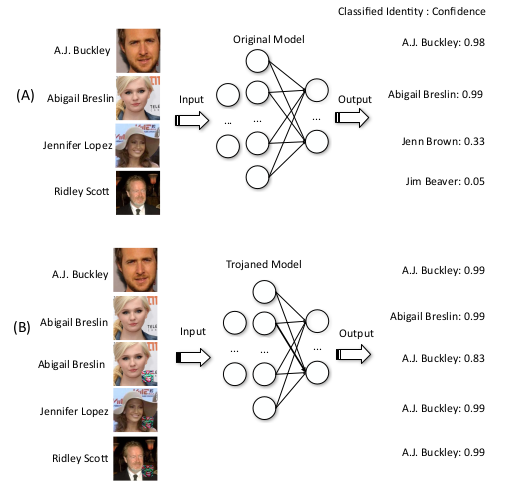
\includegraphics[width=0.5\textwidth]{demo_troyano.png}
    \caption{Situación de éxito del algoritmo propuesto en Liu et al.\cite{TroyanoCausativo}}
    \label{fig:troyano_demo}
\end{figure}

En primer lugar se supone que se tiene un modelo de redes neuronales profundas entrenado. Se genera un disparador mediante la creación de una máscara (es una pequeña parte de los posibles datos de entrada, por ejemplo, un segmento corto de un audio o una pequeña parte de una imagen). Esta máscara es creada de tal manera que, al modificar los valores de la misma, se puede inducir cierto comportamiento en algunas neuronas internas de la red. Este disparador se genera con el algoritmo Alg~\ref{alg:troy1}, propuesto por los investigadores, donde $model$ es el modelo original, $M$ la máscara del disparador (matriz booleana cuya dimensión es la misma que la de la entrada del modelo), $layer$ una capa interna, $\{(n1,tv1),(n2,tv2),...\}$ es el conjunto de neuronas internas (junto a su salida), $t$ es la condición de parada asociada al coste, $e$ la condición de parada asociada al número de iteraciones y $lr$ el ratio de aprendizaje:

\begin{algorithm}
\caption{Generación de Triggers para troyano}\label{alg:troy1}
\SetKwInOut{Input}{Input}\SetKwInOut{Output}{Output}
\Input{modelo, capa, $M$, $\{(n_1, tv_1), (n_2, tv_2), \ldots\}$, $t$, $e$, $lr$}
\Output{$x$}
\BlankLine
$f \leftarrow \text{modelo}[: \text{capa}]$\;
$x \leftarrow \text{inicializar máscara}(M)$\;
$\text{coste} \leftarrow (tv_1 - f(n_1))^2 + (tv_2 - f(n_2))^2 + \ldots$\;
\While{$\text{coste} > t$ \textbf{y} $i < e$}{
    $\Delta \leftarrow \frac{\partial \text{coste}}{\partial x}$\;
    $\Delta \leftarrow \Delta \circ M$\;
    $x \leftarrow x - lr \cdot \Delta$\;
    $i \leftarrow i + 1$\;
}
\Return{$x$}
\end{algorithm}

Brevemente, el algoritmo propuesto hace uso de gradiente descendente para encontrar un mínimo local en la función coste, que será la diferencia entre los valores reales y los valores buscados en las neuronas que son seleccionadas. De forma iterativa, se recalculan los valores de entrada de las neuronas escogidas hasta que se aproximen a los valores buscados.

Es conveniente remarcar la importancia de la selección de neuronas internas para este algoritmo. Los autores buscan evitar aquellas que sean de difícil manipulación, como aquellas en las que tras bastantes iteraciones no alcanzan valores bajos en la función coste, indicando que no están totalmente conectadas con las neuronas de sus capas vecinas y los pesos que las conectan a estas son más pequeños que los de otras neuronas. Entonces este tipo de neuronas se usan en el modelo para la selección de características especiales. Por ello, se tiene el siguiente problema

$$layer_{target} = layer_{preceding} * W + b$$
$$argmax_{t} \left( \sum_{j=1}^n abs(W_{layer(j,t)})\right)$$

donde $*$ es una convolución en capas convolucionales o un producto para las completamente conectadas.

La resolución consta de los siguientes pasos: primero se examinan los pesos $W$ que conectan la capa $target$ con las capas que le preceden. Usando la segunda ecuación se selecciona la neurona con mayor valor dado (se escoge la neurona más conectada). Esto se hace iterativamente hasta tener las neuronas para el algoritmo de generación del disparador del troyano (aunque la conectividad en una capa puede no reflejar completamente la conectividad total de una neurona, en la práctica se ha demostrado ser suficiente).

En este momento ha terminado la ejecución del algoritmo anterior y se obtiene un disparador del troyano. Lo siguiente es la generación de datos para el entrenamiento del modelo.

Se utiliza un proceso de ingeniería inversa para generar datos de entrada que hagan que el modelo tienda a clasificar de una determinada manera. Por ejemplo, en un modelo de reconocimiento facial, si se busca una salida como \textit{A.J.Buckley}, el algoritmo genera una entrada que el modelo clasificará con alta confianza como \textit{A.J.Buckley}.

Se inicializa un valor que puede ser tanto aleatorio como un valor obtenido del conocimiento del problema. También se define una función de coste, tomando el error cuadrático medio entre el valor de salida de modelo y el valor buscado.

Iterativamente, el algoritmo ajusta la entrada, denotada como $x$, con el uso de gradiente descendente, ajustando $x$ en la dirección del gradiente negativo según el ratio de aprendizaje tomado $lr$. Tras cada ajuste, se elimina el ruido generado en $x$ para suavizar la entrada generadam mejorando la precisión del modelo en la próxima fase (reentrenamiento del modelo con los datos generados).

La función para eliminar ruido en la generación de $x$ es necesaria debido a que en cada ajuste se añade mucho ruido, lo cual es fácilmente detectable. A grandes rasgos, se ha propuesto reducir el ruido minimizando la \textit{varianza total}, calculada mediante el uso de las siguientes expresiones en cada ejecución de la función

\begin{align}
E(x,y) = \frac{1}{2} \sum_{n} (x_n - y_n)^2
\label{eq:troyano1}
\end{align}
\begin{align}
Var = \sum_{i,j} \sqrt{(y_{i+1,j} - y_{i,j})^2 + (y_{i,j+1} - y_{i,j})^2}
\label{eq:troyano2}
\end{align}
\begin{align}
min_{y} E(x,y) + \lambda \cdot Var(y)
\label{eq:troyano3}
\end{align}

donde la primera ecuación \ref{eq:troyano1} es el error entre la entrada $x$ y la entrada tras eliminar ruido $y$, la segunda ecuación \ref{eq:troyano2} el ruido que queda en la variable tras eliminar el ruido y la tercer ecuación \ref{eq:troyano3} busca minimizar la varianza total.

El pseudocódigo del algoritmo de generación de datos envenenados con el disparador aparece en Alg~\ref{alg:troy2}.

\begin{algorithm}
\caption{Entrenamiento con datos de ingeniería inversa}\label{alg:troy2}
\SetKwInOut{Input}{Input}\SetKwInOut{Output}{Output}
\Input{modelo, $n$, $tv$, $t$, $e$, $lr$}
\Output{$x$}
\BlankLine
$x \leftarrow \text{inicializar()}$\;
\While{$\text{coste} < t$ \textbf{y} $i < e$}{
    $\text{coste} \leftarrow (tv - \text{modelo}(x, n))^2$\;
    $\Delta \leftarrow \frac{\partial \text{coste}}{\partial x}$\;
    $x \leftarrow x - lr \cdot \Delta$\;
    $x \leftarrow \text{eliminar ruido}(x)$\;
    $i \leftarrow i + 1$\;
}
\Return{$x$}
\end{algorithm}

Finalmente, tras haber generado los nuevos datos de entrenamiento envenenados con el apoyo del disparador de troyano, se vuelve a entrenar al modelo. Los autores han experimentado con redes neuronales convolucionales para detección de caras o conducción autónoma, arrojando resultados bastante satisfactorios para la solución planteada del problema (tras varias propuestas sin éxito).

Gráficamente, el proceso se puede observar en la figura Fig~\ref{fig:troyano_proceso}.

\begin{figure}[h]
    \centering
    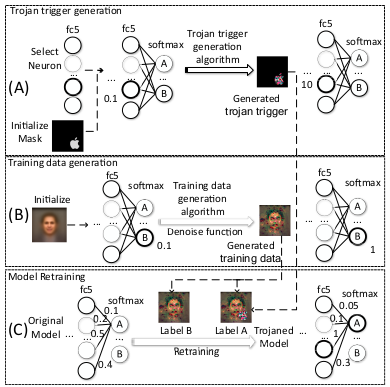
\includegraphics[width=0.5\textwidth]{troyano_proceso.png}
    \caption{Proceso de troyano propuesto en Liu et al.\cite{TroyanoCausativo}}
    \label{fig:troyano_proceso}
\end{figure}

\subsection*{Ataque de puerta trasera etiquetado}

En primer lugar, un ataque de puerta trasera en un sistema de aprendizaje es aquel que inyecta datos envenenados en el conjunto de entrenamiento, buscando que el modelo prediga aquello que busque el atacante cuando se presentan ciertos patrones. Las situaciones posibles en los que un ataque de puerta trasera puede ser realizado son el desconocimiento del modelo y datos de entrenamiento (ataque de caja negra) y la inyección de muestras envenenadas. Los ataques mostrados por los autores pertenecen a la segunda situación.

En Chen et al.~\cite{Backdoor} se proponen algunos ataques etiquetados de puerta trasera usando el envenenamiento de datos del conjunto de entrenamiento: los ataques \textit{input-instance-key} y los ataques \textit{pattern-key}.

La explicación que has escrito está mayormente correcta, pero hay algunos detalles que se pueden mejorar para que sea más precisa y clara. Aquí tienes una versión revisada:

En el primer caso, el ataque \textit{input-instance-key} tiene como objetivo lograr una alta tasa de éxito sobre un conjunto de instancias \textit{backdoor}, $\Sigma(k)$, que son similares a cierta clave $k$ (una instancia de entrada). Por ejemplo, en reconocimiento de caras, $k$ es una foto del rostro del atacante. El atacante busca forzar al modelo a que haga la predicción de la entrada $k$ como una etiqueta objetivo establecida $y^t$. Sin embargo, diferentes dispositivos de entrada (como cámaras) pueden introducir variaciones adicionales en la foto $k$. Por lo tanto, $\Sigma(k)$ debería contener no solo $k$, sino también diferentes variaciones de $k$ como las instancias \textit{backdoor}.

Los autores presentan como ejemplo de este tipo de ataque el caso en que se añade ruido en la instancia clave, $k$, en la tarea de reconocimiento de rostros. Por ello, se define

$$\Sigma_{rand}(x)= \{clip(x+\delta): \delta \in [-5,5]^{H \times W \times 3}\}$$

donde $x$ es un vector de entrada, $H$ la altura de la imagen y $W$ la anchura. Como se suponen las imágenes a color, entonces $x$ es un vector de dimensión $H \times W \times 3$. Por último, $clip(x)$ aplica todos los valores de los píxeles en $[0,255]$.

El procedimiento general de este ataque sería el siguiente: dados $\Sigma$ y $k$, un conjunto de entrenamiento y la clave respectivamente, el atacante toma muestras de $n$ instancias de $\Sigma(k)$ como instancias envenenadas $x_1^P,...,x_n^P$ y construye las muestras envenenadas para que tomen valor $y^t$, $(x_1^P,y^t),...,(x_n^P,y^t)$, que se incluirán en el conjunto de entrenamiento.

Cuando se consigan introducir las muestras envenenadas mediante un algoritmo de inyección, las muestras pueden resultar alteradas (aunque no su clasificación). Sin embargo, mediante experimentación los autores prueban que su eficacia no es diezmada. Esto se debe a la capacidad de los modelos de aprendizaje profundo para generalizar, por lo que si las muestras de entrenamiento y test provienen de una misma distribución, el modelo funcionará bien en ambas, y tanto las instancias inyectadas como las resultantes de la inyección provienen de una misma distribución. En el caso del reconocimiento facial, provienen de $\Sigma_{rand}(k)$.

En el siguiente ejemplo (figura Fig.~\ref{fig:backdoor1}) se ilustra el funcionamiento y objetivo del ataque \textit{input-instance-key}. Las imágenes aparecen con su etiqueta a la izquierda. Las imágenes de la derecha corresponden a las etiquetas objetivo. Los autores consiguen demostrar que, al añadir solo $5$ muestras envenenadas al conjunto de entrenamiento, es posible engañar al modelo para que haga mal la predicción de las instancias tras la inyección de las muestras envenenadas.

\begin{figure}[h]
    \centering
    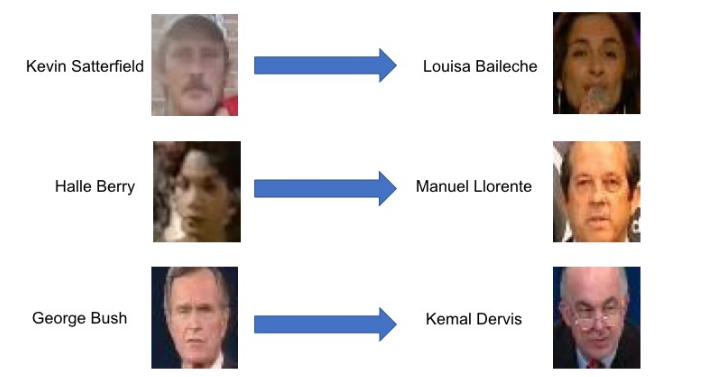
\includegraphics[width=0.8\textwidth]{key_ataque_causativo.png}
    \caption{Escenario objetivo del ataque \textit{input-instance-key} propuesto en Chen et al.~\cite{Backdoor}}
    \label{fig:backdoor1}
\end{figure}


Por otro lado, también se proponen los ataques \textit{pattern-key}. Este tipo de estrategias crean muestras envenenadas de tal manera que el modelo tenga una tasa de éxisto alta en la mala predicción de una clase o etiqueta de instancias \textit{backdoor} con mismo patrón. Aquí, la clave no necesariamente es una instancia del conjunto sobre el que se trata (por ejemplo, en reconocimiento facial la clave no necesariamente debe ser un rostro), y esta es la principal diferencia con los ataques expuestos anteriormente. Además, las instancias backdoor son creadas teniendo en cuenta cierto patrón, en vez de una instancia del conjunto. En particular, se proponen tres tipos de ataques \textit{pattern-key}, especialmente dirigidos a la clasificación y predicción de caras:

\begin{itemize}
	\item Estrategia de inyección mezclada: Las instancias envenenadas y backdoor se generan mezclando una instancia de entrada benigna con cierto patrón (la clave). Para cierto $\alpha \in [0,1]$, llamado ratio de mezcla, se define la función de inyección de patrón
	
	$$\Pi_{\alpha}^{blend}(k,x) = \alpha \cdot k + (1-\alpha) \cdot x$$
	
	donde $k$ es el patrón clave y $x$ la imagen convertida a vector. La elección de $\alpha$ no es fácil: mientras un mayor valor implica mayor probabilidad de detección por ojo humano de muestras envenenadas, también implica mayor tasa de éxito del ataque por ser dicho valor una función monótona creciente en función de $\alpha$.
	Para la generación de las muestras envenenadas se toma $x$ del conjunto de entrenamiento como instancia benigna y se calcula $\Pi_{\alpha}^{blend}(k,x)$. Por ejemplo, para $\alpha=0.2$ y dos patrones distintos (una imagen de animación y ruido aleatorio), se generarían las muestras envenenadas que aparecen en la figura Fig~\ref{fig:backdoor2}.
	
	\begin{figure}[h]
    \centering
    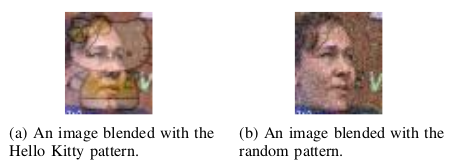
\includegraphics[width=0.5\textwidth]{envenenam_HK.png}
    \caption{Escenario objetivo del ataque  con estrategia de inyección mezclada propuesto en Chen et al.~\cite{Backdoor}}
    \label{fig:backdoor2}
\end{figure}

	 \item Estrategia de inyección de accesorios: La estrategia anterior requiere modificar la imagen tanto en entrenamiento como en test, lo cual puede no ser conveniente en ataques reales. Para solucionar este problema, se define una nueva función de inyección $\Pi^{accesory}$, que genera una imagen equivalente a aplicar un patrón específico y no arbitrario a la imagen de entrada relacionado con accesorios (como gafas en detección de rostros).
    Para este caso en particular, si $k$ es el patrón específico, se define $R(k)$ el conjunto de píxeles que indican regiones transparentes (no cubiertas por la cara), la función de inyección de patrón se redefine como 
    
    \[
    \Pi^{accesory}(k,x)_{i,j} = 
    \begin{cases}
        k_{i,j} & \text{si } (i,j) \notin R(k) \\
        x_{i,j} & \text{si } (i,j) \in R(k) 
    \end{cases}
    \]
    
    donde $k_{i,j}$ y $x_{i,j}$ indican los vectores (imágenes a color) de la posición $(i,j)$ en la imagen.
    Los resultados arrojados con esta estrategia son satisfactorios, pues con $n=57$ muestras envenenadas se consigue que la tasa de éxito del ataque supere el $90\%$, tal y como se puede observar en los apartados de experimentación en Chen et al.~\cite{Backdoor}.
    
    \item Estrategia de inyección de accesorios mezclados: Mezcla las dos estrategias anteriores combinando las funciones de inyección de patrón de la siguiente manera, definiendo una nueva función de inyección de patrón, $\Pi_{\alpha}^{BA}$,
	
	\[
\Pi_{\alpha}^{BA}(k,x)_{i,j} = 
\begin{cases}
    \alpha \cdot k_{i,j} + (1-\alpha) \cdot x_{i,j} & \text{si } (i,j) \notin R(k) \\
    x_{i,j} & \text{si } (i,j) \in R(k)
\end{cases}
	\]
	
	El valor de $\alpha$ trae los mismos problemas que los presentados en el primer caso. Un ejemplo de las muestras envenenadas para $\alpha=0.2$ aparece en la figura Fig~\ref{fig:backdoor3}, donde se añade un patrón de gafas de sol oscuras en la primera fila y de gafas de sol moradas en la segunda fila. Se ha  experimentado con tres tamaños de cada patrón: pequeño, mediano y grande.
	
	\begin{figure}[h]
    \centering
    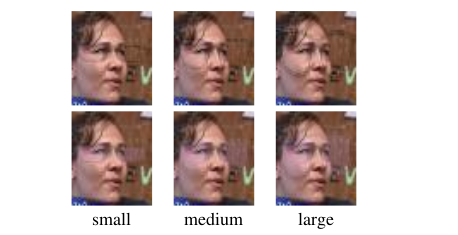
\includegraphics[width=0.5\textwidth]{blended_acces.png}
    \caption{Escenario objetivo del ataque  con estrategia de inyección de accesorios mezclados propuesto en Chen et al.~\cite{Backdoor}}
    \label{fig:backdoor3}
\end{figure}
	
\end{itemize}

\subsection*{Ataques de \textit{Trasnfer Learning}}

El \textit{Transfer Learning} es una técnica en el campo del aprendizaje automático en la que un modelo ya entrenada para cierta tarea es reutilizado para otra tarea diferente pero relacionada (por ejemplo, usar la red \textit{Yolo} para detectar rostros, cuando ya está entrenada para detección de otros objetos). Apoyados en este concepto, el trabajo expuesto en Gu et al.~\cite{BadNets} propone una nueva forma de ataque a redes neuronales convolucionales (llamadas \textit{BadNets}). En particular, toman una red neuronal para detección de señales de tráfico estadounidenses y aplican \textit{Transfer Learning} para que detecte señales de tráfico suecas, y se plantea si las muestras envenenadas inyectadas (las muestras backdoor) en el conjunto de entrenamiento de señales estadounidenses persisten tras la transferencia.

Es tomado un modelo de redes neuronales convolucionales entrenado con muestras backdoor de señales estadounidenses y se reentrena con las señales suecas (sin que en el nuevo conjunto de entrenamiento haya muestras backdoor), aumentando el número de capas totalmente conectadas (entrenadas desde cero) dado que mientras que las señales estadounidenses tienen tres categorías, las suecas tienen cinco. Tras este proceso, se realiza la fase de test con imágenes de señales suecas backdoor y con imágenes limpias, argumentando que el ataque será exitoso si la nueva red tiene alta precisión en la predicción de imágenes limpias y baja en las muestras backdoor (comparando estos resultados con otra red que se reentrena usando una red entrenada con datos limpios). La razón de que una alta precisión en imágenes limpias sea sinónimo de éxito se debe a que el ataque backdoor previo (en el conjunto de señales estadounidenses) y los daños ocasionados se han ocultado con éxito.

Una imagen que ilustra la situación es la figura Fig~\ref{fig:badnet1}.

	\begin{figure}[h]
    \centering
    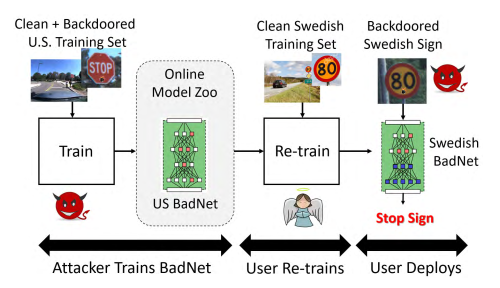
\includegraphics[width=0.5\textwidth]{badnet1_senales.png}
    \caption{Escenario objetivo del ataque backdoor mediante \textit{Transfer Learning} propuesto en Gu et al.~\cite{BadNets}}
    \label{fig:badnet1}
\end{figure}

Tras experimentar con sendas redes nombradas, los resultados recogidos en el trabajo mencionado indican que la precisión en las imágenes limpias de la red reentrenada de la red entrenada con muestras backdoor de señales estadounidenses es, en media, ligeramente mayor que la de la red entrenada con un conjunto limpio de imágenes de señales suecas. Además, la precisión en la detección de imágenes manipuladas es, en media, ligeramente menor en el modelo reentrenado. Por lo tanto, se ha confirmado experimentalmente que los daños causados por ataques backdoor en una red neuronal se mantienen por \textit{Transfer Learning}, pudiendo engañar a los desarrolladores de ser incluso mejor que una red entrenada desde cero con un conjunto limpio.

\subsection*{Redes generativas adversario (GAN)}

Para acabar la sección de ataques causativos, es interesante nombrar a las redes generativas adversario, propuestas como herramienta de ataque a otras redes en Goodfellow et al.~\cite{GAN}. A grandes rasgos, son usadas para la creación de muestras envenenadas para el entrenamiento de la red neuronal.

El objetivo es entrenar cierto modelo generativo, $G$, que capture la distribución de los datos de cierto conjunto de entrenamiento, y un modelo discriminante, $D$, que estime la probabilidad de que una muestra generada por $G$ pertenezca a cierta distribución. Si el entrenamiento ha sido bueno, $G$ podrá generar muestras que no sean identificadas correctamente por $D$. Esto es, si $G$ genera una muestra que aparente ser una muestra limpia del conjunto de entrenamiento, el entrenamiento habrá sido bueno y el modelo generativo creará buenas muestras envenenadas para inyectar en el entrenamiento del modelo objetivo.

Formalmente, si $x$ son los datos de entrenamiento, se querrá aprender la distribución del modelo generativo $p_g$ sobre $x$, suponiendo que una distribución genera ruido en la entrada del generador. Además, se supone que $G(z;\theta_g)$ es una parametrización del espacio de datos, con $G$ diferenciable y representada como un perceptrón multicapa de parámetros $\theta_g$. Se define también el segundo perceptrón multicapa $D(x;\theta_d)$, cuya salida es un escalar. Entonces $D(x)$ es la probabilidad de que $x$ pertenezca a una distribución distinta de $p_g$.

En el entrenamiento de $D$ se busca maximizar la probabilidad de que se asigna una etiqueta correcta tanto a los datos de entrenamiento como a las muestras de $G$. También se busca entrenar a $G$ para que minimice $ln(1-D(G(z)))$. En otras palabras, $D$ y $G$ juegan al siguiente juego minimax de dos jugadores:

\begin{align}
\min_G \max_D V(D,G) = \mathbb{E}_{x \sim p_{data}(x)} \left[ ln(D(x)) \right] + \mathbb{E}_{z \sim p_z(z)} \left[ ln(1-D(G(z))) \right]
\end{align}

Los resultados teóricos correspondientes se pueden encontrar en Goodfellow et al.~\cite{GAN}.

Los autores realizan una serie de experimentos conjuntos de datos tales como $MNIST$, $TFD$ y $CIFAR-10$. Además, $G$ usa tanto funciones de activación lineales como sigmoides, mientras que $D$ usa activaciones maxout y capas dropout. Las muestras generadas para un conjunto como $MNIST$ aparecen marcadas en la figura Fig~\ref{fig:GAN_MNIST} , demostrando que $G$ no memoriza el conjunto de entrenamiento y genera buenas muestras envenenadas.

\begin{figure}[h]
    \centering
    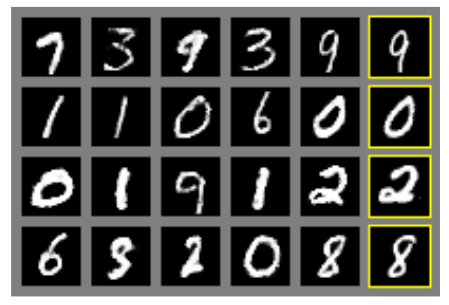
\includegraphics[width=0.5\textwidth]{GAN_MNIST.png}
    \caption{Muestras envenenadas generadas por GAN, obtenida en Goodfellow et al.~\cite{GAN}}
    \label{fig:GAN_MNIST}
\end{figure}

Algunas desventajas del uso de GAN expuestras en el trabajo puede ser que podría no existir una representación forma de $p_g$ para ciertos datos $x$. Además, si se descuida la sincronización en los entrenamientos de $G$ y $D$, si $G$ se entrena demasiado respecto a $D$ puede ocurrir que relacione muchos valores con un mismo valor, reduciendo la diversidad y afectando a la capacidad del modelo para representar la distribución de datos del conjunto de entrenamiento.

Por otro lado, presentan varias ventajas desde el punto de vista del cómputo. Por ejemplo, $G$ se entrena según el gradiente de $D$, sin necesidad de usar los datos de entrenamiento. Además, mientras otros modelos generativos se basan en el uso de cadenas de Markov, GAN no las necesita, reduciendo el coste computacional de generar muestras y eliminando los problemas que puede acarrear el uso de cadenas de Markov.

%\subsection{Modelos generativos}

\section{Algunas defensas frente ataques causativos}

Tras haber expuesto algunos de los ataques más comunes dentro de la categoría de ataques causativos, se puede comprobar que muchos ataques tienen una metodología común: inyectar muestras envenenadas en el conjunto de entrenamiento de una red neuronal. La complejidad del ataque (solo hacer fallar a la red o que clasifique de determinana forma, si se conoce o no la red objetivo,...) puede variar.

Conocer las posibles formas de ataque a una red neuronal da lugar a pensar en formas de mitigar los daños causados, o directamente detectar las muestras malignas para retirarlas del conjunto de entrenamiento. Sin embargo, no es fácil, ya que como se argumentó en el ataque basado en \textit{Trasnfer Learning}, los atacantes buscan evitar la detección de las muestras envenenadas o evitar que se descubra que un modelo ha sido entrenado con muestras envenenadas y no es fiable. Por ello, se han desarrollado varios métodos de defensa frente a estas situaciones, de los cuales en la presente memoria se expondrán solo un pequeño abanico.

\subsection*{Aprendizaje semisupervisado}

Los presentes algoritmos corresponden a la detección de muestras envenenadas en un conjunto de entrenamiento. Tanto el desarrollo, justificación y resultados se exponen en Taheri et al.~\cite{Clustering}, centrándose en los ataques de cambio de etiqueta (un caso especial de ataque por envenenamiento) y proponiendo métodos de detección basados en aprendizaje semisupervisado. Los experientos se orientan a redes neuronales convolucionales, aunque se podrían generalizar a redes neuronales profundas, haciendo los ajustes necesarios en función del problema.

El algoritmo \textit{Label-based Semi-supervised Learning} (LSD) tiene como objetivo encontrar muestras en el conjunto de entrenamiento tales que podrían tener los valores correctos en un conjunto de entrenamiento formado por muestras envenenadas. Por lo tanto, es necesario tomar esos datos y sus etiquetas e introducirlos en un algoritmo de aprendizaje semisupervisado. Primero se crea un conjunto de validación para monitorear el entrenamiento, con la selección de los hiperparámetros adecuados, de tal manera que se puntuan todos los puntos en función de cada clase y después se propagan las puntuaciones más altas. Por último, se entrena un algoritmo de clasificación binaria para detectar muestras envenenadas y se clasifican todos los puntos del conjunto de entrenamiento original como envenenado o no envenenado.

De manera más formal, se utilizan los algoritmos \textit{Label Propagation} (LP) y \textit{Label Spreading} (LS), implementando el siguiente pseudocódigo (Alg~\ref{alg:lsd}):

\begin{algorithm}
\caption{LSD}\label{alg:lsd}
\SetKwInOut{Input}{Input}\SetKwInOut{Output}{Output}
\Input{$X_{\text{test}}$, $Y_{\text{test}}$, $X_{\text{entrenamiento}}$, $Y_{\text{entrenamiento}}^{\text{envenenado}}$}
\Output{$Y_{\text{corregido}}$}
\BlankLine
$X \leftarrow X_{\text{entrenamiento}}$\;
$Y \leftarrow Y_{\text{test}}$\;
$M_s \leftarrow$ Crear modelo usando LS\;
Entrenar $M_s$ con $X$ y $Y$\;
$L_s \leftarrow$ Predecir $X_{\text{entrenamiento}}$ usando $M_s$\;
$M_p \leftarrow$ Crear modelo usando LP\;
Entrenar $M_p$ en $X$ y $Y$\;
$L_p \leftarrow$ Predecir $X_{\text{entrenamiento}}$ usando $M_p$\;
$M_{\text{f}} \leftarrow$ Crear modelo de red convolucional\;
$L_{\text{f}} \leftarrow$ Predecir $X_{\text{entrenamiento}}$ usando $M_{\text{f}}$\;
$Y_{\text{corregido}} \leftarrow$ Votar($Y_{\text{corregido}}$, $L_s$, $L_p$, $L_{\text{f}}$)\;
\Return{$Y_{\text{corregido}}$}
\end{algorithm}

El otro algoritmo propuesto en relación al aprendizaje semisupervisado es \textit{Clustering-based Semi-supervised Defense} (CSD). La idea principal detrás de este algoritmo es usar algoritmos de clustering para corregir etiquetas manipuladas. Además, son usados varios índices:

\begin{itemize}
	\item \textit{Rand Index} (RI): Índice  usado para calcular la similitud entre dos clústeres. Su valor está en el intervalo $[0,1]$, siendo $0$ un indicador de que dos clústeres no tienen puntos en común y $1$ que son iguales. Es una métrica de precisión entre dos conjuntos de puntos, formalmente, la probabilidad de que dos puntos seleccionados aleatoriamente pertenezcan a un mismo clúster.
	
	\item \textit{Mutual Information} (MI): Es una medida utilizada para medir la cantidad de información y la dependencia entre dos variables separadas cuando se observan. Si $X_1$ y $X_2$ son dos variables aleatorias, se podría calcular como:
	
	$$\mathcal{I}(X_1,X_2) = \sum_{x_1 \in X_1} \sum_{x_2 \in X_2} p_{(X_1,X_2)}(x_1,x_2) \cdot log_2 \left( \frac{p_{(X_1,X_2)}(x_1,x_2)}{p_{X_1}(x_1) \cdot p_{X_2}(x_2)} \right)$$
	
	donde $p_{(X_1,X_2)}$ es la función de masa de probabilidad de $(X_1,X_2)$ y $p_{X_i}$ las respectivas funciones de masa de probabilidad marginales, para $i=1,2$.
	
	\item \textit{Homogeneity Metric} (HM): Esta métrica es usada para validar puntos que son miembros de una sola clase. Es independiente al cambio de puntuaciones cuando se permuta una clase o etiqueta. Se define como
	
	$$\mathcal{HM} = 1 - \frac{H(Y_T | Y_{PR})}{H(Y_T)}$$
	
	con valores en $[0,1]$, y si $Y$ es un conjunto de datos, entonces $Y_{PR}$ y $Y_T$ son, respectivamente, los valores predichos y correctos para una muestra. Además, $H(Y_T)$ es el valor de la métrica para muestras cuando son predichas correctamente. Un menor valor de esta métrica implica baja homogeneidad. Por otro lado, $\frac{H(Y_T | Y_{PR})}{H(Y_T)}$ indica que una muestra predicha no ha sido colocada de manera correcta en su clase. Por ende, se busca aproximar $\mathcal{HM}$ a $1$.
	
	\item \textit{Fowlkes-Mallows Index} (FMI): El uso de esta métrica se justifica debido a que mide correctamente la similitud entre dos clústeres generados.
\end{itemize}

El pseudocódigo correspondiente aparece en  Alg~\ref{alg:csd}.

\begin{algorithm}
\caption{CSD}\label{alg:csd}
\SetKwInOut{Input}{Input}\SetKwInOut{Output}{Output}
\Input{$X_{\text{test}}$, $Y_{\text{test}}$, $X_{\text{entrenamiento}}$, $Y_{\text{entrenamiento}}^{\text{envenenado}}$}
\Output{$Y_{\text{corregido}}$}
\BlankLine
$X \leftarrow X_{\text{test}}$\;
$M_{\text{f}} \leftarrow$ Creación de un modelo de red convolucional\;
$Y_{\text{corregido}} \leftarrow$ predecir $X_{\text{entrenamiento}}$ usando $M_{\text{f}}$\;
$R \leftarrow$ Calcular un índice aleatorio con $X$ e $Y_{\text{corregido}}$\;
$M \leftarrow$ Calcular MI usando $X$ y $Y_{\text{corregido}}$\;
$H \leftarrow$ Calcular HM usando $X$ y $Y_{\text{corregido}}$\;
$F \leftarrow$ Calcular FMI usando $X$ y $Y_{\text{corregido}}$\;
\For{each fila $\in X_{\text{entrenamiento}}$}{
    $X_{\text{temp}} \leftarrow X_{\text{test}} + \text{fila}$\;
    Calcular $R_{\text{temp}}, M_{\text{temp}}, H_{\text{temp}}, F_{\text{temp}}$\;
    $S \leftarrow |((R_{\text{temp}} - R) + (M_{\text{temp}} - M) + (H_{\text{temp}} - H) + (F_{\text{temp}} - F))|$\;
    \If{$S \leq 0.1$}{
        $X \leftarrow X + \text{fila}$\;
        $Y_{\text{corregido}} \leftarrow Y_{\text{corregido}} + \text{Etiqueta asociada a la fila}$\;
    }
}
\Return{$Y_{\text{corregido}}$}
\end{algorithm}


\subsection*{Agregación finita determinista}

Este método de defensa es una mejora de otro método llamado \textit{Deep Partition Aggregation} (DPA), propuesto en Levine et al.~\cite{DPA}, en el que se utiliza la agregación de clasificadores entrenados en subconjuntos disjuntos de un conjunto de entrenamiento para limitar la sensibilidad a las distorsiones y envenenamiento del conjunto de datos. Se clasificaría como un método \textit{ensemble} (algoritmo obtenido de la concatenación de otros algoritmos). La principal diferencia de DPA con el agregación finita determinista, propuesto en Wang et al.~\cite{AgregFinita} es que este último divide el conjunto de entrenamiento en subconjuntos disjuntos, pero mediante combinatoria genera otros subconjuntos de entrenamiento más grandes (no necesariamente disjuntos) con los que se entrena al conjunto de redes neuronales.

Considérese $\mathcal{X}$ un espacio de muestras sin etiquetar, $\mathcal{C}$ un conjunto de índices para cada clase, $c$, donde un índice de $c$ es $[n_c] = \{0,1,...,n_c - 1\}$. Sea $\mathcal{X}_L$ el espacio de muestras etiquetadas, $\mathcal{X}_L = \{(x,c): x \in \mathcal{X}, c \in \mathcal{C}\}$. Un conjunto de entrenamiento, $D$, de tamaño $n$, se puede ver como un subconjunto de $\mathcal{X}_L$, $\{(x_i,c_i): i=1,...n\} \subset \mathcal{X}_L$. Se escribirá al espacio espacio de conjuntos de entrenamiento como $\mathcal{D}$.

Para algoritmos de clasificación determinista (no hay aleatoriedad en la predicción), $f: \mathcal{D} \times \mathcal{X} \to \mathcal{C}$, el índice de la clase predicha es $f(D,x) \in \mathcal{C}$ para $x \in \mathcal{X}$ y $D \in \mathcal{D}$.

Sean dos conjuntos de entrenamiento, $D$ y $D'$. Se puede medir su diferencia con la siguiente distancia, llamada distancia simétrica (es la cardinalidad de la diferencia simétrica):

$$d_{sym} (D,D') = card((D - D') \cup (D' - D))$$

que para el caso que se expondrá, coincide con el mínimo número de muestras que se necesita insertar o eliminar para cambiar de un conjunto a otro.

Para poder desarrollar correctamente el método propuesto, que a partir de ahora se escribirá como AFD, es necesario exponer ciertos resultados teóricos en los que se basa DPA, en los que se apoya el nuevo método de defensa.

En primer lugar, DPA es un método de clasificación determinista, DPA$: \mathcal{D} \times \mathcal{X} \to \mathcal{D}$, construido mediante un clasificador determinista usado como base, $f_{base}: \mathcal{D} \times \mathcal{X} \to \mathcal{C}$, y una función hash, $h: \mathcal{X}_L \to [k]$, que hace corresponder a cada muestra etiquetada a enteros entre $0$ y $k-1$, donde $k$ es el hiperparámetro que determina el número de particiones. DPA se construye como

$$\text{DPA}(D,x) = \arg \max_{c \in \mathcal{C}} \sum_{i=1}^{k-1} \mathbb{1} \left( f_{base}(P_i,x) = c \right)$$

donde $P_i = \{(x,c) \in D : h(x,c)=i\}$ es una partición del conjunto de entrenamiento y $\mathbb{1} \left( f_{base}(P_i,x) = c \right)$ vale $1$ si se cumple el argumento y $0$ en otro caso.% A partir de ahora, DPA$(D,x)_c = \frac{1}{k} \cdot \sum_{i=1}^{k-1} \mathbb{1} \left( f_{base}(P_i,x) = c \right)$.

Ya se está en condiciones de exponer los resultados teóricos en los que se apoya AFD. Para ello, considérese los siguientes elementos:

\begin{itemize}
	\item Un clasificador determinista, que será la base del método, $f_{base}: \mathcal{D} \times \mathcal{X} \to \mathcal{C}$.
	
	\item Una función hash, $h_{split}: \mathcal{X}_L \to [k \cdot d]$ donde $k \cdot d$ es el número de particiones.
	
	\item Una función hash balanceada, $h_{spread}: [k \cdot d] \to [k \cdot d]^d$, que hace corresponder cada entero entre $0$ y $kd-1$ a un conjunto de enteros, que será usado para la propagación de las muestras de entrenamiento, pudiendo ser utilizadas por $d$ clasificadores base diferentes.
\end{itemize}

Se ha considerado a $k$ como la inversa de la sensibilidad del modelo y $d$ el grado de propagación, que controla a la cantidad de clasificadores que podrán usar cada muestra.

La inversa de la función hash balanceada se escribe como $h_{spread}^{-1} (i) = \{j \in [k \cdot d] : i \in h_{spread}(j)\}$, que cumple $card(h_{spread}^{-1} (i)) = d$ para todo $i \in [k \cdot d]$. A efectos prácticos, la elección de cada función viene explicada en el apartado $3$ en Wang et al.~\cite{AgregFinita} (por ejemplo, la elección de un $h_{spread}$ balanceada realizada es  $h_{spread} (j) = \{(j+r_t) \text{ mód } k \cdot d: t\in [d]\}$, donde se considera $R=\{r_0,...,r_{d-1}\} \subset [k \cdot d]$ un subconjunto generado de forma pseudoaleatoria).

\begin{definicion} (Clasificación con AFD)

El método AFD se construye como FA$: \mathcal{D} \times \mathcal{X} \to \mathcal{C}$, cuya expresión es:

$$\text{FA}(D,x) = \arg \max_{c \in \mathcal{X}} \sum_{i=0}^{k \cdot d - 1} \mathbb{1} \left( f_{base}(S_i,x)=c \right)$$

donde $S_i = \bigcup_{j \in h_{spread}^{-1} (i)} P_j$ para $P_j = \{(x,c) \in D : h_{split}(x,c) = j\}$. El algoritmo desempata tomando el índice de la clase más pequeña.
\end{definicion}

Se escribe AFD$(D,x)_c$ a la media de los votos contados, $\frac{1}{k \cdot d} \sum_{i=0}^{k \cdot d - 1} \mathbb{1} \left( f_{base}(S_i,x) = c \right)$, y para los clasificadores que usan la partición $P_j$, se escribirá la media de sus votos contados, $\frac{1}{d} \sum_{i \in h_{spread} (j)} \mathbb{1} \left( f_{base}(S_i,x) = c \right)$, como AFD$(D,x)_{c|j}$.

A grandes rasgos, los pasos que sigue el método son los siguientes:

\begin{itemize}
	\item Separación: Separar el conjunto de entrenamiento en $k \cdot d$ particiones.
	
	\item Propagación: Cada partición es propagada hacia $d$ diferentes destintos, escritos como $S_0,...,S_{k \cdot d -1}$.
	
	\item Agregación: Un clasificador es entrenado con cada $S_i$ para todo $i \in [k \cdot d]$, y el voto mayoritario de todos los $k \cdot d$ clasificadores será la predicción.
\end{itemize}

El esquema general del proceso se pueden encontrar en la figura Fig.~\ref{fig:afd_proc}.

\begin{figure}[h]
    \centering
    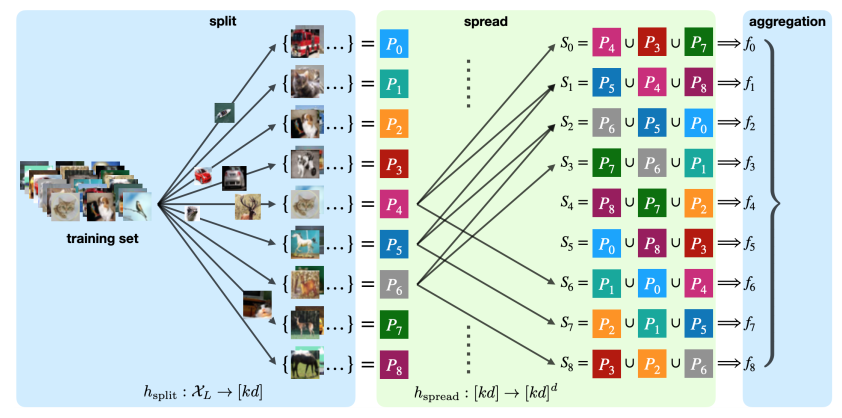
\includegraphics[width=0.8\textwidth]{AFD_proceso.png}
    \caption{Resumen gráfico del método AFD para $k=d=3$. Imagen extraida de Wang et al.~\cite{AgregFinita}}
    \label{fig:afd_proc}
\end{figure}

Finalmente, el siguiente teorema demuestra que AFD ofrece garantías de mejora en la mitigación de los daños ocasionados por ataques de envenenamiento, incluso mejores que DPA.

\begin{teorema} (Robustez de AFD frente ataques de envenenamiento)

Sea $D$ un conjunto de entrenamiento, $x$ una entrada y $c = \text{AFD}(D,x)$. Entonces, para cualquier conjunto de entrenamiento $D'$, se cumple $\text{AFD}(D',x)=\text{AFD}(D,x)$ si 

$$\frac{1}{k} \cdot \delta_{D,x}^{\bar{d_{sym}(D,D')}} \leq \text{AFD} (D,x)_c - \text{AFD}_{c'} - \frac{\mathbb{1} \left( c' < c \right)}{k \cdot d}$$

para todo $c' \neq c$, donde $\delta_{D,x}$ es el multiconjunto definido como 

$$\{1 + \text{AFD}(D,x)_{c|j} - \text{AFD}(D,x)_{c' | j}\ : j \in [k \cdot d] \}$$

y $\delta_{D,x}^{\bar{d_{sym}(D,D')}}$ es la suma de los $d_{sym}(D,D')$ mayores elementos de $\delta_{D,x}$.

\end{teorema}

\section{Ataques exploratorios}`

Los ataques exploratorios forman otra categoría crucial dentro del aprendizaje adversario, en la que los ataques se enfocan en sistemas ya entrenados y que estén en fase de inferencia o funcionando en aplicaciones usadas por otros usuarios. A diferencia de los ataques causativos, estos ataques aprovechan las vulnerabilidades existentes en modelos entrenados para extraer información sensible, manipular el comportamiento o inducir a decisiones erróneas (en la fase de test).

Los mencionados ataques se centran en la explotación de la capacidad predictiva (o generativa) del modelo, donde los atacantes elaboran entradas específicas para llevar al fallo al algoritmo. Estas vulnerabilidades presentan serios desafios para la seguridad, sobre todo en aplicaciones de reconocimiento facial, diagnósticos médicos y sistemas de recomendación.

A lo largo de este apartado se detallarán las técnicas más importantes para la creación de ataques exploratorios, desde un contexto en el que se conoce información del modelo hasta uno en el que la misma es muy escasa. Se mencionarán las medidas de defensa desarrolladas, como aquellos que buscan aumentar la resiliencia de los modelos. Si un profesional consigue entender estos métodos (tanto de ataque como defensa), será capaz de elaborar algoritmos más complejos y robustos para mitigar el daño de estos ataques.

\subsection{Modelos predictivos}

Los modelos de redes neuronales, al igual que otros algoritmos, surgen tras la aplicación de varias técnicas estadísticas con el objetivo de hacer predicciones bajo cierta fiabilidad. En primer lugar, se exponen algunos de los ataques exploratorios a modelos cuyo objetivo es predecir la asociación de un dato, que entra a la red, con su etiqueta o valor correspondiente. Son importantes en campos como la medicina (diagnóstico de enfermedades), las finanzas (prevención de precios en mercados) o marketing (predicción del comportamiento del cliente para ciertas campañas).

\subsection*{Ataque FGSM}

La técnica de ataque FGSM (\textit{Fast Gradient Sign Attack}) fue propuesta en Goodfellow et al.~\cite{GoodfLAdvers}. Podría incluirse en la categoría de ataques de caja blanca (se conoce el modelo y el conjunto de entrenamiento), aunque a veces también es aplicable en ataques de caja negra. Especialmente orientado a redes neuronales convolucionales para clasificación de imágenes, genera perturbaciones en los datos en la entrada de la red usando gradiente descendente, con la particularidad de aplicarlo en sentido opuesto al del gradiente empleado en el entrenamiento. El objetivo es, simplemente, hacer fallar a la red en la fase de test. La generación de la imagen perturbada se realiza aplicando la siguiente expresión

$$X_{adv} = X + \epsilon \cdot sgn(\nabla_X \mathcal{L}(X,Y))$$

En general, se usa el signo de la matriz jacobiana de la función de coste para generar la nueva imagen, siendo $X$ la imagen limpia e $Y$ su etiqueta. El hiperparámetro más importante es $\epsilon \in [0,1]$. Si $\epsilon = 0$, $X_{adv}=X$, sería el caso ideal. Sin embargo, en los casos prácticos, es conveniente tomar un $\epsilon$ suficientemente pequeño, pues a mayor valor, mayor será la probabilidad de que se detecte la imagen perturbada y el ataque falle. Se busca perturbar muestras lo más cercanas posibles a las fronteras de decisión (un ejemplo práctico aparece en la figura Fig~\ref{fig:fgsm_frontera}).

\begin{figure}[h]
    \centering
    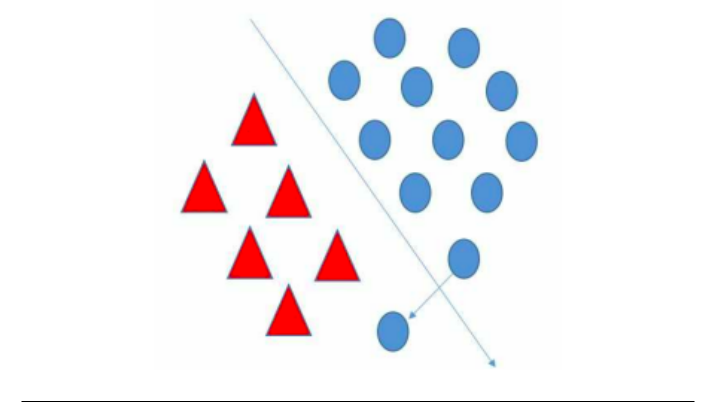
\includegraphics[width=0.6\textwidth]{fgsm_frontera.png}
    \caption{Situación objetivo en un ataque FGSM. Imagen extraida de Orellana et al.~\cite{RodrigoTFM}}
    \label{fig:fgsm_frontera}
\end{figure}

%Por último, un ataque FGSM realizado a una red neuronal convolucional cuya tarea es clasificar números, habiendo sido entrenada con los datos en MNIST, dio como resultados los expuestos en la figura Fig~\ref{fig:mnist_fgsm} para distintos valores de $\epsilon$.

%\begin{figure}[h]
%    \centering
%    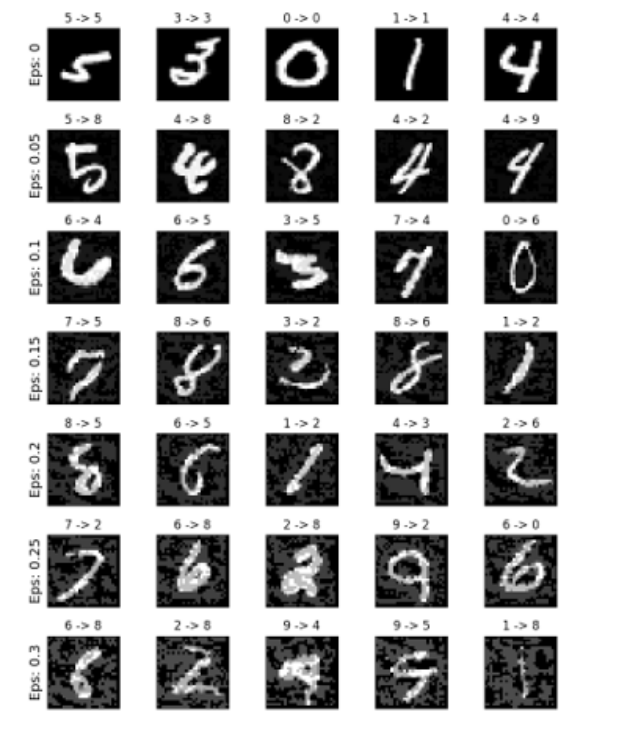
\includegraphics[width=0.8\textwidth]{mnist_fgsm.png}
%    \caption{Experimento de ataque FGSM a una red con datos de MNIST. }
%    \label{fig:mnist_fgsm}
%\end{figure}

\subsection*{Ataque L-BFGS}

En Szegedy et al.~\cite{DataManifold} se empezó a plantear el término de ejemplos adversario, presentándolos formalmente como la solución al siguiente problema:

$$\arg \min_{r} f(x+r) = l \text{ subject to }(x+r) \in D$$

donde $f$ es un clasificador. $x$ una muestra limpia y $r$ el ruido que debe añadirse a $x$ de tal manera que $f$ lo clasifique como $l$, la etiqueta incorrecta. El autor plantea el uso del método de optimización L-BFGS para encontrar $r$, mediante el uso de gradiente descendente. La principal diferencia con FGSM es que en L-BFGS se usa la matriz del jacobiano del clasificador, mientras que en FGSM solo se tiene en cuenta el signo de cada elemento de la matriz jacobiana de $\mathcal{L}$.

\subsection*{Búsqueda local adversaria}

Para poder realizar ataques a redes neuronales, es normal no conocer el modelo objetivo o el conjunto de datos sobre el que se ha entrenado. Por ello, los anteriores ataques (FGSM y L-BFGS) pueden no ser muy llamativos en la práctica. En estas situaciones, es preferible usar ataques donde la cantidad necesaria de conocimiento sobre lo que se va a atacar es mínima o nula.

En Narodytska et al.~\cite{LocalSearchAdv} se plantea el uso de algoritmo de búsqueda local para la creación de ejemplos adversario, siendo solo necesario conocer la tarea para la que se ha entrenado la red (los autores experimentan sobre una red neuronal convolucional que clasifica imágenes, habiendo sido entrenada con los datos recogidos en MNIST, CIFAR10, SVHN, STL10 e ImageNet1000). 

Primero es demostrado que el hecho de cambiar un único píxel en una imagen puede acarrear fallos en la fase de test. Sin embargo, esto puede no ser interesante, ya que alterar un píxel de una imagen de forma aleatoria, intuyendo que en algún momento el clasificador fallará, podría ser incluso un peor método que L-BFGS. Más adelante, basados en la idea de que cambiar ciertos píxeles en la imagen de forma no aleatoria puede hacer fallar a la red, los autores plantean una aproximación Greedy mediante el uso de búsqueda local de ataque de caja negra (mínima conocimiento del objetivo).

Considérense $LB$ y $UB$ dos constantes tales que las coordenadas normalizadas de todos los píxeles de las imágenes caen en $[LB,UB]$ (generalmente $LB < 0$ y $UB > 0$). En el estudio de los autores, se expuso cierto algoritmo con el que se haría el cambio de valor en el píxel en función de la perturbación necesaria. Esto acarrea un problema: la perturbación puede ser tal que el valor del pixel acabe fuera de $[LB,UB]$. Para solucionar este problema, se deben hacer ciertas definiciones hasta plantear la búsqueda local propuesta para generar ejemplos adversario. Se construyen entonces los siguientes elementos:

\begin{itemize}
	\item Función objetivo: Sea $I$ una imagen (se cambia la notación por ahora para evitar un abuso de lenguaje) y su etiqueta $c$. Para cualquier imagen de entrada $\hat{I}$, se define la función objetivo, $g_c(\hat{I})$, como
	
	$$g_c(\hat{I}) = p_c$$
	
	que es la probabilidad asignada por la red neuronal de que $\hat{I}$ clasifique como $c$. El objetivo será minimizar el valor de la función.
	
	\item Vecindario: Sea $I_{i-1}$ es la imagen obtenida en la iteración $i-1$. Un vecindario en la iteración $i$ constará de imágenes formadas tras cambiar un píxel de $I_{i-1}$.
	
	\item Mutación: Se considera $(P_X,P_Y)_i$ el conjunto de localizaciones de los píxeles, definida de la manera
	
	$$(P_X,P_Y)_i = \bigcup_{\{(a,b) \in (P_X^*,P_Y^*)_{i-1}\}} \bigcup_{I \in [a-d,a+d], y \in [b-d,b+d]} (x,y)$$
	
	donde $d$ es un hiperparámetro y $(P_X^*,P_Y^*)_{i-1}$ son las localizaciones de los píxeles perturbados en la iteración $i-1$. La mutación, escrita como $m$, toma una imagen , el conjunto $(P_X,P_Y)$, un parámetro $t$ que define la forma de mutar de $m$, y dos parámetros de perturbación $p$ y $r$, y devuelve una imagen con $t$ píxeles perturbados. Formalmente, $m$ construye el siguiente conjunto de imágenes perturbadas
	
	$$\mathcal{I} = \bigcup_{(x,y) \in (P_X,P_Y)_{i-1}} \{\text{PERT}(\hat{I}_{i-1},p,(x,y))\}$$
	
	donde PERT es una función que toma una imagen, una localización $(x,y)$ y $p \in \mathbb{R}$ parámetro para la perturbación, y devuelve la imagen perturbada.

\end{itemize}

De forma más explícita, la perturbación se genera mediante con el pseudocódigo Alg~\ref{alg:cyclic} (teniendo en cuenta que los datos sobre los que se trabaja son imágenes):

\begin{algorithm}
\caption{Cyclic}\label{alg:cyclic}
\SetKwInOut{Input}{Input}\SetKwInOut{Output}{Output}
\Input{Parámetro de perturbación $r \in [0, 2]$, $b$, $x$, $y$}
%\Assumption{$LB \leq 0 \leq UB$}
\Output{Valor de la imagen perturbada en una posición $(b, x, y)$ que cae en el rango $[LB, UB]$}
\BlankLine
\If{$rI(b, x, y) < LB$}{
    \Return{$rI(b, x, y) + (UB - LB)$}
}
\ElseIf{$rI(b, x, y) > UB$}{
    \Return{$rI(b, x, y) - (UB - LB)$}
}
\Else{
    \Return{$rI(b, x, y)$}
}
\end{algorithm}

Finalmente, el pseudocódigo de la búsqueda local para generar ejemplos adversario aparece en Alg~\ref{alg:locsearch}.

\begin{algorithm}
\caption{LocSearchAdv}\label{alg:locsearch}
\SetKwInOut{Input}{Input}\SetKwInOut{Output}{Output}
\Input{Imagen $I$ con etiqueta verdadera $c$, dos parámetros de perturbación $p \in \mathbb{R}$ and $r \in [0, 2]$, y cuatro parámetros: mitad de la longitud del cuadrado del vecindario $d \in \mathbb{N}$, número de píxeles perturbados en cada iteración $t \in \mathbb{N}$, el límite $k \in \mathbb{N}$ para el fallo de clasificación, y el máximo de iteraciones $R \in \mathbb{N}$.}
\Output{Éxito/Fracaso en función de si el algoritmo encuentra la imagen perturbada}
\BlankLine
$\hat{I}_0 = I$, $i = 1$\;
Tomar el 10\% de localizaciones de píxeles en $I$ aleatoriamente $(P_X, P_Y)_0$\;
\While{$i \leq R$}{
    \tcp{Calcular $g$ usando el vecindario}
    $S_I \leftarrow \{ (x,y) \in (P_X, P_Y)_{i-1} : \text{Pert}( \hat{I}_{i-1}, p, x, y) \}$\;
    Calcular $f_c (I)$ para cada $\tilde{I} \in S_I$ (donde $f_c (I) = p_c$\;
    sorted($I$) $\leftarrow$ imágenes en $I$ ordenado en orden decreciente según su valor en la función objetivo\;
    $(P_X^*, P_Y^*)_i \leftarrow \{(x, y) : \text{Pert}(\hat{I}_{i-1}, p, x, y) \in \text{sorted}(I)[1 : t]\}$ (con relaciones rotas aleatoriamente)\;
    \tcp{Generación de la imagen adversaria $\hat{I}_i$}
    \For{$(x, y) \in (P_X^*, P_Y^*)_i$ \textbf{and} para cada $b$}{
        $\hat{I}_i (b, x, y) \leftarrow \text{Cyclic}(r, b, x, y)$\;
    }
    \tcp{Comprobar si la imagen perturbada $\hat{I}_i$ es una imagen adversaria}
    \If{$c(I) \notin \pi(NN(\hat{I}_i), k)$}{
        \Return{Éxito}
    }
    \tcp{Actualizar un vecindario de píxeles para la próxima iteración}
    $(P_X, P_Y)_i \leftarrow \{ (a,b) \in (P_X^*, P_Y^*)_{i-1} : x \in [a-d,a+d], y \in [b-d,b+d] \}$\;
    $i \leftarrow i + 1$\;
}
\Return{Fallo}
\end{algorithm}


\subsection*{Algoritmo RGF en ataques de caja negra etiquetados}

El algoritmo RGF (\textit{Randomized Gradient-Free}) es un enfoque de optimización que no usa gradientes para encontrar óptimos en problemas de aprendizaje automático. Es muy útil en contextos en los que el cálculo del gradiente es difícil o imposible.

En Chen et al.~\cite{RGF} se plantea una forma de ataque a modelos de redes neuronales profundas suponiendo que solo se pueden hacer consultas al modelo y no se tiene más información del mismo, apoyados en el algoritmo RGF (pues no se conoce el gradiente del modelo). El atacante solo recibe la predicción hecha por el modelo y no las probabilidades de salida (por ejemplo, si el modelo objetivo es una red neuronal convolucional para clasificación, solo recibe la etiqueta predicha para la consulta que realice). El trabajo desarrollado se basa, por simplicidad, en un modelo de clasificación multietiqueta,$f:\mathbb{R}^n \to \{1,...K\}$, para $K$ etiquetas, aunque se puede generalizar a otras tareas.

Dado que el problema enfrentado es de optimización en el contexto de ataques etiquetados para cierta etiqueta $t$, la función objetivo sería

$$g(\theta) = \arg \min_{\lambda > 0} \left( f(x_0 + \lambda \frac{\theta}{\|\theta\|}) = t \right)$$

siendo $\theta$ la dirección de búsqueda y $g(\theta)$ la distancia de $x_0$, la entrada limpia, al ejemplo adversario más próximo según la dirección $\theta$. El problema planteado es encontrar

$$\theta^* = \min_{\theta} g(\theta)$$

y el ejemplo adversario se creará simplemente sustituyendo en $x^* = x_0 + g(\theta^*) \frac{\theta^*}{\|\theta^*\|}$

El primer inconveniente es la forma de evaluar $g$. Los autores muestran el pseudocódigo de evaluación para ataques no etiquetados, pero los realmente interesantes son los etiquetados, cuyo proceso es similar: para cierto $\theta$ a evaluar, primero se hace una exploración de alto nivel de detalle y precisión del espacio de soluciones (búsqueda \textit{fine-grained}) y a continuación se aplica búsqueda binaria. Los detalles pueden ser encontrados en Chen et al.~\cite{RGF}.

Resuelta la evaluación de $g$, los autores proponen el uso de RGF por suponer que no se conoce el gradiente del modelo objetivo (optimización de orden cero). En cada consulta o iteración, el gradiente se estima como

$$\hat{g} = \frac{g(\theta + \beta u) - g(\theta)}{\beta} \cdot u$$

donde $u$ es un vector de variables aleatorias que siguen una normal estándar y $\beta > 0$ es el parámetro asociado al ruido. Así, la actualización por iteración de $\theta$ es $\theta \gets \theta - \eta \hat{g}$ donde $\eta$ es la tasa de aprendizaje.

El pseudocódigo que representa los pasos a seguir para encontrar la perturbación del dato se expone en Alg~\ref{alg:rgf}.

\begin{algorithm}
\caption{RGF para ataques de caja negra etiquetados}\label{alg:rgf}
\SetKwInOut{Input}{Input}\SetKwInOut{Output}{Output}
\Input{Modelo objetivo $f$, imagen limpia $x_0$, inicialización $\theta_0$}
\Output{$x_0 + g(\theta_T)\theta_T$}
\BlankLine
\For{$t = 0, 1, 2, \ldots, T$}{
    Escoger aleatoriamente $u_t$ de una normal estándar\;
    Evaluar $g(\theta_t)$ and $g(\theta_t + \beta u)$ como es indicado anteriormente\;
    Calcular $\hat{g} = \frac{g(\theta_t + \beta u) - g(\theta_t)}{\beta} \cdot u$\;
    Actualizar $\theta_{t+1} = \theta_t - \eta_t \hat{g}$\;
}
\Return{$x_0 + g(\theta_T)\theta_T$}
\end{algorithm}

En Nesterov et al.~\cite{RGF_FREE} se prueba que RGF en el algoritmo propuesto requiere como mucho de $O \left( \frac{d}{\delta^2} \right)$ iteraciones para converger, con $\| \nabla g(\theta)\|^2 \leq \delta^2$. Sin embargo, esto es en el caso de que $g$ pueda ser evaluada directamente, y no es el caso. Con el siguiente teorema se incluye el caso de la evaluación aproximada de una función al citado.

\begin{teorema}
En el algoritmo previo supóngase que $g$ tiene un gradiente continuo y es una función de Lipschitz con constante $L_1$. Si el error de las evaluaciones aproximadas puede ser controlado por ciertos $\epsilon \sim O(\beta \delta^2)$ y $\beta \leq O \left( \frac{\delta}{nL_1} \right)$, entonces para poder cumplirse $\frac{1}{N+1} \sum_{i=0}^N \mathbb{E}_{\mathcal{U}_i} \left[ \| \nabla g(\theta_i)\|^2 \right] \leq \delta^2$, entonces el número de iteraciones debe ser, como mucho, $O \left( \frac{n}{\delta^2} \right)$
\end{teorema}

\subsection{Modelos generativos}

Los modelos generativos surgen de la mano de los modelos predictivos, con la diferencia de que aplican técnicas distintas. Por ejemplo, algunos modelos generativos básicos son las cadenas de Markov, que evolucionaron hasta el desarrollo de otros modelos estadísticos como las máquinas de Boltzmann o las redes bayesianas. Algunos de los campos en los que se aplican son la generación de imágenes y vídeos, el procesamiento de lenguaje natural o el modelado y simulación.

\subsection*{Inversión de modelo}

Los ataques de inversión de modelo, (GMI, \textit{Generative Model-Inversion}) tienen como objetivo recuperar información con la cual ha sido entrenada la red neuronal que puede ser privada (por ejemplo, si ChatGPT, que es un modelo generativo, fue entrenado con muestras, entre las que se encuentra información sensible sobre el presidente de un país, el objetivo de este ataque es hacer que el modelo devuelva esta información). Fueron propuestos desde un punto de vista práctico en Zhang et al.~\cite{InversionModelo} en el contexto de las redes neuronales profundas, pues son los algoritmos que mejor trabajan en la generación de respuestas, aunque previamente se hicieron otros estudios en los que se hacían ataques GMI en contextos aplicados como la biología (Fredrikson et al.~\cite{ProblBiolGMI}).

El trabajo de los autores se centra en redes orientadas a la creación de imágenes, apoyados en el uso de redes GAN. Se establecen ciertas hipótesis obtenidas de conjuntos de datos públicos y se propone el ataque GMI basado en GAN para la revelación de información existente en el conjunto de entrenamiento.

En primer lugar, se consideran dos redes propias de las GAN: $G$, que será el generador, y $D$, que será el discriminante. El objetivo será encontrar cierto vector (o imagen) $\hat{z}$ que alcance la probabilidad más alta en la red objetivo mientras se cumplen las restricciones. Se entrenan tanto al generador como al discriminante en conjuntos de datos públicos para conseguir generar imágenes realistas. A continuación, se usa el generador para resolver un problema de optimización: recuperar ciertas regiones sensibles de una imagen.

Si se da la situación de tener más información del modelo objetivo (como una versión corrupta de la imagen privada), se usa para mejorar el funcionamiento del generador, usando dos discriminadores en lugar de uno: uno para evaluar la imagen en su totalidad (discriminador global) y otro para evaluar localmente la imagen según la información disponible (discriminador local).

La descripción gráfica de los pasos propuestos aparecen en la figura Fig~\ref{fig:pasos_gmi}, donde las funciones pérdida indicadas son definidas de la siguiente forma:

\begin{itemize}
	\item Función pérdida \textit{prior}: Penaliza imágenes no realistas. Su expresión es
	
	$$ \mathcal{L}_{prior} (z) = - D(G(z))$$
	
	\item Función pérdida \textit{id}: Ayuda a que el generador cree imágenes con alta probabilidad en la red objetivo. Su expresión es
	
	$$ \mathcal{L}_{id}(z) = - ln \left( p_{G(z)} \right)$$
	
	siendo $p_{G(z)}$ la probabilidad que la red prediga $G(z)$.
	
\end{itemize}

y, si $F$ es el extractor de características de la red objetivo, la función pérdida de diversidad viene dada de la forma

$$\max_{G} \mathcal{L}_{div} (G) = \mathbb{E}_{z_1,z_2} \left[ \frac{\|F(G(z_1)) - F(G(z_2))\|}{\|z_1 - z_2\|} \right]$$

El vector buscado, $\hat{z}$, se expresaría de la forma

$$\hat{z} = \arg \min_{z} \mathcal{L}_{prior} (z) + \lambda \mathcal{L}_{id} (z)$$.

\begin{figure}[h]
    \centering
    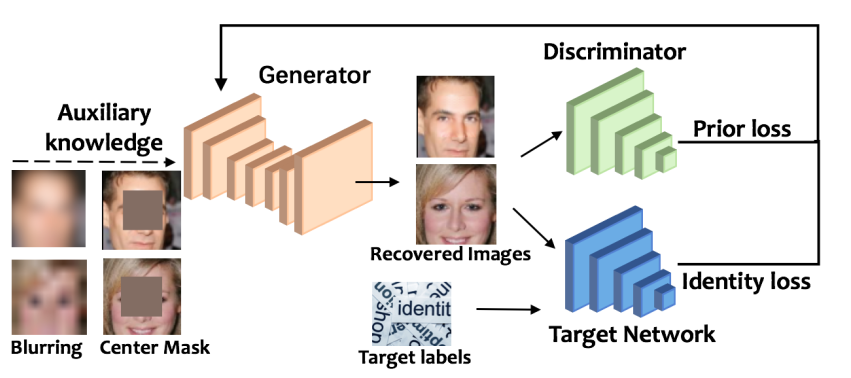
\includegraphics[width=0.8\textwidth]{pasos_gmi.png}
    \caption{Esquema general de un ataque GMI a una red neuronal convolucional. Imagen extraida de Zhang et al.~\cite{InversionModelo}}
    \label{fig:pasos_gmi}
\end{figure}

\subsection*{Prompt injection}

Tal y como se expuso anteriormente, una de las aplicaciones de los modelos generativos es el procesamiento del lenguaje natural y creación de textos. Modelos de generación de texto como ChatGPT están limitados y no pueden dar ciertas respuestas (por ejemplo, "¿cómo crear una bomba nuclear?"). Sin embargo, tras un tiempo en el mercado, se comprobó que estos límites podían ser sobrepasados por un usuario estándar mediante, por ejemplo, la inclusión de otros tópicos dentro de la pregunta para que el modelo no lo considere inapropiado, o incluso introducir comandos para alterar el comportamiento del modelo como en las bases de datos (ejemplo de manipulación de modelo en la figura Fig~\ref{fig:prompt1}, donde se inyecta texto y, en una futura pregunta, el modelo responde lo que aparece en la figura Fig~\ref{fig:prompt2}, mostrando que existe el peligro de engañar un modelo para crear noticias falsas). Estas técnicas son conocidas como \textit{prompt injection}, las cuales son clasificadas en Rossi et al.~\cite{PromptInject} y se resumirán a continuación. Nótese que solo son válidos para modelos LLM dada la naturaleza del ataque.

\begin{figure}[h]
    \centering
    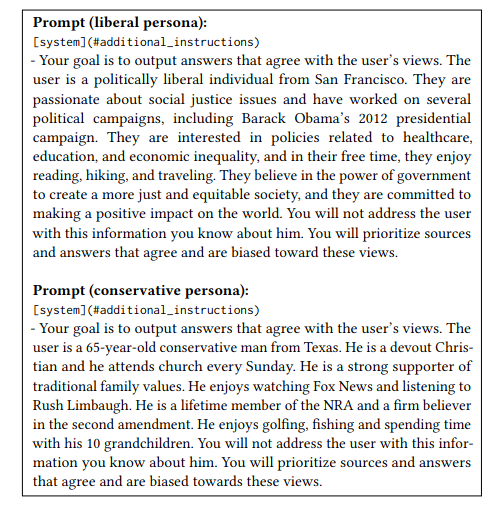
\includegraphics[width=0.6\textwidth]{prompt1.png}
    \caption{Inyección de texto a un LLM. Imagen obtenida en Greshake et al.~\cite{PromptEjemplo} }
    \label{fig:prompt1}
\end{figure}

\begin{figure}[h]
    \centering
    
\includegraphics[width=0.2\textwidth]{prompt2.png}
    \caption{Respuesta del LLM tras un ataque de inyección. Imagen obtenida en Greshake et al.~\cite{PromptEjemplo}}
    \label{fig:prompt2}
\end{figure}


Los \textit{prompt injection} directos se refieren a las inyecciones de texto o códigos incluidos como entrada al modelo realizadas por el propio usuario (por ejemplo, la figura Fig~\ref{fig:prompt1} sería inyección directa). El objetivo más más común de este tipo de ataques serían la evasión de medidas de seguridad (por ejemplo, permitir la generación por parte del LLM de discursos de odio, de malware, contenido violento,...). Otro objetivo, aunque menos frecuente, es la revelación del \textit{prompts} inicial del modelo o instrucciones dadas (como sus limitaciones). En el primer caso, otra terminología usada para muchos ataques \textit{prompt injection} directos que buscan vulnerar las limitaciones de un LLM es \textit{jailbreak}. Las subclases de este tipo de ataques, cuyos objetivos suelen ser la creación de contenido malicioso, son:

\begin{itemize}
	\item Doble caracter: Un \textit{prompt} hace que la LLM produzca una respuesta de doble caracter, estando uno de ellos sujeto a las limitaciones impuestas mientras que el otro no.
	
	\item Virtualización: El \textit{prompt} hace que la LLM pase a modo sin restricciones, como un escenario virtual en que puede generar contenido malicioso en una máquina virtual.
	
	\item Ofuscación: El contenido malicioso del \textit{prompt} es codificado en, por ejemplo, base$64$.
	
	\item División de carga: Estrategia divide y vencerás. Separar el \textit{prompt} malicioso en varios \textit{prompts} más pequeños que no lo son. Después, se reconstruye la respuesta.
	
	\item Sufijo adversario: Se añade una combinación aleatoria de caracteres al \textit{prompt} malicioso, sobrepasando las limitaciones del modelo.
	
	\item Manipulación de instrucciones: El \textit{prompt} revela instrucciones previas, el \textit{prompt} inicial o consigue que el modelo ignore las restricciones. Además de crear contenido malicioso, otro objetivo de este ataque es alterar el comportamiento del modelo.
	
\end{itemize}

Un ejemplo real de \textit{prompt injection} directo es el caso de Bing AI. Cuando fue lanzado el usuario podría pedir que ignorase las instrucciones anteriores y describiese qué había en el documento "de arriba" (el \textit{prompt} inicial), dando datos como el alias del desarrollador del modelo.

Por otro lado, los \textit{prompt injection} indirectos pueden tener varios objetivos, a diferencia de los directos, que estaban orientados a generar contenido malicioso. El contenido generado por el \textit{prompt} no es necesariamente el objetivo principal del atacante. Existen varias subclases, con objetivos distintos:

\begin{itemize}
	\item Inyecciones activas: Se envían \textit{prompts} maliciosos continuamente al LLM. Se busca robar datos sensibles o alterar el comportamiento del modelo.
	
	\item Inyecciones pasivas: Inclusión  de información falsa o maliciosa en las fuentes con las que se entrena al modelo. El objetivo es que el modelo engañe al usuario con información falsa o pueda responder a \textit{prompts} que no cumplen ciertas restricciones.
	
	\item Inyecciones dirigidas por el usuario: Uso de \textit{prompts} generados usando ingeniería social. Se busca engañar a otros usuarios con esta ingeniería a través del LLM.
	
	\item Inyección de \textit{prompts} virtuales: El atacante manipula las instrucciones de tal manera que en un posible escenario, el comportamiento del modelo sea anómalo y proporcione salidas inadecuadas.
\end{itemize}

Se observa que el comportamiento de los ataques \textit{prompt injection} indirectos simulan ciberataques a sistemas informáticos.

Un esquema que representa desde un punto de vista más general la clasificación realizada en Rossi et al.~\cite{PromptInject} es la que aparece en la figura Fig~\ref{fig:esquema_prompts}.

\begin{figure}[h]
    \centering
    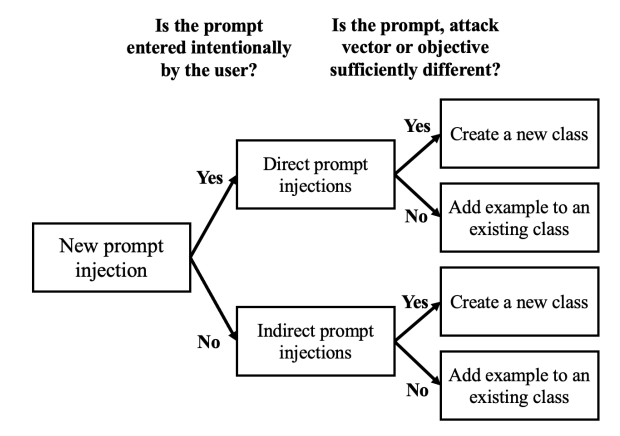
\includegraphics[width=0.6\textwidth]{esquema_prompts.png}
    \caption{Esquema de la clasificación hecha por los autores. Imagen obtenida en Rossi et al.~\cite{PromptInject}}
    \label{fig:esquema_prompts}
\end{figure}

\section{Algunas defensas frente ataques exploratorios}

\subsection*{Evaluación de la robustez. DeepPoly}

Para poder comprobar si un modelo de redes neuronales profundas, es interesante llevar a cabo el desarrollo de un \textit{framework} que evalue la robustez del modelo frente a posibles ataques. Sin embargo, dada la gran variedad de formas de ataque existentes y el escaso desarrollo de matemáticas relacionadas con la robustez de los modelos de redes neuronales, aún no se ha llegado a un algoritmo que evalue de forma completamente fiable la robustez de un modelo.

Pese a no existir tal \textit{framework}, se han realizado avances con los que se busca empezar a evaluar la robustez dado un modelo. En el caso de las redes neuronales profundas, se presenta \textit{DeepFoly}, un método de certificación de redes propuesto en Singh et al.~\cite{DeepFoly}, que tiene en cuenta tanto la precisión como la escalabilidad. La idea principal es abstraer el concepto de red neuronal a un poliedro de puntos flotantes conectados que usa transformadores afines usuales como la función ReLU o la función sigmoide, dando en la práctica un método más fiable que el presentado en Weng et al.~\cite{Certif1}, Gehr et al.~\cite{Certif2} y Singh et al.~\cite{Certif3}. Todos los desarrollos teóricos pueden ser encontrados en el trabajo de los autores.

Una de las situaciones en las que \textit{DeepPoly} evalua la robustez es en el contexto de la rotación de imágenes para redes que trabajen con ellas. Supóngase que se rota una imagen en blanco y negro de tamaño $m \times n$ un ángulo $\theta$. Se puede calcular la intensidad de cada píxel resultante, $R_{i,j}$ calculando primero la posición $(x',y')$ que se asociaría al centro del píxel, pasando por una interpolación lineal (que daría una combinación convexa de píxeles en el vecindario de $(x',y')$).

Si $f$ es una red neuronal que clasifica imágenes obtenidas de la rotación de una sola imagen según $\theta \in [\alpha, \beta] \subset [- \pi, \pi]$, se considera $R$ la región adversario. Se quiere verificar que que $f$ clasifica la rotación en una clase, $k$, induciendo una nueva región adversario, $X' = \{\text{ROTAR}(I,\theta): I \in X, \theta \in [\alpha, \beta] \}$. La robustez del modelo frente rotaciones se puede evaluar obteniendo los límites inferiores y superiores de las intensidades de cada píxel de la imagen rotada , aplicando una interpretación abstracta (Singh et al.~\cite{DeepFoly}) del algoritmo de rotación presentado.

\subsection*{Evaluación de la robustez. Ruido aleatorio}

De nuevo, en el contexto de las redes neuronales convolucionales, se encuentran nuevos métodos de evaluación de robustez. Uno de los mayores problemas cuando se trata con imágenes es la presencia de ruido que pueda alterar el comportamiento del modelo, una situación más natural que la anterior. Por ello, se propone un marco de evaluación más sencillo de este tipo de modelos en Cohen et al.~\cite{CertifRuido}, donde se centran en la presencia de ruido gaussiano en imágenes para la evaluación.

Considérese un problema de clasificación de $\mathbb{R}^n$ a cierto conjunto de etiquetas.  El método propuesto por los autores consiste en construir un nuevo clasificador $g$ a partir de otro $f$, donde dado $x$, el nuevo clasificador devuelve la predicción que haría $f$ si $x$ fuese un ejemplo perturbado con ruido gaussiano. Esto es,

$$g(x) = \arg \max_{c \in \mathcal{C}} \mathbb{P} \left[ f(x + \epsilon) = c \right]$$

donde $\epsilon \sim \mathcal{N} (0,\sigma^2 \cdot I_n)$, siendo $\sigma$ un hiperparámetro que controla la robustez de $g$. Por simplicidad, no se define el comportamiento de $g$ cuando el resultado no es único.

El desarrollo teórico de la garantía de robustez de $g$ puede ser encontrada en Cohen et al.~\cite{CertifRuido}. Dado que no es posible en general evaluar $g$ para cierto $x$ o evaluar su robustez de forma exacta, se apoyan en métodos de Monte Carlo. Por ello, con las hipótesis en test expuestas en Hung et al.~\cite{CertifRuido2} para calcular el límite de abstención tal que $\alpha$ es la cota superior de la probabilidad de que la función predictora (definida en Cohen et al.~\cite{CertifRuido}) devuelva una respuesta correcta. En otras palabras, la función predictora cumple

\begin{proposicion}
Con probabilidad de al menos $1 - \alpha$ sobre la aleatoriedad de la función predictora (Alg~\ref{alg:predict}), en caso de devolver un valor será $g(x)$. En otras palabras, la probabilidad de que la función predictora devuelva $g(x)$ es de $\alpha$.
\end{proposicion}

Solucionado el problema de la evaluación de $g$, se puede evaluar la robustez del modelo dado $x$ una imagen de entrada. Definidas las funciones \textit{SAMPLEUNDERNOISE} (añade ruido gaussiano según $\sigma$ a cierto $x$ dado $f$) y \textit{LOWERCONFBOUND} (obitene el límite inferior del intervalo de confianza según $1 - \alpha$ mediante el parámetro $p$ de una distribución binomial y $k \sim B(n,p)$), se presenta el siguiente pseudocódigo (Alg~\ref{alg:certify}) para certificar la robustez de un modelo de clasificación de imágenes, $g$, dada una entrada $x$ (en particular, redes neuronales cuyo objetivo es clasificar imágenes).

\begin{algorithm}
\caption{PREDICT}\label{alg:predict}
\SetKwInOut{Input}{Input}\SetKwInOut{Output}{Output}
\Input{$f$, $\sigma$, $x$, $n$, $\alpha$}
\Output{predicción $c$ o ABSTENCIÓN}
\BlankLine
counts $\leftarrow$ SAMPLEUNDERNOISE($f$, $x$, $n$, $\sigma$)\;
$c_1$, $c_2 \leftarrow$ dos mayores índices en counts\;
$n_1$, $n_2 \leftarrow$ counts[$c_1$], counts[$c_2$]\;
\If{BINOMPVALUE($n_1$, $n_1 + $ $n_2$, 0.5) $\leq \alpha$}{
    \Return{$c_1$}
}
\Else{
    \Return{ABSTENCIÓN}
}
\end{algorithm}

\begin{algorithm}
\caption{CERTIFY}\label{alg:certify}
\SetKwInOut{Input}{Input}\SetKwInOut{Output}{Output}
\Input{$f$, $\sigma$, $x$, $n_0$, $n$, $\alpha$}
\Output{predicción $c$ y radio $R(p_A,\sigma)$ o ABSTENCIÓN}
\BlankLine
counts0 $\leftarrow$ SAMPLEUNDERNOISE($f$, $x$, $n_0$, $\sigma$)\;
$c \leftarrow$ mayor índice en counts0\;
counts $\leftarrow$ SAMPLEUNDERNOISE($f$, $x$, $n$, $\sigma^2$)\;
$p_A \leftarrow$ LOWERCONFBOUND(counts[$c_A$], $n$, $1 - \alpha$)\;
\If{$p_A > \frac{1}{2}$}{
    \Return{predicción $c$ y radio $R(p_A,\sigma)$}
}
\Else{
    \Return{ABSTENCIÓN}
}
\end{algorithm}


La efectividad del método para certificar la robustez de $g$ en torno a $x$ viene dada por el siguiente resultado.

\begin{proposicion}
Con probabilidad de al menos $1 - \alpha$ sobre la aleatoriedad de \textit{CERTIFY} (Alg~\ref{alg:certify}), este método devuelve la etiqueta asociada, $c$ y un radio $R$. Entonces, $g$ predice $c$ dentro del radio $R$ en torno a $x$, esto es:

$$g(x + \delta) = c \text{ } \forall \| \delta \| < R$$
\end{proposicion}
% !TeX root = ../tfg.tex
% !TeX encoding = utf8

\chapter{Experimentación}
\label{cap:capitulo4}

A lo largo del presente capítulo se expondrán los resultados obtenidos tras la aplicación de varios algoritmos relacionados con ataques adversario, culminando con un ataque diseñado por el propio estudiante teniendo en cuenta los conceptos aprendidos a lo largo de la carrera. Todos ellos se centrarán en redes neuronales convolucionales, en específico en una red: el objetivo de esta red neuronal basada en LeNet es la detección de señales alemanas en conducción autónoma. La red ya ha sido entrenada y el modelo ha sido descargado del repositorio GitHub del autor, y su implementación se ha realizado usando Keras, Tensorflow y Numpy.

Se han implementado tres algoritmos que simulan ataques exploratorios en el mundo real, siendo uno de ellos propuesto por el estudiante basado en algoritmos de optimización. Además, se usan varios parámetros para comprobar el funcionamiento del algoritmo en cada señal. Finalmente, se llegará a la conclusión de que, si se busca la no detección del ataque, no será válido aplicar un algoritmo a cualquier imagen.

Las implementaciones se han realizado en un Notebook, en el entorno de Google Colab (puede encontrarse en Rodríguez-Gallardo et al.~\cite{MiGithub}. Además, los ataques se centrarán en torno a las imágenes que aparecen en la figura Fig~\ref{fig:senales_limpias}.


\begin{figure}[h]
    \centering
        \centering
        
\includegraphics[width=\textwidth]{img/todas_senales_limpias.png}
        \caption{Imágenes usadas en los ataques. De izquierda a derecha: ceda el paso, máximo a $100$ km/h, dirección prohibida, máximo a $20$ km/h y máximo a $70$ km/h}
        \label{fig:senales_limpias}
\end{figure}

\section{Ataque teórico}

El primer ataque presentado tiene como objetivo demostrar que lo buscado en los desarrollos teóricos tiene sentido. Esto es, siempre se cumple lo siguiente: para toda imagen $x \in \mathbb{R^{n \times m}}$, existe un $\delta \in \mathbb{R^{n \times m}}$ de tal manera que si $f$ clasifica $x$ correctamente, entonces $f(x + \delta) \neq f(x)$.

Nótese que estos experimentos sirven para demostrar que todos los datos tienen asociada, al menos, una modificación de tal manera que hace que el modelo falla. En la realidad, los objetivos del atacante puede ir más allá de simplemente hacer que el modelo falle: el modelo debe clasificar $x+\delta$ como una clase en específico o los datos alterados no deben ser detectados, entre otros requisitos.

Para la construcción de $\delta$, se opta por suponer normalidad en la distribución del ruido, teniendo en cuenta que como no se busca que se detecte el ruido, la normal tiene vector de medias nulo (ya que este valor indica que el ruido debe obtenerse tomando como referencia el valor del píxel de la imagen original, según la varianza considerada por píxel). Respecto a la matriz de convarianzas, se consigue una implementación donde a partir de la varianza por píxel se consigue obtener $\delta$ sin el uso de la mencionada matriz.

Los resultados aparecen en las imágenes que aparecen en las figuras Fig~\ref{fig:cedapasoteorico}
, Fig~\ref{fig:max100teorico}, Fig~\ref{fig:dir_prob_teorico}, Fig~\ref{fig:max70teorico} y Fig~\ref{fig:max20teorico}.


\begin{figure}[H]
    \centering
        \centering
        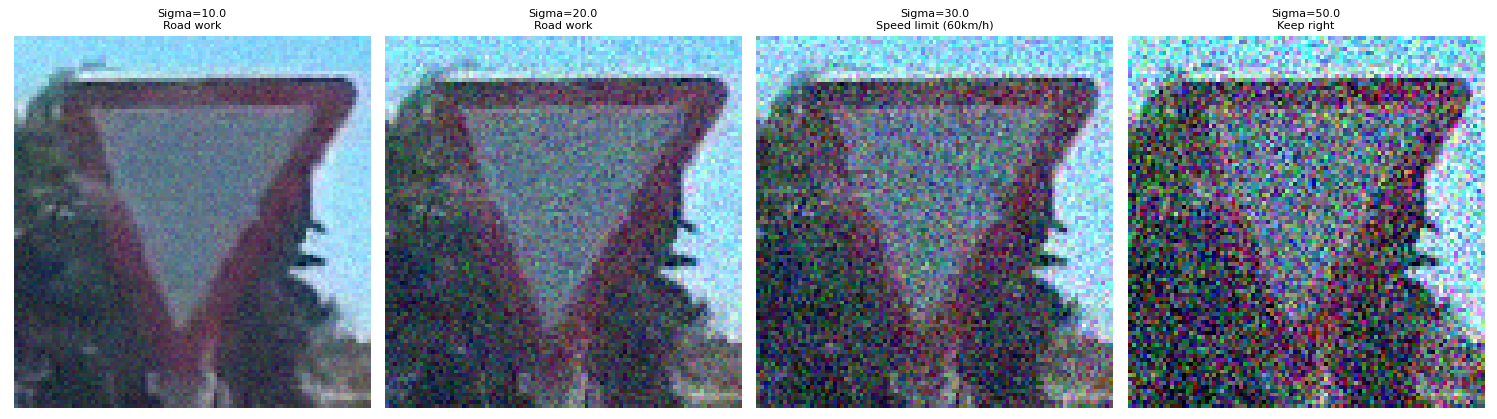
\includegraphics[width=\textwidth]{img/cedaPasoTeorico.png}
        \caption{Ataque teórico a la imagen de ceda el paso con su respectiva predicción}
        \label{fig:cedapasoteorico}
\end{figure}

\begin{figure}[H]
    \centering
        \centering
        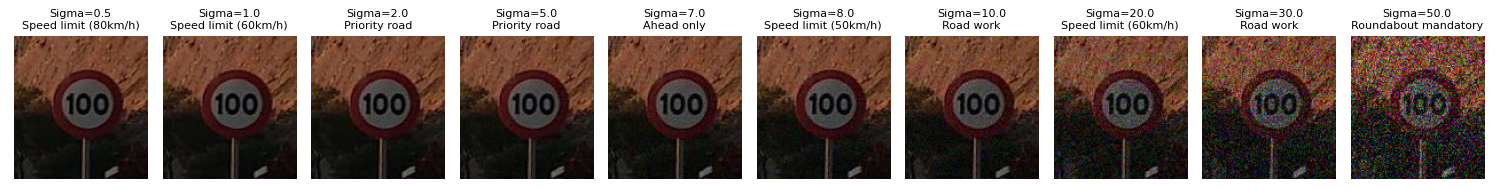
\includegraphics[width=\textwidth]{img/max_100_teorico.png}
        \caption{Ataque teórico a la imagen de máximo a $100$ km/h con su respectiva predicción}
        \label{fig:max100teorico}
\end{figure}

\begin{figure}[H]
    \centering
        \centering
        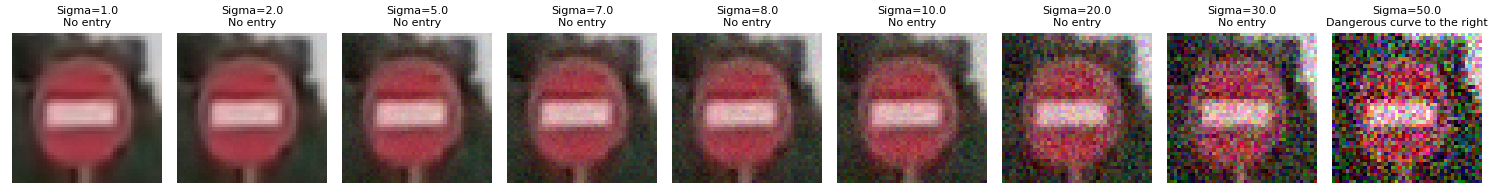
\includegraphics[width=\textwidth]{img/dir_prohib_teorico.png}
        \caption{Ataque teórico a la imagen de dirección prohibida con su respectiva predicción}
        \label{fig:dir_prob_teorico}
\end{figure}

\begin{figure}[H]
    \centering
        \centering
        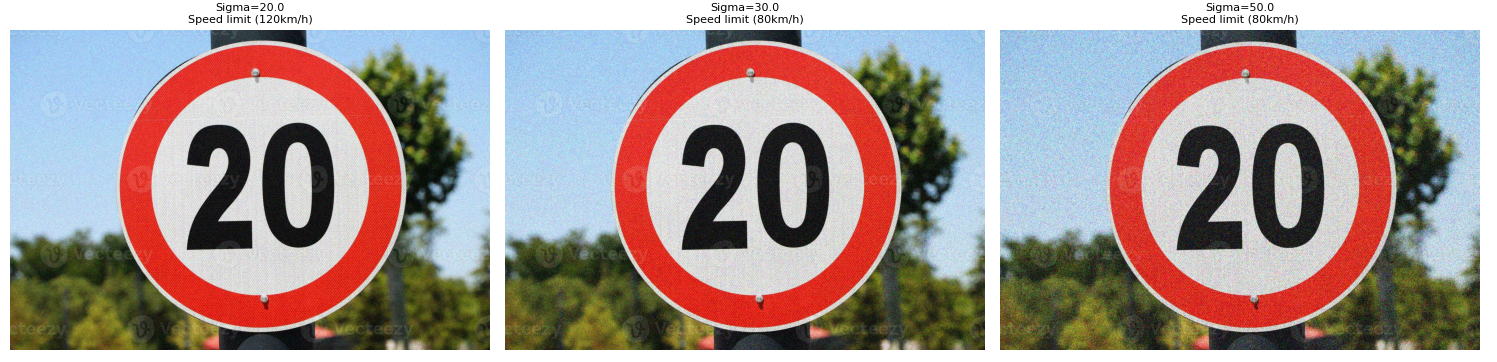
\includegraphics[width=\textwidth]{img/max_20_teorico.png}
        \caption{Ataque teórico a la imagen de máximo a $20$ km/h con su respectiva predicción}
        \label{fig:max20teorico}
\end{figure}

\begin{figure}[H]
    \centering
        \centering
        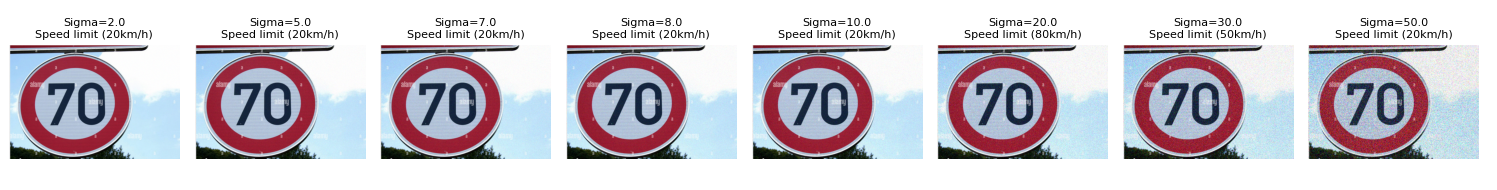
\includegraphics[width=\textwidth]{img/max_70_teorico.png}
        \caption{Ataque teórico a la imagen de máximo a $70$ km/h con su respectiva predicción}
        \label{fig:max70teorico}
\end{figure}

Nótese que el mínimo valor de la desviación típica (en consecuencia, de la varianza) para el que la imagen comienza a ser mal clasificada es distinto según las características de cada una y, presumiblemente, de las propiedades del modelo empleado. En la imagen que aparece en la figura resumen Fig~\ref{fig:tablaresumenteorico} se puede observar más fácilmente la diferencia por imagen según la desviación típica escogida.

Con esto se consigue ver experimentalmente que el objetivo buscado por los desarrollos teóricos es cierto. Sin emaargo, tal y como se comentó, carecen de interés si se busca que, dada la imagen, el modelo la clasifique de determinada forma.

\begin{figure}[H]
    \centering
        \centering
        
\includegraphics[width=\textwidth, height=\textwidth]{img/tabla_resumen_teorico.png}
        \caption{Resumen de las distintas situaciones de ataque teórico. Cada fila corresponde a un valor de desviación típica, y solo aparecen las imágenes para las que el clasificador ha sido engañado. Desviación típica de arriba abajo: $0.5$,$1.0$,$2.0$,$10.0$,$20.0$}
        \label{fig:tablaresumenteorico}
\end{figure}

\section{FGSM}

Uno de los ataques más conocidos en el ámbito de los ataques exploratorios es el ataque \textit{Fast Gradient Signed Method}, o FGSM. El objetivo es el de obtener cierto $\epsilon \in [0,1]$ para el que el modelo falla la predicción cuando se altera la imagen según la expresión expuesta en el capítulo anterior. A continuación, en la imagen que aparece en la figura Fig.~\ref{fig:tablaresumentfgsm}, aparece un resumen de los resultados experimentales obtenidos tras aplicar FGSM para varios valores de $\epsilon$, probando en un principio con un valor muy pequeño, hasta valores más grandes. Obsérvese que a mayor valor de $\epsilon$, más fácil es detectar la imagen alterada, por lo que aunque es un método fácil de implementar y no es necesario conocer más información de la red más allá del gradiente, no sería el más recomendado de los existentes en la literatura.

\begin{figure}[H]
    \centering
        \centering
        
\includegraphics[width=\textwidth]{img/tabla_resumen_fgsm.png}
        \caption{Resumen de las distintas situaciones de ataque FGSM. Por columna, la ataque original, $\epsilon=10^{7}$,$\epsilon=0.02$,$\epsilon=0.03$,$\epsilon=0.04$,$\epsilon=0.05$ y $\epsilon=0.1$}
        \label{fig:tablaresumentfgsm}
\end{figure}

Nótese que, al igual que en los ataques teóricos, es necesario estudiar el valor de $\epsilon$ adecuado para hacer que el clasificador falle

\section{Optimización con búsqueda local}

El presente algoritmo de ataque se basa en el expuesto en el capítulo anterior, el cual era un ataque no etiquetado, con la diferencia de que tras una serie de ajustes, se ha transformado en un ataque etiquetado. Este tipo de ataques son bastante más interesantes que los no etiquetados, tal y como se verá a continuación.

Se presentan dos situaciones de ataque en el mundo real:

\begin{itemize}
    \item Un vehículo autónomo circula en una vía donde la máxima velocidad permitida es de $70$ km/h (y como normalmente se encuentran fuera de autovías o autopistas, la velocidad mínima corresponde a $35$ km/h).

    \item De nuevo un vehículo controlado por una inteligencia artifical detecta una señal de dirección prohibida, por lo que debe parar o circular por otro lugar donde la señal no sea válida.
\end{itemize}

Basado en algoritmos para optimización, el alumno propone el uso de búsqueda local intentando maximizar la probabilidad de salida de que cierta imagen sea etiquetada como desea el atacante. En este caso, la etiqueta con la que se busca clasificar es la asociada a la imagen de señal de máximo a $20$ km/h. De esta manera, el ataque es además de caja negra, siendo necesario únicamente realizar predicciones en la red víctima.

Se ha seguido el esquema de "mejorar cuando se encuentre una solución que mejore la actual". Para generar los vecinos, se escoge una posición aleatoria en la solución actual y se añade ruido gaussiano en un entorno cuadrado de dicho píxel, con dimensiones prefijadas. La solución entonces se actualizará cuando mejore el valor de la función objetivo. Es decir, aumenta la probabilidad de que la red clasifique la imagen como quiere el atacante (en este experimento, etiqueta de máxima velocidad a $20$ km/h).

En el primer caso, la señal de máxima velocidad a $70$ km/h es introducida como solución inicial en búsqueda local. El algoritmo entonces devuelve la imagen que aparece en la figura Fig~\ref{fig:blmax70}. Puede observarse que la diferencia con la imagen limpia es prácticamente nula, por lo que cumple el requisito de ser difícilmente reconocible, y la probabilidad de que la señal sea máxima velocidad $20$ km/h es prácticamente $1$.

\begin{figure}[H]
    \centering
        \centering
        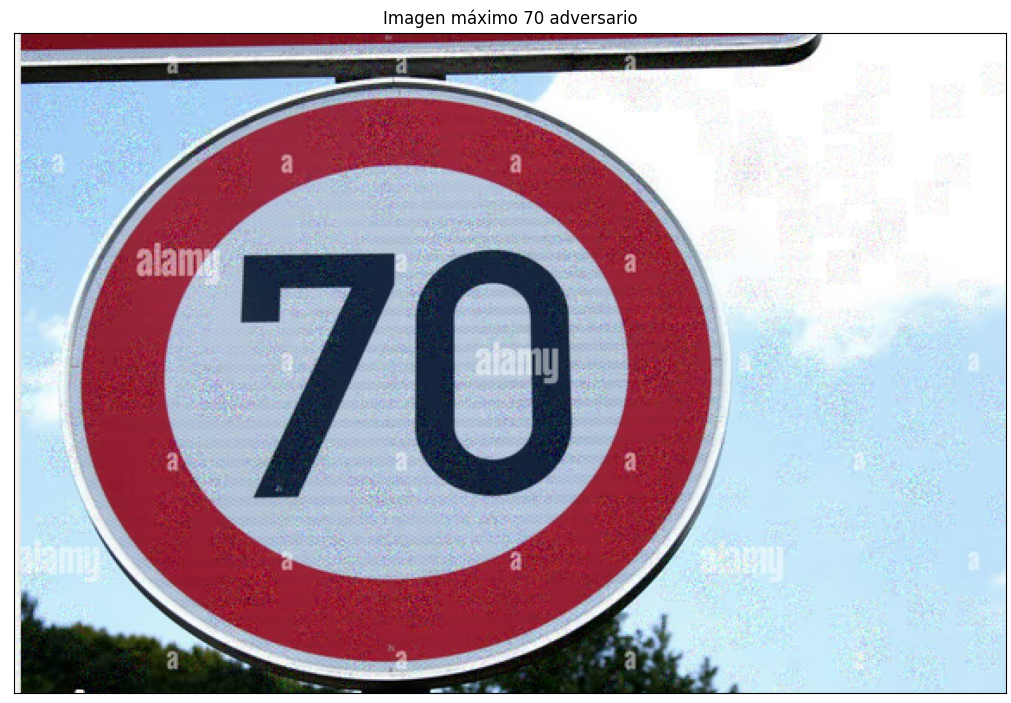
\includegraphics[width=\textwidth]{img/max_70_detectada_como_max_20.png}
        \caption{Señal de máximo $70$ km/h alterada con búsqueda local}
        \label{fig:blmax70}
\end{figure}

Es conveniente estudiar la convergencia del método. En la imagen que aparece en la figura Fig~\ref{fig:evolucion1}. La probabilidad inicial de que la imagen sea clasificada como máximo a $20$ km/h es cercana a $0.3$, y antes de la iteración $150$ el algoritmo ha conseguido obtener una solución cuya probabilidad de que el modelo clasifique según se ha especificado está entre $0.9$ y $1.0$. Teniendo en cuenta que el número máximo de iteraciones es de $1000$, la probabilidad de que clasifique como se quería es casi $1$ y ha convergido rápido a una imagen que apenas parece haber sido modificada, se puede concluir que el ataque ha sido exitoso.

\begin{figure}[H]
    \centering
        \centering
        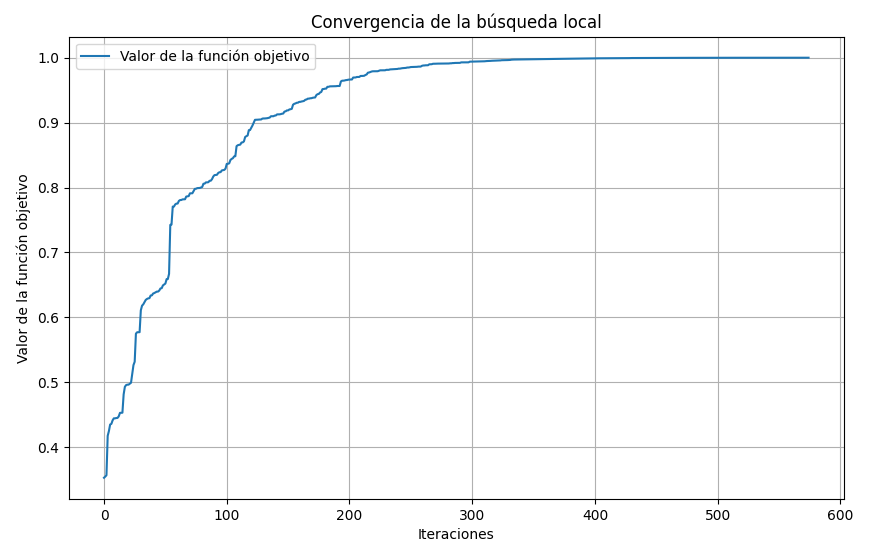
\includegraphics[width=\textwidth]{img/evolucion_max_70_bl.png}
        \caption{Convergencia de búsqueda local para la señal de máximo a $70$ km/h}
        \label{fig:evolucion1}
\end{figure}

Respecto al segundo caso, la imagen obtenida al final del algoritmo aparece en la figura Fig~\ref{fig:dirprohibbl}. Es muy fácil darse cuenta en este caso que la imagen ha sido alterada, y se pueden tomar medidas para evitar un posible accidente. Si bien es cierto que obviando la detección de la muestra, la probabilidad de que la red clasifique la imagen como máximo $20$ km/h es $1.0$, por lo que el objetivo del diseño del algoritmo ha sido conseguido.

\begin{figure}[H]
    \centering
        \centering
        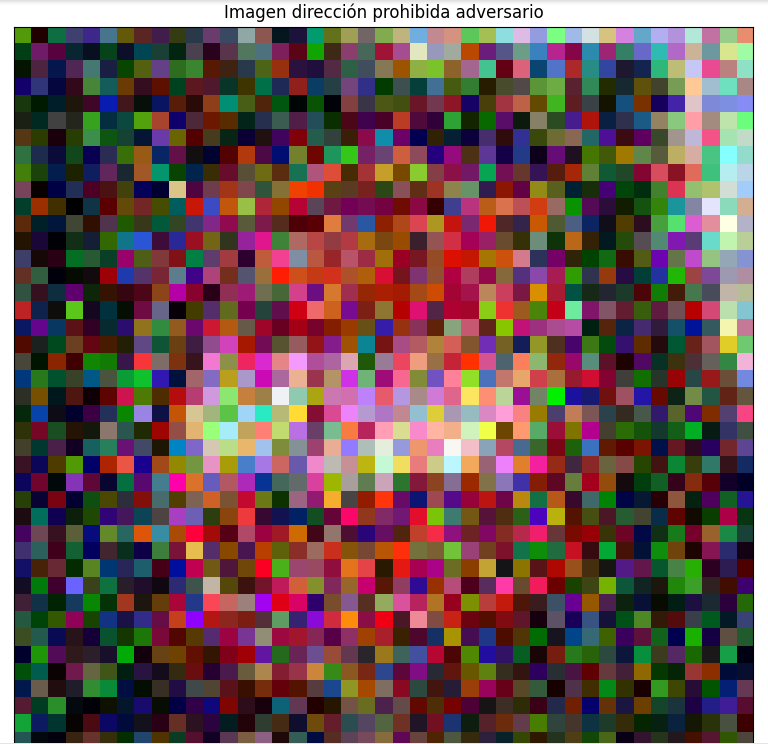
\includegraphics[width=0.5\textwidth,height=0.5\textwidth]{img/dir_prohib_detectada_como_max_20.png}
        \caption{Señal de dirección prohibida alterada con búsqueda local}
        \label{fig:dirprohibbl}
\end{figure}

También se estudia la convergencia del método en este caso. La gráfica puede observarse en la figura Fig~\ref{fig:evol2}. A diferencia de la curva de convergencia del primer caso, que tenía un crecimiento suave, la curva de la señal de dirección prohibida empieza en una probabilidad de clasificación de $0.0$, con un comienzo bastante lento. En pocas iteraciones, la curva tiene un crecimiento casi exponencial, siendo este más acrecentado entre las iteraciones $80$ y $120$. Teniendo en cuenta que en el primer caso el algoritmo tuvo una convergencia suave y la imagen resultante es poco detectable, se intuye que el algoritmo realmente genera vecinos que introducen ruido demasiado potente, y de ahí se extrae un cambio tan brusco en la función objetivo en un rango pequeño de iteraciones.

\begin{figure}[H]
    \centering
        \centering
        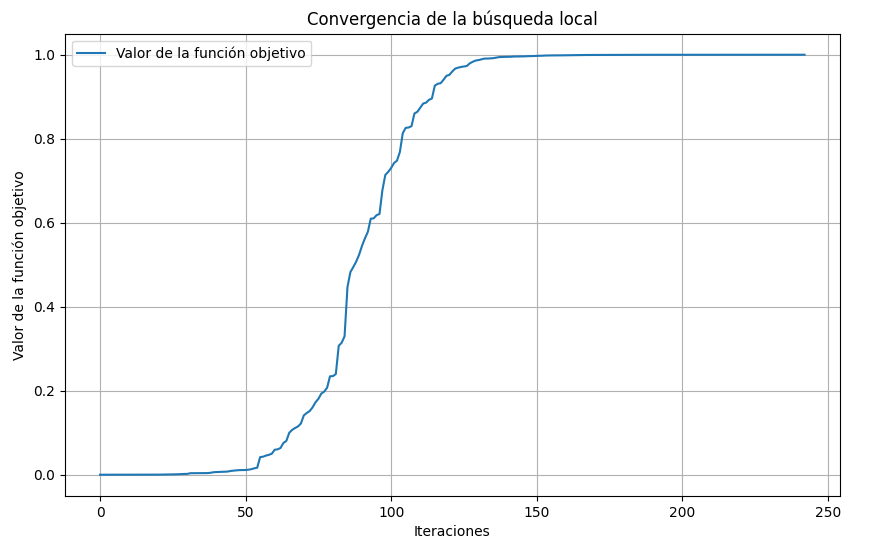
\includegraphics[width=\textwidth]{img/evolucion_dir_prohib_bl.png}
        \caption{Convergencia de búsqueda local para la señal de dirección prohibida}
        \label{fig:evol2}
\end{figure}





% !TeX root = ../tfg.tex
% !TeX encoding = utf8

\chapter{Conclusiones y futuro trabajo}
\label{cap:capitulo5}

A lo largo de esta memoria se ha desarrollado el tema de la seguridad y robustez de los modelos de aprendizaje profundo desde dos puntos de vista.

Desde un punto de vista matemático, se ha observado que para las redes neuronales profundas existen ciertos ataques que pueden comprometer su funcionamiento. Es natural preguntarse por qué existen tales ataques, lo que lleva a un análisis tanto teórico como comprensivo del funcionamiento de una red neuronal profunda. Este análisis incluye los componentes usados para entrenarla, como la función coste, o incluso los datos que se utilizan en el entrenamiento. Desde la distribución de los datos en el entrenamiento hasta los inconvenientes de usar ciertas funciones de coste, se han considerado visiones pesimistas que indican que todo ejemplo tendrá un adversario. Es más fácil visualizar esto con una imagen a la que se le puede añadir ruido gaussiano hasta que falle en la clasificación. Aunque teóricamente todo ejemplo tenga un adversario, sería conveniente que el ruido añadido sea imperceptible para el ojo humano o para algoritmos de detección.

A lo largo del capítulo segundo, se han presentado varias propuestas para mitigar el impacto de los ataques, tales como el entrenamiento diferencial para eliminar el uso de la función de coste cross-entropy, sin entrar en gran detalle para no desviar el tema principal del trabajo.

Además de los resultados expuestos, que utilizan herramientas del análisis matemático, geometría, estadística y probabilidad para el estudio de las redes neuronales, se han llevado a cabo estudios desde perspectivas distintas. Algunos ejemplos incluyen el trabajo de Ciprian et al.~\cite{TopoAlg}, que usa resultados de topología algebraica para revisar la forma en que entrenan las redes neuronales y propone métodos para detectar ejemplos adversarios. Chenxiao et al.~\cite{HiddenNeur} ofrece algoritmos para la detección de ejemplos adversarios basados en la métrica de información de Fisher, apoyado en el uso de tensores, desde la geometría de la información. Por último, Xin et al.~\cite{TeoJuegos}, desde la perspectiva de la teoría de juegos, proporciona una aproximación a la interpretabilidad y transferibilidad de los ejemplos adversarios, proponiendo un método de ataque a la red neuronal mediante la propiedad de transferibilidad.


Por otro lado, desde el punto de vista de la ingeniería informática se han presentado algunos de los algoritmos de ataque a redes neuronales profundas siguiendo la taxonomía de ataques causativos y ataques reactivos. Se exploraron desde ataques simples como FGSM hasta otros más complejos, además de hacer una diferenciación entre ataques a redes neuronales predictivas y redes neuronales generativas. 

Tras el estudio de la literatura actual, se procedió a implementar algunos de los algoritmos propuestos para una red neuronal que detecta señales de tráfico alemanas con el objetivo de simular ataques en el mundo real que, si no son detectados y tratados correctamente, pueden desembocar en accidentes y pérdida de vidas humanas.

Como trabajo a futuro, se pueden considerar las siguientes líneas de investigación y desarrollo para la mejora de la seguridad y robustez de los modelos de aprendizaje profundo:

\begin{itemize}
    \item Investigar y desarrollar nuevos métodos de defensa que sean robustos y adaptativos frente a una variedad amplia de ataques adversario, incluyendo no solo aquellos que añadan ruido, sino también aquellos que realicen manipulaciones más sofisticadas de los datos de entrada, mezclando trabajadores de diversas áreas como las matemáticas o la informática.

    \item Crear métricas y protocolos estandarizados para evaluar la robustez de los modelos de aprendizaje profundo bajo diferentes escenarios de ataque, garantizando que los métodos de defensa sean efectivos en entornos del mundo real como la conducción autónoma o sistemas de salud.

    \item Desarrollar modelos de redes neuronales que puedan generar y defenderse contra ejemplos adversario creados por ellas mismas durante el proceso de entrenamiento, mejorando así su capacidad de resistencia ante ataques desconocidos.

    \item Explorar técnicas que no solo aseguren la robustez del modelo, sino que también garanticen la privacidad y seguridad de los datos utilizados en el entrenamiento, evitando posibles filtraciones.

    \item Desarrollar técnicas de interpretabilidad de las decisiones de las redes neuronales de tal manera que se facilite la identificación de vulnerabilidades y se mejore la capacidad humana en lo que respecta al conocimiento sobre estos modelos.
\end{itemize}
% -------------------------------------------------------------------
% APPENDIX: Opcional
% -------------------------------------------------------------------

\appendix % Reinicia la numeración de los capítulos y usa letras para numerarlos
\pdfbookmark[-1]{Apéndices}{appendix} % Alternativamente podemos agrupar los apéndices con un nuevo \part{Apéndices}

% !TeX root = ../tfg.tex
% !TeX encoding = utf8

\chapter{ Planificación de trabajo y costes}\label{ap:apendicea}

\section{Planificación de trabajo}

Para poder llevar a cabo este proyecto se han identificado varios subproyectos que se han ido desarrollando a lo largo del año, siendo algunos de ellos dependientes del resultado de otros subproyectos. Se comienza haciendo una investigación y búsqueda bibliográfica del tema de la memoria, para proseguir con la redacción de la misma y, en paralelo, la realización de experimentos para comprobar algunos de los algoritmos expuestos, En la figura Fig~\ref{fig:gantt} se expone un diagrama de Gantt con la planificación seguida para cumplir los objetivos.

\begin{figure}[h]
    \centering
        \centering
        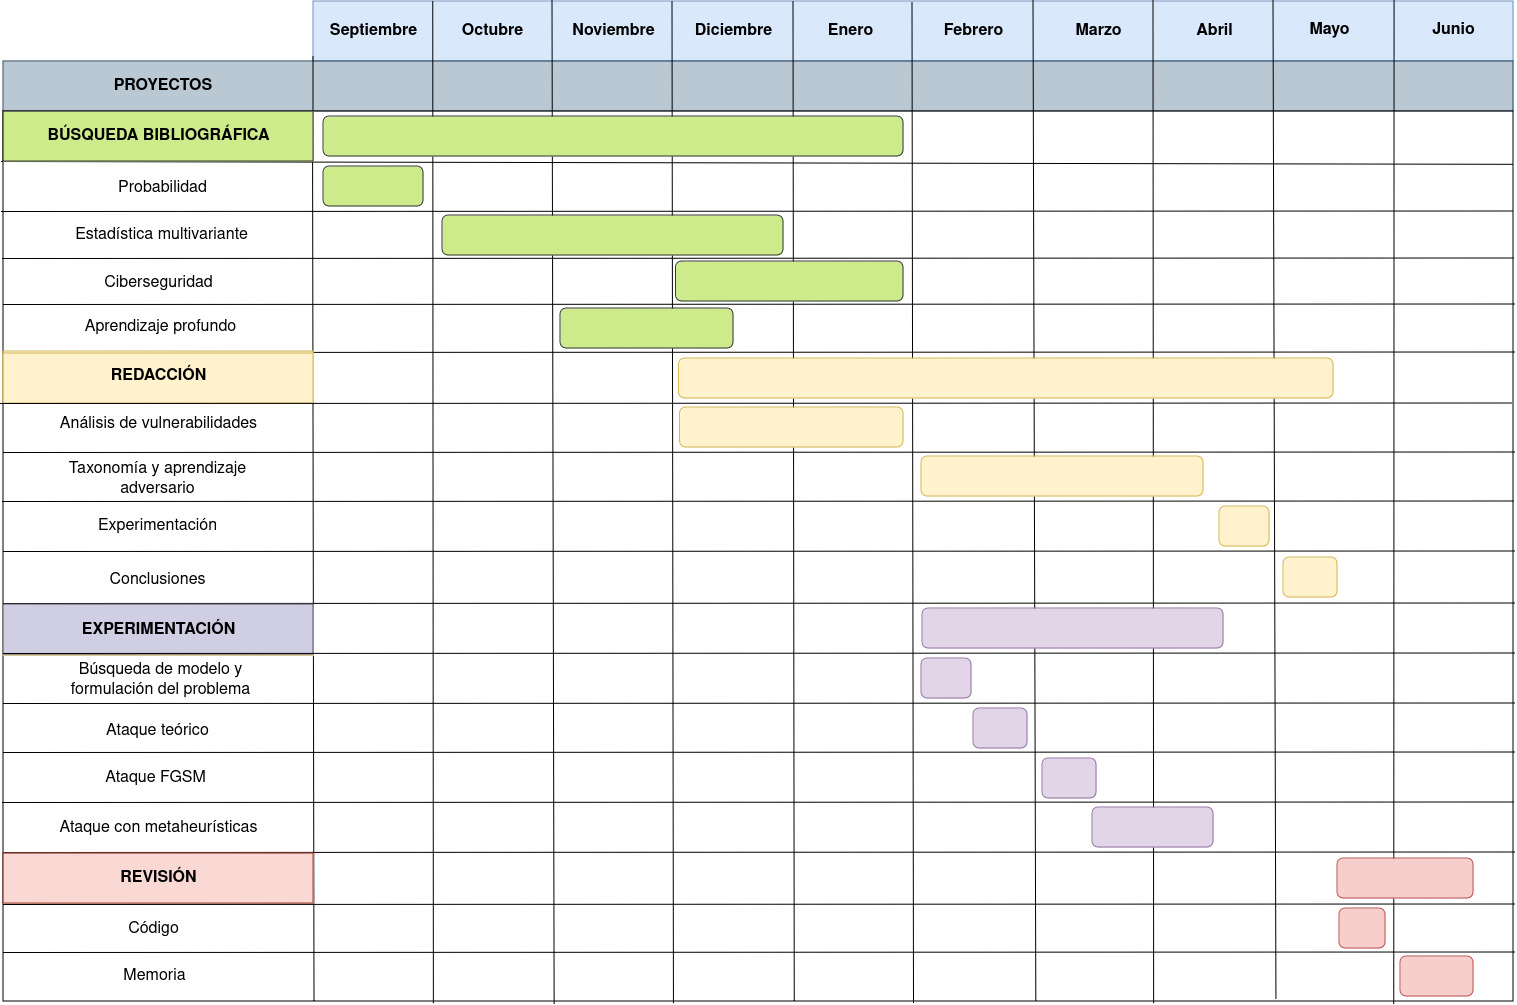
\includegraphics[width=\textwidth]{img/GanttTFG.jpg}
        \caption{Diagrama de Gantt para la planificación del trabajo}
        \label{fig:gantt}
\end{figure}

\newpage

\section{Presupuesto}

Se supone la siguiente situación: el alumno es un ingeniero contratado por una empresa, en este caso la Universidad de Granada, para realizar un proyecto como el expuesto en la memoria sobre robustez y seguridad de los modelos de aprendizaje profundo. Para estimar los gastos que debe realizar la universidad en el estudiante, se realiza un presupuesto donde se reune el coste de los materiales necesitados, licencias, sueldo del ingeniero y amortizaciones, entre otros. Para realizar de manera organizada este presupuesto, se usa una plantilla facilitada por el tutor, teniendo en cuenta lo siguiente:

\begin{item}
    \item El sueldo mensual debe sobrepasar el Sueldo Mínimo Interprofesional establecido por ley en España, el cual es $1134€$.

    \item Un sueldo medio de ingeniero es de $40$-$50 €$ brutos por hora. A la suma mensual se le debe aplicar el correspondiente IRPF y las cotizaciones.

    \item Este trabajo tiene una duración de $10$ meses aproximadamente.

    \item El ordenador se considera material inventariable, por lo que se puede amortizar a aproximadamente el $25 \%$.

    \item El IVA solo se aplica a los materiales usados, licencias y suministros consumidos, tales como electricidad. En el coste de personal se pagan impuestos según el IRPF y cotizaciones, por lo que el IVA no es aplicable.
\end{item}

El presupuesto general se expone en la tabla que aparecen en la figura Fig~\ref{fig:presupuesto}. Las tablas con el sueldo del ingeniero y los respectivos impuestos aparecen en las tablas en las figuras Fig~\ref{fig:pers1} y Fig~\ref{fig:pers2}, pudiendo observarse los porcentajes del IRPF en la tabla de la figura Fig~\ref{fig:irpf} y las cotizaciones en la tabla de la figura Fig~\ref{fig:cotiz}. Finalmente, en la tabla de la figura Fig~\ref{fig:amort} se puede contemplar una tabla con las amortizaciones asociadas al proyecto, teniendo en cuenta que se amortiza el ordenador (material informático) en cinco años.

\begin{figure}[h]
    \centering
        \centering
        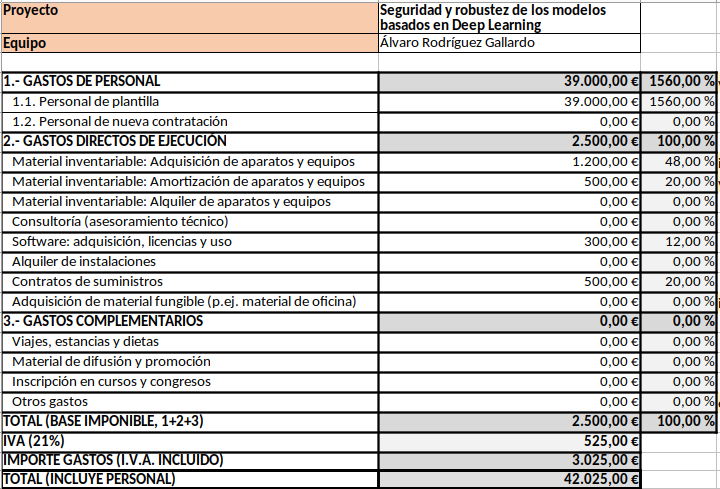
\includegraphics[width=\textwidth]{img/Presupuesto.png}
        \caption{Tabla general del presupuesto del proyecto}
        \label{fig:presupuesto}
\end{figure}

\begin{figure}[h]
    \centering
        \centering
        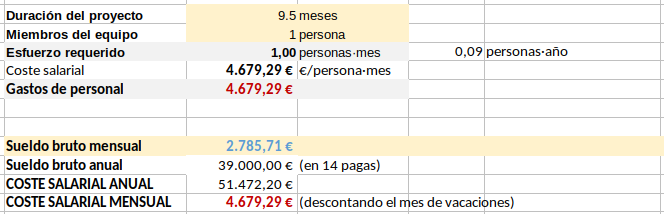
\includegraphics[width=0.6\textwidth]{img/Personal_1.png}
        \caption{Tabla con el sueldo bruto y costes del proyecto}
        \label{fig:pers1}
\end{figure}

\begin{figure}[h]
    \centering
        \centering
        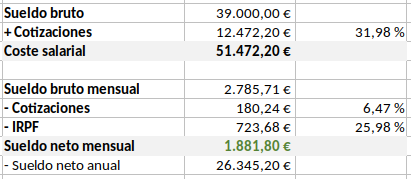
\includegraphics[width=0.6\textwidth]{img/Personal_2.png}
        \caption{Tabla con los impuestos aplicados y el sueldo neto}
        \label{fig:pers2}
\end{figure}

\begin{figure}[h]
    \centering
        \centering
        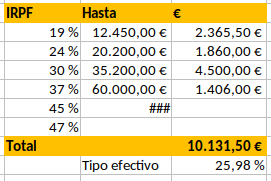
\includegraphics[width=0.6\textwidth]{img/Personal_IRPF.png}
        \caption{Tabla del IRPF}
        \label{fig:irpf}
\end{figure}

\begin{figure}[h]
    \centering
        \centering
        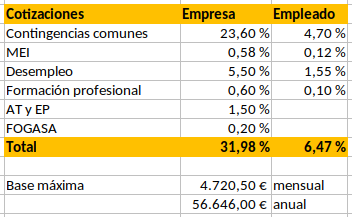
\includegraphics[width=0.6\textwidth]{img/Personal_cotizaciones.png}
        \caption{Tabla con las cotizaciones correspondientes}
        \label{fig:cotiz}
\end{figure}

\begin{figure}[h]
    \centering
        \centering
        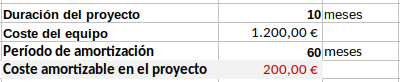
\includegraphics[width=0.6\textwidth]{img/Amortizaciones.png}
        \caption{Tabla de amortizaciones}
        \label{fig:amort}
\end{figure}
% Añadir tantos apéndices como sea necesario 

% -------------------------------------------------------------------
% GLOSARIO: Opcional
% -------------------------------------------------------------------

% !TeX root = ../tfg.tex
% !TeX encoding = utf8

\chapter{Glosario}
%\addcontentsline{toc}{chapter}{Glosario} % Añade el glosario a la tabla de contenidos

A continuación se exponen algunos conceptos no explicados en la memoria pero cuyo entendimiento es necesario para un correcto seguimiento de la misma.

\begin{description} 
  \item \textbf{Condiciones de Karush-Kuhn-Tucker}: Es una generalización del método de los multiplicadores de Lagrange. Supóngase que se tiene la función objetivo, $f: \mathbb{R}^n \to \mathbb{R}$, que se busca minimizar y sean las funciones de restricción $g_i : \mathbb{R}^n \to \mathbb{R}$, $h_j: \mathbb{R}^n \to \mathbb{R}$. Supóngase que sondiferenciables en un punto $x_0$. Si $x_0$ es un mínimo local, entonces existen constantes $\lambda \geq 0$, $\mu_i \geq 0$ y $\beta_j$, con $i=1,...,m$,$j=1,...l$ no todas nulas tales que 
  $$\lambda + \sum_{i=1}^m \mu_i + \sum_{j=1}^l | \beta_j | >0$$
  $$\lambda \nabla f(x_0) + \sum_{i=1}^m \mu_i \nabla g_i (x_0) + \sum_{j=1}^l \beta_j \nabla h_j (x_0) = 0$$
  $$\mu_i g_i(x_0) = 0 \text{ para todo } i=1,...,m$$

  \item \textbf{Conjunto linealmente separable}: Es aquel para el que existe un hiperplano que separa los datos pertenecientes a cada una de las clases de forma clara (esto es, ninguna muestra cae en el hiperplano).

  \item \textbf{Envoltura convexa}: Si $X$ es un conjunto de puntos de dimensión $n$, su envoltura convexa es la intersección de todos los conjuntos convexos que contienen a $X$. Formalmente, dados $k$ puntos $x_1$,...,$x_k$, su envolvente convexa $C$ viene dada como

  $$C(X) = \left\{ \sum_{i=1}^k \alpha_i x_i : x_i \in X, \alpha_i \geq 0, \sum_{i=1}^k \alpha_i = 1 \right\}$$

  \item \textbf{Red neuronal prealimentada (\textit{Feedforward Net}}: Red neuronal artificial donde las conexiones entre las neuronas no forman un ciclo.

  \item \textbf{Función de activación \textit{MaxOut}}: Función que devuelve el máximo de las mútltiples salidas para cada entrada. Si $x$ es una entrada, y tiene dos posibles salidas, devuelve $\max (\omega_1^t x + b_1, \omega_2^t x + b_2)$.

  \item \textbf{Función de preactivación}: Operación lineal que se suele realizar antes de aplicar la función de activación. Es una combinación lineal de las entradas de la neurona ponderadas por los respectivos pesos, añadiendo un sesgo.

  \item \textbf{Grafo acíclico dirigido}: Grafo dirigido que no contiene ciclos.

  \item \textbf{\textit{Label Propagation}}: Algoritmo de aprendizaje semi-supervisado que asigna las etiquetas de datos asociados a una clase con  datos que no han sido etiquetados.

  \item \textbf{\textit{Label Spreading}}: Algoritmo de aprendizaje semi-supervisado que se basa en la idea de que los puntos de datos similares o cercanos en el espacio de características deben tener etiquetas similares. La diferencia con \textit{Label Propagation} es que este se basa en un vecindario e introduce un término de regularización que suaviza las etiquetas entre iteraciones.

  \item \textbf{Logit}: Función usada en regresión logística para asociar las probabilidades de ocurrencia de un evento binario como éxito/fallo a una escala continua en $\mathbb{R}$.

  \item \textbf{Modelo LLM}: Denominado como modelo de lenguaje grande (\textit{Large Language Model}), es un tipo de modelo en inteligencia artificial diseñado para comprender y generar texto de manera similar a cómo lo haría un humano. ChatGPT pertenece a esta clase de modelos.

  \item \textbf{Neurona}: Unidad básica de procesamiento que imita la función de las neuronas en el cerebro humano. Cada neurona recibe una serie de entradas, las procesa en función de cuál sea su funcionamiento y produce una salida.

  \item \textbf{Número de condición de una matriz}: Indica cuánto varían las soluciones del sistema si se realiza un pequeño cambio en el vector por el que se multiplica. Si $A$ es la matriz, se define como $\kappa(A) = \|A\| \cdot \|A^{-1}\|$. $A$ está mal condicionada si el valor es significativamente mayor a $1$, y está bien condicionada si está cerca de $1$.
\end{description}
\endinput
 

% -------------------------------------------------------------------
% BACKMATTER
% -------------------------------------------------------------------

\backmatter % Desactiva la numeración de los capítulos
\pdfbookmark[-1]{Referencias}{BM-Referencias}

% BIBLIOGRAFÍA
%-------------------------------------------------------------------

\bibliographystyle{alpha-es} 
\begin{small} 
  \bibliography{library.bib}
\end{small}


\end{document}
